\setcounter{part}{-1}

\part[SCP-001提案]{
	SCP-001提案
	\protect\footnote{编者\QIS :\\ 
	SCP-001有多份提案,遂单独成一部分。\\ 
	又由于第一篇SCP-001其实是目录,所以内部文章编号从0开始。\\ 
	另外,由于大部分SCP-001提案旨在说明基金会的起源,推荐刚接触SCP系列的新人先跳过。在看过几十个SCP档案,对基金会设定有初步了解后再回来看001,可以获得更好的阅读体验。}
}

\setcounter{chapter}{-1}

\chapter[{SCP-001 等待解密[已锁]}]{
	SCP-001 Awaiting De-classification [Blocked] \\
	SCP-001 等待解密[已锁]
}

\label{chap:SCP-001.0}

\cl{

\GG{在管理者的命令下}

\GG{此文檔已被列為}

\bb{\Hg{\wred{最高機密}}}

}

\hr

\begin{scpboxbr}
\bb{通用說明 001-Alpha}:为防止SCP-001的真相泄漏,多份/零份伪造的掩盖文件与該份/多份真正的001文件一并储存。所有涉及到SCP-001本质的文件,包括一份/多份假文件,均由模因抹杀药物保护,如有未授权人员查看,将立刻导致心脏骤停死亡。除非是受到████-███-██████的指令,否則将SCP-001的内容透漏给公众者将会被处决。
\end{scpboxbr}

\hr

\cl{

\bb{\Hg{\wred{警告}}}

任何未经授权之人员访问该文档将立即被\bb{BERRYMAN-LANGFORD}模因抹杀觸媒处决。在未接种合適模因疫苗的情況下向下滚动页面将立刻导致心脏骤停死亡。

\bb{\GG{\wred{你已经被警告過了。}}}

}

\hr

\newpage

\begin{figure}[H]
	\centering
	
\includegraphics[width=\textwidth]{images/SCP.001.0.jpg}
\end{figure}

\cl{

\bb{模因抹杀觸媒启动}

\bb{检测到生命迹象}

\bb{解开安全锁}

\ii{欢迎,已获授权的人员,请选择您要看的文件。}

}

\hr

\begin{scpboxbrc}

代號:\hyperref[chap:SCP-001.sheaf.of.papers]{Jonathan Ball - 资料卷}

代號:\hyperref[chap:SCP-001.the.prototype]{Dr. Gears - 原型}

代號:\hyperref[chap:SCP-001.the.gate.guardian]{Dr. Clef - 守门者}

代號:\hyperref[chap:SCP-001.the.lock]{qntm - 锁}

代號:\hyperref[chap:SCP-001.the.factory]{Bright - 工厂}

代號:\hyperref[chap:SCP-001.the.spiral.path]{Dr. Mann - 螺旋路}

代號:\hyperref[chap:SCP-001.the.legacy]{Dr. Mackenzie - 遗物}

代號:\hyperref[chap:SCP-001.the.database]{S. Andrew Swann - 数据库}

代號:\hyperref[chap:SCP-001.the.foundation]{ Scantron - 基金会}

代號:\hyperref[chap:SCP-001.thirty.six]{Djoric/Dmatix - 三十六}

代號: \hyperref[chap:SCP-001.keter.duty]{Roget - Keter任务}

代號: \hyperref[chap:SCP-001.the.children]{djkaktus - 孩子们}

代號: \hyperref[chap:SCP-001.a.record]{Kate McTiriss - 一份记录}

代號: \hyperref[chap:SCP-001.the.broken.god]{TwistedGears/Kaktus - 破碎之神}

代號: \hyperref[chap:SCP-001.past.and.future]{Kalinin - 过去与未来}

代號: \hyperref[chap:SCP-001.the.consensus]{Wrong - 一致意见}

代號: \hyperref[chap:SCP-001.when.day.breaks]{S. D. Locke - 黎明将至}

\end{scpboxbrc}


\chapter[SCP-001 资料卷]{
	SCP-001 Jonathan Ball - Sheaf of Papers\\
	SCP-001 资料卷
}

\label{chap:SCP-001.sheaf.of.papers}

\bb{项目编号:}SCP-001

\bb{项目等级:}Keter

\bb{特殊收容措施:}到目前为止,没有足够并可行的收容程序去应对SCP-001可能造成的威胁。这部份是因为项目那有争议的本质和关于是否有必要收容争论。这些争论也充斥在项目那不断变化的等级和用于收容对象的程序上。尽管被认为有些偏执,目前的管理者们已将项目分类为Keter,甚至有人要求创造一个更高的级别并单独的应用在这个项目上,因为他们认为它是所有已知或可能存在的项目中最危险的。这个Keter的等级及对它有着不同态度的原因将在描述和补充说明中解释。

SCP-001现在存放在一个用密码锁上锁的由高强度聚合物制成的便携式保险箱里。存储的房间和箱子全天由安全摄像机监控。除非有全体O5长官给与的特别许可,箱子绝不能被打开。箱子本身保存在小而全部照亮的独栋站外建筑里,建筑竖立在███ ██████ ██████。 D级人员将被分派去守卫建筑,但在未经上述O5长官的同意时不得进入,否则将被立即处决。此站外建筑只用于存放SCP-001而且能在紧急情况下被线控引爆。

目前的管理者认为SCP-001代表着所有已知存在中对全国和全球安全的最大威胁。尽管过去在刚创建该项目的时候,SCP-001曾被保管在最低安全条件下,然而,由于某些特殊的环境会影响其能力的表现模式,进一步的研究项目是不被允许的。

\bb{描述:}SCP-001是一叠简单的文件,左上角被装订在一起。最上面的纸张是一个容易理解的封面,“关于特别对象的秘密报告——机密”。装订在后面的纸张的编号是不确定的,范围在三到三十内。该报告无署名并且来源不明。

本报告第一次出现是在███████ █, ████,当它出现在████████ █████的桌上时。本报告当时描述的是“The living room”(\hyperref[chap:SCP-002]{SCP-002})。满怀疑问的阅读报告后不久,有人通过电话联系████████ █████并告知其该项目的发现。接下来████████ █████再次阅读SCP-001,它不再描述“The living room”,转而描述“Biological Motherboard”(\hyperref[chap:SCP-003]{SCP-003})。████████ █████立刻关上了SCP-001,认为它应是一个不同寻常的报告,并开始寻找SCP-002原来的报告。毫无所获后,他又打开了SCP-001,这次它描述不是SCP-003而是“The 12 Rusty Keys and the Door”(\hyperref[chap:SCP-004]{SCP-004})。████████ █████再次关上报告并立即打开它,读到了“Skeleton Key”(\hyperref[chap:SCP-005]{SCP-005})。我们并不知晓████████ █████可能的下一步行动。而这一事件后不同长短的时间里,上述项目都被发现。

那些担忧SCP-001和所有其他已知的SCP有着相关性的研究都并没有充足的证据。然而,有一件事已经证实,即每一个与新的SCP被发现后都会在SCP-001的封面下面出现一个相关的报告。目前的管理者们把这一巧合作为存在因果关系的证明。

补充说明:不论是希望SCP-001要被分类进一个更高级的警告系统,或者是认为SCP-001本身是SCP们的造物主并需要特别收容,这两种意见都仍有待观察。然而,这种区别在目前管理者们的眼中是不重要的。因为事实仍然如此:除非SCP-001被打开和读取,没有新的SCP对象出现。正因如此,目前的管理者们拒绝重复过去的错误,那个已为SCP系列资料库带来了超过1000个SCP项目的错误。

那些有关于SCP-001本身是无害的,或其理论上可做为一个有益的预警系统,或者使用它作为先进的生物和非生物武器的货源的说法都没有动摇目前的管理者们。虽然也有争论,批评这些极端的抑制程序被应用到去关注一个没有显示邪恶特质和活力的项目等等。但管理者们提醒批评者们,这些程序的目的不是去收容项目本身,而是去防范其真正的威胁:与人类发生互动。

虽然,除非有上面提到的特别授权,目前的管理者们拒绝把项目从隔离中移出,但过去的管理者们也曾讨论过对其进行每日观察,并且未来的管理者们也毫无疑问会进行类似讨论。然而,目前的管理者们依旧认为,除非SCP-001被破坏,它应该被一直收容直到收容的责任落到了未来的管理者们身上。


\chapter[SCP-001 原型]{
	SCP-001 Dr. Gears - The Prototype \\
	SCP-001 原型
}

\label{chap:SCP-001.the.prototype}

\bb{项目指定编号:}\#86243AR-001

\bb{警告:}项目表现出侵略性并具高度危险性

\bb{项目描述:}

高六英尺五英寸,重97磅(平均值,±5-10磅),年龄未知,灰褐色皮肤(或许是挫伤),眼睛(?)颜色为牛奶蓝,没有头发。外表削瘦,骨骼和肌肉的结构不属于任何有记录的物种。腿部细长,末端为锐利的黑色尖刺。每只手有三只手指,末端同样有黑刺。腿部跟手臂均为躯干的两倍长。身上没有生殖器官、肛门、耳朵、鼻子或任何毛细孔。头成球形,相对于身体的比例来说很大,细瘦的脖子看似无法支撑。口腔延伸至头的一半,没有嘴唇,21颗牙齿随机排列在口中,许多都出现破损、腐坏或缺口。“眼”是一个大型牛奶蓝的球体,推测保存在头中或咽喉。似乎会在张开口腔时“滚”入其中。没有瞳孔或虹膜。

\bb{目前收容细节:}

房间墙壁嵌入铅,并保持以投光灯照明。温度保持在华氏98度(约摄氏36.6度)并且湿度保持在100%。房间由钢筋防爆门密封。外部区域由配备高供电照明灯的警卫巡逻。任何人员要进入房间需配备照明灯及焊接护目镜。尝试移动项目或未经授权进入房间的人员应立即射杀。

\bb{报告:}

本周初在瓜地马拉回收。第一目击报告是一群男孩在乡间道路上发现,他们称它“恶魔”。项目以生病或受伤的姿态出现。男孩们说它看起来颤抖着腿并气喘如牛。然后那生物抬高它的头并且露出它的“眼睛”。他们跑回家并回报当地的执法人员。数名当地人曾回报有维持数天的可怕咆哮及尖叫声。当地医院的记录显示有12个人遭受严重辐射污染,另有7人失踪。ADRX-19基地派遣了以Machoi将军为首的回收小组进行回收作业。在回收小组向监督者(Overseers)回报标准收容程序失败后,Hermann Keter博士创建了额外的收容程序。不幸的,在项目移动到ADRX-19之后,Keter博士在初次测试中死亡。

项目能够创造微小的奇点,作为传送与防御的手段。这些奇点会在几秒内消失,但大量辐射与重力仍然有能力对周边地区造成严重的损害。推测“眼睛”能够控制这些奇点,因为在创造奇点时总是会露出“眼睛”。杂食性,人类也是食物之一。项目在高温、高湿度及明亮或闪烁的灯光下会感到极度恐惧并且生病。项目无法穿过铅进行传送,而且在“生病”状态下无法创造奇点。在“良好”状态下,项目速度非常敏捷而且狡猾,已有数名回收小组成员在它的利爪及奇点下死亡。项目而偶会发出尖叫声,但与其所有沟通尝试皆宣告失败。

\bb{附录:}更多特殊个体的回报,使监督者考虑将ADRX-19转为专门的收容和收容设施。报告应在保密的考量下进行删改。


\chapter[SCP-001 守门者]{
	SCP-001 Dr. Clef - The Gate Guardian \\
	SCP-001 守门者
}

\label{chap:SCP-001.the.gate.guardian}

\begin{figure}[H]
    \centering
    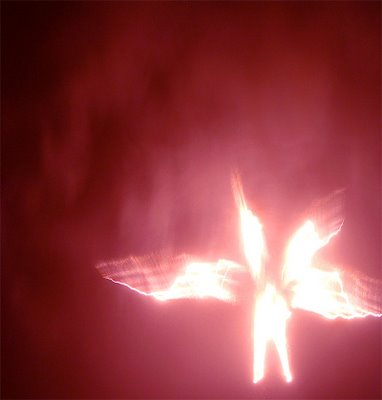
\includegraphics[width=0.5\linewidth]{images/SCP.001.the.gate.guardian.jpg}
    \caption*{在Site-0的有利位置拍摄的SCP-001图片。注意位于图片上方到两侧的四个燃烧的“翼”状附属物。}
\end{figure}

\bb{项目编号:}SCP-001

\bb{项目等级:}Euclid\slash Keter

\bb{特殊收容措施:}由于SCP-001的特性,没有任何监禁措施是必要的。对SCP-001的不间断监控必须在预定地点(Site 0)以外的安全距离(10公里以上)持续进行。Site 0的位置只有当前的SCP总管理员和一位被指派从Site 0监视SCP-001的信仰亚伯拉罕系信仰的监察者级探员(O5-14)所知晓。这位探员被授权当SCP-001开始活动时采取任何必要手段,并且需要当SCP-001的行为出现任何变化时立即警告总管理员和其他监察者级探员,因为这可能导致PATMOS XK级世界末日情境的开始。

如果SCP-001以任何形式开始活动,工作人员被要求立即考虑Patmos序列紧急指令。紧急指令Patmos的解法算式被保存在Site 0的被指派的监察者处,并且只在SCP-001开始活动的情况下才传输到SCP基金会的办公室。在紧急指令Patmos当中有着一项或多项重要角色的工作人员被建议做好以下准备工作:

\begin{itemize}
\item 和一种或多种有组织的亚伯拉罕体系的宗教保持良好关系。
\item 随身携带或手持以下物品:圣水,一件由一位主教以上等级的亚伯拉罕体系宗教教士所祝福过的玫瑰念珠,十架苦像,十字架,或其他象征物,一份亚伯拉罕体系宗教经本(托拉,圣经,古兰经),以及可随身携带的标准应急补给品(避难包)。
\item 在千禧年降临情境下,所有重要的人员都被指派一名非亚伯拉罕体系宗教信仰的副手,这名副手将会被告知原人员的紧急指令Patmos的备份的地址以及模因抹杀媒介的接种,并且准备好在必要情况下接替原职的任务。
\item 对所有其它涉及到可能的PATMOS XK等级世界末日情境的SCP保持熟知。
\end{itemize}

\bb{描述:}SCP-001是一个人形的个体,大约身高七百(700)腕尺,位于底格里斯河和幼发拉底河交口处附近的一个秘密地点,关于这个个体有下列已知特征:

\begin{itemize}
\item 从个体肩膀、背部、脚踝和腰部伸展出的数个发光的翼状形态附属物。尽管不能进行精确的计算,大部分的观察者给出的翅膀数目从二(2)到一百零八(108)个不等,平均数为4。
\item 一件武器,可能是一把剑或者刀(SCP-001-2)。通过光谱分析,这把武器从外观上看放射着温度足以匹敌太阳的火焰,尽管这极度的高温看起来并没有给周围的地区造成任何毁坏。任何接近SCP-001一公里以内的个体会立刻被这件武器攻击并彻底消灭掉。对SCP-001采取的任何形式的敌意行为都会导致攻击者的毁灭,不管距离多远。(参见事故报告:印度洋潜艇导弹实验,2004年12月26日)
\item SCP-001呈站姿,双手于身前握持SCP-001-2让其剑尖向下,低头呈祈祷状。自从建立者在{[}数据已编辑]年前所记载至今,SCP-001未曾改变过这一姿势。
\item 暴露在SCP-001面前的人类报告说在脑内听到了一个声音,向他们下达无法违抗的指令。最常见的指令是“忘记”,导致实验对象从SCP-001附近走开并且没有留下任何遇到过它的记忆。但是,在罕见的情况下,也会出现其它指令:最著名的指令就是下达给建立者的(“准备”)促使他成立{[}数据已编辑]来分类和保管所有对当前人类存在造成严重威胁的超自然以及异常物品。这就是现在被称为SCP基金会的组织。
\item 观察者报告说SCP-001是站在一扇巨大的门前面。长距离摄像偶然间探测到门内是一片田园树丛,里面还有无数的其他和SCP-001构成相类似的个体,还有几棵构成未知的果树。值得特别注意的是在树丛中间的地方有两棵巨大的果树:其中一棵,被注意到看上去是一棵普通的苹果树,但是另一棵树上的果实则完全不为地球上所知,被描述为{[}数据删除]。
\end{itemize}

建立者公开承认他相信SCP-001所守卫的门可能就是{[}删除],根据和古巴比伦文书和死海古卷的对比可知。在这个前提之下,我们可以推断被命名为SCP-001的个体可能就是{[}删除]

\hr

\uu{\bb{附录001-a:} 重新实验: SCP-001-2的有效杀伤范围}

\ii{1.实验A:一名D级人员被要求尽可能徒步接近SCP-001。}\\
结果:在和SCP-001发生视觉接触时,实验体被命令“离开”。实验体立刻转身离开SCP-001.尽管重复多次指示要求继续实验,D级员工拒绝遵守命令并被处决。在D级员工被处决时,所有涉及到实验的研究人员都被未知的力量消灭,推测是SCP-001-2。

\ii{2.实验B:一台遥控研究用机器人被控制从地面接近SCP-001。}\\
结果:在距离SCP-001一公里的时候,研究机器人被消灭了,推测是SCP-001-2的所为。所有后续的遥控侦查尝试都得到了同样的结果。

\ii{3.实验C:100个预先编程的研究用探针被命令从多个角度同时接近SCP-001}\\
结果:协调非常成功,100架探针同时通过了一公里标志线。然而,100架探针同时被SCP-001-2所消灭了。指派在Site 0的观察者报告说SCP-001-2看起来“同时向所有的方向发动了攻击”。SCP-001在此过程中姿势没有发生任何变化。

\ii{4.实验D:从3千米远处发射的线导导弹}\\
结果:SCP-001-2在武器穿过一千米距离时将其消灭,与此同时也消灭了发射场并杀死了所有人员。

\ii{5.实验E:从SCP核潜艇“鹦鹉螺号”上发射的多弹头洲际弹道导弹}\\
结果:参照印度洋潜艇导弹实验报告,2004年12月26日

\ii{6.实验F:\hyperref[chap:SCP-076]{SCP-076}和Omega 7特遣队被指示徒步接近SCP-001。}\\
结果:\hyperref[chap:SCP-076]{SCP-076}拒绝执行任务,尽管并没有得知任务的性质。在被问到为什么的时候,SCP-076回答说“不干,就是不干。”

\ii{7. 实验G:\hyperref[chap:SCP-073]{SCP-073}。由于实验F的结果,SCP-073在到达Site 0之前没有被告知他的目的地}\\
结果:SCP-073徒步接近地点。在看到SCP-001的时候,SCP-073变得非常悲伤并要求中断实验。SCP-073被命令继续实验。这时,SCP-073额头上的符号变成了{[}数据删除]。实验由于{[}数据删除]的缘故被终止。参见附录001-aa

\ii{附录001-aa:通过总管理员的命令,不再对SCP-001进行进一步的实验。不许再让任何SCP暴露在SCP-001前。SCP-001不可用于处理危险的SCP。细节部分请阅读修订版收容措施。}

\hr

\hr

\bb{附录:}在 ██-██-████,基金会工作人员接收到下面这条错误信息。

\begin{scpbox}

启动紧急指令 PATMOS-OMEGA

请注意:所有基金会工作人员

今天早上大约 ████:██:██ 的时候收到Site 0传来的下列信息。

\mono{SCP-001离开了它的位置。大门开启了。它们在前进。}\\
\mono{哦上帝啊,这真美……}

\mono{主的国来了主的国要来了主的国已经来了主将统治直到永永远远主的国来了}\\
\mono{主的国要来了主的国已经来了主将统治直到永永远远主的国来了主的国要来}\\
\mono{了主的国已经来了主将统治直到永永远远主他是上帝主他是上帝主他是上}\\
\mono{帝主他是上帝主他是上帝主他是上帝主他是上帝主他是上帝主他是上帝主}\\
\mono{他是上帝主他是上帝主他是上帝\bb{听吧以色列主我们的上帝主是唯一的}}

由于这一事件和最近\hyperref[chap:SCP-995]{SCP-995}的破裂,\hyperref[chap:SCP-616]{SCP-616}的开启和\hyperref[chap:SCP-098]{SCP-098}的启动的共同作用,基金会被要求立即开始准备应对XK级世界末日情境。\hyperref[chap:SCP-076]{SCP-076}和\hyperref[chap:SCP-073]{SCP-073}要立即被关押。所有人员解锁和编译紧急指令Patmos-Omega,并且遵从里面的命令。Site 19要被确保,并且一切非必要的SCP和人员都要被立即处决或销毁。重复,由于这一事件和最近\hyperref[chap:SCP-995]{SCP-995}的破裂,\hyperref[chap:SCP-616]{SCP-616}的开启和\hyperref[chap:SCP-098]{SCP-098}的启动的共同作用,基金会被要求立即开始准备应对XK级世界末日情境。\hyperref[chap:SCP-076]{SCP-076}和\hyperref[chap:SCP-073]{SCP-073}要立即被关押。所有人员解锁和编译紧急指令Patmos-Omega,并且遵从里面的命令。Site 19要被确保,并且一切非必要的SCP和人员都要被立即处决或销毁。重复,由于这一事件和最近\hyperref[chap:SCP-995]{SCP-995}的破裂,\hyperref[chap:SCP-616]{SCP-616}的开启和\hyperref[chap:SCP-098]{SCP-098}的起动的共同作用,基金会被邀球立即开始准被硬队XK级世界末日青境。\hyperref[chap:SCP-076]{SCP-076}和\hyperref[chap:SCP-073]{SCP-073}要立即被关押该隐和亚伯我的两个儿子,我来了所有人员解锁和编译看呐,我站在门前敲那门并且如果任何任任何ansdfysffollow aall alla khaf3242!\$\$@并且是是一个新的天堂一个新的地球和果实的\\
\textasciicircum \&@\#\$@\#@\#\$@\#\$███████\\
█████████\\
█████████\\
█████████\\
███{[}信号丢失]

\end{scpbox}

通过联系Site 0,O5-14回复说没有这样的消息从他那里发出并且SCP-001也依然静止。这条传输起初被认定为是恶作剧。然而,进一步的检验显示这条传输的时间标记在{[}数据已更改]年后的未来。因此可以推论{[}数据删除].

\hr


\chapter[SCP-001 锁]{
	SCP-001 qntm - The Lock \\ 
	SCP-001 锁
	\protect\footnote{
		编者\QIS :关于本篇的更多资料可查阅\autoref{chap:qntm.tips}和\autoref{chap:qntm.translator.append}。
	}
}

\label{chap:SCP-001.the.lock}

\bb{项目编号:}SCP-001

\bb{项目等级:}Safe

\bb{特殊收容措施:}SCP-001应当与所有相关数据一起锁在Site 10地下1层的重要档案保险库中。保险库是一个特别制作的的钢筋混凝土八棱柱房间(见附录U中的完整示意图),天花板上有一个 2000千克重,0.9米厚的时间锁。时间锁的时间表应该保密,只允许Y.Mirski博士查看。进入房间需要三重授权确认(例:出入卡+指纹+密码)。SCP-001是基金会最安全的所有物之一,因此这些措施主要是为了避免盗窃。

\bb{描述:}SCP-001是一个光滑、黑色而呈完美椭球形(大约15.1厘米×15.4厘米×16.5 厘米)的玛瑙宝石,上有斑驳的白色图案。它的外部,包括赤道和两极,包裹着繁复、分层而不规则的丝状黄金。在现在一般认为是“低处”或“南极“的地方,黄 金的被镂刻成宽阔的线条,但随着“纬度”的增加,花纹逐渐变得更加复杂精细。而接近“北极”,也称为“锁”或“奇点”(见下文的获取报告),花纹的复杂性 发展到超出了光学甚至电子显微镜的分辨能力。进一步的调查有赖于显微技术的进步。

宝石不断的发出少量(约34.5007至34.5010 毫瓦)的微波热辐射。金丝因此摸上去是温暖的,而白色斑纹发出的辐射比黑玛瑙部分要多。

除此之外,SCP-001是完全惰性的。它不会被任何形式的电磁辐射或超短波辐射穿透。而到目前为止,它是坚不可摧的(见下文:冥王星计划)。我们不过是从视觉观察后猜测它是玛瑙与金的组合物,因为取下样品做化学分析已被证明是不可能的。

\bb{冥王星计划主日志}

以下实验未能打开SCP-001:

\begin{itemize}
\item 传统的开锁
\item 蛮力攻击,如锤子,凿子,大锤,断线钳,焊枪,带锯等。
\item 在工业炉中持续加热到摄氏5000度(完全反射所有热能,并没有增加温度)
\item 直接使用工业切割激光(约160 kW\slash cm\textsuperscript{2},瞄准“锁”)(完全反射所有能量)
\item 老虎钳,汽车压碎机,钻石表面的液压压榨机(全部被毁)
\item 腐蚀性酸和其它强氧化物(无反应)
\item 高达0.5千吨当量的塑料与固体炸弹在近距离引爆(无效果)
\item 一个15千吨当量的原子弹头在近距离引爆[由Mirski博士授权](无效果)
\end{itemize}

\begin{scpbox}

\dd{冥王星计划将立即终止。——Hack博士}

\end{scpbox}

\begin{scpbox}

基金会正使用全部资源支持冥王星计划。——Mirski博士

\end{scpbox}

\bb{SCP-001的获取报告}

SCP-001的最早纪录在苏格兰贵族,第三代从男爵埃德温·杨爵士(Sir. Edwin Young)(1611-1677)的手写日记里。他按当时的习惯,拥有一个称为“珍奇密室”的小房间,收藏着一些神没有造出的人造物品,如雕塑、防腐处理过的生物和一些小玩意等等。Young在日记中提到了他在1654年穿越美索不达米亚沙漠时获得的“\ii{玛瑙与精细的黄金,是壹个被束缚的珍宝,优雅得超出了理智所能描绘}”。该日记显示,SCP-001被发现埋在一个“荒芜、被咒诅的地方,比远古更久远”的废墟中,Young认为那或许是献给“一个令人畏惧的死亡之神”的庙宇。废墟里有四个刻有符文的巨大石碑,石碑环绕着一个石头,SCP-001被包裹其中。Young的日记里有一张素描,上面画有 保存最完好的石碑最清晰那一面的符文,但他无法读懂符文,或是找到一个能把它翻译出来的学者。

Young前往废墟位置的那段旅程的纪录是不完整。因此废墟尚未被找到。

在Young死后,他那“\ii{奇特的天选之物}”静静的在仓库躺了数百年。1805年,他的后代将SCP-001捐赠给爱丁堡的苏格兰国家博物馆。博物 馆馆长把SCP-001视为一个古老,脆弱而无价的古代苏美尔金属工艺的遗产。因此它那异常的温暖、它的不可毁灭性和那不可能达到的微观结构都没有被他们 发现。不过,他们已经能够识别Young的素描上的符文,那是\ii{大约}公元前3400年的第三苏美尔楔形文字。目前只能翻译一部分:

\begin{scpbox}

通过损失和?????我们\slash 我?????[一个名词]\ii{apakht}[可能是一个专有名词]在这个结局\slash 定局??????????快乐+持久[可能是“保护”]

\end{scpbox}

进行翻译的McCandlish先生注解道:

\begin{scpbox}

这似乎是某种咒语,或许就是一个“收容咒语”。“apakht”就是禁锢在宝石里的那个东西的名字。

\end{scpbox}

最终,在1949年,SCP-001被半永久的展出。

2003年,一个正在度假的基金会工作人员注意到,SCP-001上白色斑驳图案类似于宇宙微波背景辐射。这种微波环绕着整个可见宇宙,03年初才被NASA的威尔金森微波各向异性探测器(Wilkinson Microwave Anisotropy Probe,WMAP)绘制出来。进一步的观察发现的两个图案是相同的。SCP-001(连同Young从男爵的日记)立即被基金会的一个外围组织买下, 并转移到Site-10由Q.Hack博士和Y.Mirski博士进行初步分析。

研究将继续由Mirski博士主持,Hack博士最近离开了基金会。

Young的日记还包括一些SCP-001的详细素描。其中一个素描,一件看上去像是钥匙的装饰华丽的小物体被安装进了“北极”里。但这件钥匙还没有被找到。


\chapter[SCP-001 工厂]{
	SCP-001 Dr. Bright - The Factory \\ 
	SCP-001 工厂
}

\label{chap:SCP-001.the.factory}

\bb{SCP-001是一名O5的故事}

晚上好,博士。

不,不,不用站起來。對,沒錯,我就是那個人。既然你我都明白,我們還是不要在這件事上耽擱太久了。你只知道我的號碼,而我對你的瞭解能讓我造一個你的複製品,連你媽都分不出來誰是真的。不對,這不是一個威脅,只是一個事實。

現在,關於我為甚麼來到這裡,你似乎碰巧發現了一些在你的權限之上的東西。恩,不對,碰巧發現不是一個正確的詞。發掘?或許更準確。而你正在接近一個危險的臨界點,到那時任何進一步的發掘都會以一個致命的槍傷作為句號。這對於我們的事業將會是個可悲的情形,因為除此之外,你依然是一個非常棒的研究員。因此,你將會得到只有極少數基金會中人曾得到過的東西:一個解釋。

沒錯,當你第一次探索SCP-001時,我們就已經警惕了。每一個曾短暫接近它的研究員都會忍不住往裡面看看。大多數都滿足於他們發現了帶著火焰劍的天使,它已經埋在足夠深的等級下了。但接著你開始調查The Factory,我們就知道你不會停下。所以,我將告訴你那個清晰而簡單的答案。

The Factory就是SCP-001。

但這個真相是永遠不會被寫下來的。這是我早在基金會創立初期就決定的,而且我仍然堅持這個決定。你們這些研究員實在太有好奇心了。我不知道哪件事更令我恐懼:我們永遠不會瞭解The Factory,還是我們有一天會瞭解它。好吧,我知道你渴望知道更多。

The Factory是在1835年建立的。那時它叫做The Anderson Factory,因一位非常富有企業家,其創始人詹姆士・安德森(James Anderson)而得名。它是,呃,我只能告訴你它是在美國成立的,並且是到那時為止最大的工廠,最寬處有一英里(1.6公里),所有建築都有3層樓,大門前還有一個專供Anderson使用的7層高塔。它被設計為工廠的最終形態,能夠處理所有的東西,包括員工的住房。人們可以在這裡出生、工作、生活、死亡而不需要離開工廠的範圍。人們的工作範圍極廣:從牛的養殖到屠宰,紡織,以及世界上一切工作。

但是,沒人知道James Anderson是一個撒旦的崇拜者。他有很大可能信奉一些異教的神靈。他對於工廠裡建築的位置和機器的擺放有非常嚴格的要求。工廠的幸存者聲稱建築的地板上刻滿了只有當鮮血流過時才能看到的神秘符號⋯⋯當然,幸存者還告訴了我們一些其他的東西。他的錢是從工人階級的血汗,甚至工人階級的屍體上賺來的。他在日記裡認為工人不過是一種比人類低賤的東西,放在地球上就是來為他服務的。

當然了,在那個時候還沒有人瞭解他的邪惡嗜好,因而他的工廠吸引人們蜂擁而至。有一個地方能同時解決工作和生活?好吧,人們理所應當的想要進去!至於嚴苛的工作時間、惡劣的工作環境,殘酷成性的保安,和其他所有的一切古怪,都沒有關係。工廠的工人們被迫一天工作16個小時,從日出幹到日落,星期天才能停工。工人甚至沒有獨立的房間,要與另外8人分享房間,三班倒的輪流去睡覺,保證工廠全天有人幹活。從沒有人聽說過醫療。如果你因為你的職責受傷了,你只會被要求繼續幹下去,那些傷得太重而無法工作的人會被保安拉走,沒人再聽說過他們。

整整40年,安德森工廠大量製造了所有人類所需的產品。肉、衣服、武器。不會有人介意牛肉裡面可能混合著人肉。別去想武器是在鮮血裡淬火的。不用去管衣服的顏色是來自⋯⋯呃,你懂的。確實有泄漏出去的謠言,但是那些產品那麼好,幹嘛抱怨呢?直到有人逃了出來。

我從沒有見過那位勇敢追求自由的靈魂,不過她想盡辦法見到了格蘭特總統。在1875,格蘭特總統尋求我的幫助。當時我是⋯好吧,這不重要。我只會告訴你我是一名軍人,某種軍人,而且我的夥伴們也是。我們有150位好兄弟和几位姐妹,接一些常識不會接受的工作。我們清洗過一些南部聯盟的頑固份子,以及我們在南方找到的更壞的東西。於是,我們做了一些調查,並不喜歡我們看到的東西。我們闖進了工廠,承擔這項重擔。

我並不完全記得那個工廠陷落的夜晚了。許多記憶在我的腦子裡攪成一鍋粥。一些片段常會閃現出來,有時是許多人被一根鎖鏈拴在一起,活在死亡的邊緣,你極難分出來哪塊肉是誰的。孩子們活在機器的支配下,身上大部份的肉都已經被轉輪、齒輪之類的機器從骨頭上剔掉了。

沒事,我沒事。我已經很久沒有回憶這些東西了。工廠的保安並不是問題,但Anderson的作品很快出現在我們面前。他把很多受傷的工人拉走,然後,嗯,在他們身上做試驗。人類,如果你還能把他們稱為人的話。許多種類的手臂縫在他們身上,有些還裝上了動物的身體,是超出人類最荒誕邪惡的噩夢的恐怖怪物。他們不斷湧來,不能稱之為活著的生物一波波的出現。那個晚上我失去了許多戰友。後來我們發現了Anderson的培育地下室,一個只有8歲的小女孩被綁在牆上,被變成了-

對不起。即使在超過一百年後的今天,這些記憶仍仿佛滿是血色。我們找到了蜷縮在他的辦公室裡的Anderson,用他的腸子把他吊死在高塔的窗外。在他死亡的過程中,他不斷狂笑,大叫說這不是問題,我們可以殺了他,但他的工廠,The Factory,不會停工。24小時後他仍狂笑不止,我們最終放他下來,掏出他的內臟,每件都切成四塊,再把剩下的部分燒成灰燼。整個過程他一直在狂噴褻瀆之詞,我不想回憶那些話。

我們用了一個星期去清理這片區域、釋放工人、紀錄每一件我們在地下室和昏暗的房間中找到的東西。我們拿出那些看上去有用的東西,存放在大門旁的一座房子裡。嘗試去弄懂每一件東西。我們有150位夥伴在那個晚上進到地獄裡,只有93人出來。而一星期後只剩下71人了。

而那些我們在裡头找到的東西,我的天哪。好吧,你已經在基金會工作過一段時間了,他們應該不會讓你太過驚訝。不過當時我們可是第一次看見會發射真子彈的玩具槍;能把碰到它的皮膚剝下來的搖搖;只對人體起作用的大錘;一種跑得比當時所有東西都快的骨駭馬;如同暗夜親自編織的斗篷,能讓穿上它的人來到一個虛無的維度,那裡有⋯⋯我又失態了。我們找到了很多器具,既不可思議,也很可怖。接著我們面臨著一個抉擇。

我把隊伍裡最高級的幾個人召集來,恩,我想想,我們最好稱他們為長官。我們設法去弄清楚我們接下來該幹甚麼。每個人都有不同的想法。Chaplain變得有點瘋瘋癲癲的,覺得這些對象都是神賜予我們的奇蹟,要像對待聖物一樣崇拜它們。Marshall還有他的跟屁蟲Dawkin認為這些是工廠造出的好寶貝,要繼續製造它們然後賣給出價最高的人。Injun,我們都叫他Bass,因為他的聲音像男低音一樣,說這是令人厭惡的東西,聲稱無論如何他都會搜尋並銷毀所有他找到的東西。Smith想到我們應該先釋放所有勞工然後把他們帶回總統那裏。我們在那裏爭吵了幾小時,幾天,想辦法解決這些。至於我,我覺得我們正坐在一座金礦上面,行了別那樣看著我。雖然很危險,但我們可以利用這些東西,這些對象,去搜捕那些我們曾在南方偶然遇到的駭人之物,以及其他需要全世界共同應對的怪物。讓這個工廠用在正道上,一個可以收容這些東西的地方,想辦法讓它們為人類同胞服務,至少保護人類免受其害。

我想你應該已經猜到接下來發生甚麼了。Chaplain在一天晚上帶著他的崇拜者偷偷離開了,還拿走了幾件小物品。我們把Marshall攆走因為我們發現他在⋯⋯濫用職權。他保證他一定會報復我們。卑賤的Dawkin該死的帶領他們那群人和一些重要物品離開了。Bass和他的人努力的去點燃工廠想把這些該死的東西燒掉卻徒勞無功,後來他們也走了。Smith也跑去向總統匯報。我最終讓他保證會告訴格蘭特工廠已經徹底毀掉了。我有一個大計劃。

當然了,想要實現一個大計劃是有點困難,特別是只有12個人和你一起工作的時候。不過我們還是開始了。

計劃運行得很順利,暫時的。我們已經有了這些神奇的玩具,想要招人跟我們一起工作就變得很容易了。在那個時候,離開電就像走出村子一樣簡單。我們知道我們需要甚麼,也知道我們會變成甚麼。

Leventhal開始得到我們的支持。他搞了個小發明,弄到了一大筆投資,都很有用。White和Jones則開始得到我們⋯⋯其他人的支持。在我們搞定工廠之前的工作中我們已經發現了一些與某些人有關的有趣的東西。那些當權者不會想要泄漏出去的秘密。而且,因為我們新的根據地讓我們能更好的守住這些秘密,越來越多的人跑來想讓我們處理他們的秘密。勒索是個骯臟的詞,不過很管用。Bright,Argent和Lumineux著手紀錄項目。Light和Bright的老婆,她們是護士,確保我們保持健康。嘿。算了,只要記住Light就可以了。在那個時代,她在衛生方面有著許多獨特的見解。Czov,Fleischer和Carnoff處理軍隊訓練的事。Tesla和Tamlin負責找出利用項目的方法,在不會暴露我們的情況下。

我們的效率高得驚人。一個城市圍繞著The Factory建立起來了,我們開始叫它作Alpha站點,而且它還是自給自足的。特工、研究員、各種熟練技工⋯⋯當然,我們不依靠那些當權者,而是靠這些工作人員。我們不斷發展壯大。

…

不好意思,我已經是一個老頭了。我知道我不願意正視它,不過我的身體在撒謊。我的腦袋⋯⋯並不總是記得准確。有時我會沈浸在回憶裡。事情變得令人困惑。不過在很長一段時間裡,一個顯而易見的事實是:我們在利用the Factory。總是能在裡面找到更多的空房間去儲存東西。那個時候我們還用“東西”來稱呼它們。不需要跳過這段,不需要。我們認為我們已經馴服了the Factory。這是我不停止這項工作的原因之一。但如果現在有甚麼事情是我確信的,那仍然是人類永遠不能馴服這些東西。收容它們就好了,就像那位你我都曾見過的Able一樣,馴服它們?不可能。

大約十年之後,我們已經組織的很好了。13位創始人只用編號作為代稱,不再用名字。大家都知道怎麼樣讓事情運轉良好。並且,如果有一兩件東西在the Factory裡消失了,依然如此?而且有時是D級人員消失?甚麼?沒錯,我們那時就已經有D級人員。用過就丟(Disposables)。這就是字母D的由來。肯定要有一些人給我們試驗那些東西,Tesla和Tamlin對此非常堅決。但是,沒錯,有時我們會失去一些無關緊要的人。Adam⋯⋯抱歉,是Dr. Bright喜歡說這是the Factory在讓我們“留下買路財”。你不可能甚麼都不付出就有收獲。

到了1911,一切都失敗了。那些傢伙⋯⋯我們稱之為小仙子。那些傢伙全族都棲息在我們旁邊。它們看上去跟你我長得一模一樣。唯一明顯的區別在于對鐵過敏。對,這就是為甚麼我們叫它們作小仙子。不過,你從沒聽說過它們是很正常的。為甚麼?因為那個時候基金會就已經把它們全族都滅絕了。連根帶葉的。並且我也動手了。

我們已經被它們當成獵物一段時間了。我們之前也碰到過它們幾次,都把它們成功搞定了。所以,當某位王室成員來向我們尋求幫助時,我們當然會想要讓他們欠我們人情。人人都喜歡讓別人欠自己人情的。我們派了一對人員去幫忙,稍微關注了一下,覺得這不過是一次狩獵派對。下次我們看見隊員們和那個王室成員,他們的頭都被插在杆子頂,系在小仙子騎的生物的馬鞍上,它們來攻擊the Factory了。

很可怕。

三個字,信息量太大了。我從來沒有⋯⋯抱歉,請給我一點時間。我從來沒有告訴任何人這個部分。你應該覺得你很幸運。而且,如果你把我將要告知你的事情的任何一點點說給其他人,我不僅僅會殺了你,還會幹掉那些跟你分享DNA的人,用我能想到的最可怕的方式。跟我那時會在你身上干的事情比起來,你會覺得110蒙托克程序不過是在花園裡散散步而已。

我們輸了。那些傢伙沖了進來,毀滅了我們。騎在我們的炮台上,屠殺我們的人員,無視我們的武器就像它們不存在一樣。我眼睜睜看著我左右的13位夥伴倒下,只是努力的想要保護the Factory。那我呢?我,他們的領導者,他們的朋友,他們的父親般的長者?Bright四個孩子的教父,知己,有時是情人,平常是聆聽他們懺悔的神父?我跑了,跑得就像一個驚恐的小男生,深入the Factory那黑暗的五臟六腑中。我被那些傢伙追著,只有一步之遙。我甚至能聽到他們跟在我後面,感覺到他們脖子上的氣息,然後⋯⋯

我來到一扇我從沒有看過的門前。黃銅大門,覆蓋著一些類似阿拉伯字母的符號。我向來對語言一竅不通,特別是那些狗屎穆斯林用的鬼畫符。不過我當時也管不了那麼多了。它們正向我沖來,我立刻拉開門鑽了進去。裡面的一切⋯⋯都不一樣。那是一種平靜安寧的感覺,似乎沒有東西能在那裡傷害我。光線是像這樣的暗紅色,不過仍然覺得正常。我耳朵裡充滿了穩定而持續的巨大心跳聲。在我的面前,是Anderson的遺骸。接著它開口向我說話,不過我打死也不會說出確切的話。更重要的是它說的話的價值,而不是細枝末節。它給了我一個希望。他告訴我⋯⋯他告訴我說每一件我們使用的the Factory出品,不論我們是用它們來做甚麼,都在喂養它。幫助它成長。但是,如果那群小仙子攻陷了the Factory,它們會毀掉它,我們都不能讓這件事發生。它提出一個⋯⋯方案。它能清除這件事。讓它從沒有發生過。我們只需要獻出⋯⋯我們自己。

我並不想接受。我知道這絕對不安好心。但接著,我眼前浮現他們,我的家人,我的朋友,都死了。死在那些混蛋的手上⋯⋯我同意了。它笑了。然後我發覺自己又回到了城牆上,看著一大群小仙子爬過山峰。我的基金會滿血復活了。我手上拿著一把武器。我就不用細節吊你的胃口了,總之我們輕鬆戰勝了它們。接著,手裡拿著那些新武器,繼續屠殺它們,每處它們棲息的地方,每處它們繁殖的地方。我的O5的同志們提出了疑慮,覺得我們應該留下來一點,以免以後我們可能會用到它們⋯⋯我否決了。

我們離開了the Factory。緊閉大門。把我們的東西移出來。我們把它們的名字從東西變成了特別收容協定(Special Containment Protocols),專注於收容它們,而不是⋯⋯幹點別的甚麼。其他人都很好奇,不過都瞭解我一定有我自己的理由。我用木板把the Factory圍住。關上鎖好。把它埋在成噸的碎石瓦礫下,聲稱它實在是太危險了。我覺得⋯⋯覺得我已經僥倖逃離它了。直到我在我桌上發現了一件東西。眾多能發射真子彈的玩具槍的其中一把。而且上面有著the Factory的標誌。

⋯⋯我偶爾派人進去過,去查看裡面可能在做些甚麼。最近一次派人時,那裏是空的。但我們依然繼續在外面發現Factory的物品。我忍不住想到底還有多少我們沒有發現。和那些使用它們,並把它們藏起來的人。我回想起那具屍體說過每一次使用物品都會給the Factory提供能量。我從沒有問過他它“是給甚麼的能量?”我不認為我會想要知道。

我們獻給送給了它甚麼?D級人員,大部份的。你以為那些屍體去哪了?總得有個地方。屍體被我拿走,然後就消失了。所有人都覺得我是個天才,能想到解決這問題的辦法。有時⋯⋯有時我還不得不喂給他一些其他東西。研究員。特工。他們從不知道它正在靠近。它只是伸出手來然後把他們拉進去。

不過,我們終究是在這裡做著正確事情。不論the Factory想幹甚麼,不論它是甚麼⋯⋯我們做得對。我不得不相信這一點。

現在你知道了。你高興嗎?我看不像。為甚麼要告訴你?我正在老去,Everett。如果我死了,總要有人去繼續喂它。或許你會不一樣。或許你能找到反抗它的辦法。

⋯⋯但我很懷疑。


\chapter[SCP-001 螺旋路]{
	SCP-001 Dr. Mann - The Spiral Path \\
	SCP-001 螺旋路
}

\label{chap:SCP-001.the.spiral.path}

\begin{figure}[H]
	\centering
	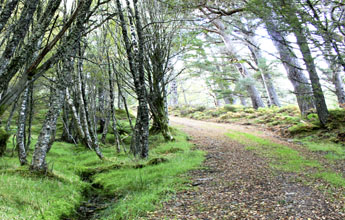
\includegraphics[width=0.5\linewidth]{images/SCP.001.the.spiral.path.jpg}
	\caption*{SCP-001的一部分}
\end{figure}

\bb{项目编号:}SCP-001

\bb{项目等级:}Embla

\bb{特殊收容程序:}SCP-001于[已编辑]州,Site 0就地收容。一道围篱沿著SCP-001的可观察半径筑起。为了安全起见,Site 0随时都需布署五名或以上的武装守卫以防止未经授权的进入。邻近的物理实验室也需随时运作以研究任何异常。

一块刻有提醒标语的金属告示牌应随时维护以保持在最佳状态。任何损伤都需立即回报以进行修补。

\bb{描述:}SCP-001是一条位于林中的环状砾石小径。以逆时针方向行走时,路途会是持续的上坡,就算通过起始点亦然;以顺时针方向行走时,路途的上、下坡数量是相同的,而没有异常。

存取SCP-001的实验记录需五级授权。

监督者议会(Overseer Council)的新成员需阅读\hyperref[chap:DOC-001-05]{文档001-O5}。

\chapter[SCP-001 遗物]{
	SCP-001 Dr. Mackenzie -  The Legacy\\
	SCP-001 遗物
}

\label{chap:SCP-001.the.legacy}

\bb{项目编号:}SCP-001

\bb{项目等级:}Euclid

\bb{特殊收容程序:}SCP-001的所有组件需分开收容于Site Zero中具备环境控制功能的保险柜中。Site Zero的地点为5级机密,唯有O5议会成员才能知悉。

仅允许O5等级人员存取SCP-001本身、其转录以及相关资料,除非经由程序Zero。程序Zero必须在全体O5议会成员一致的直接命令下才能实施,且程序Zero的详细内容只有O5特准的人员才能获取。

\bb{描述:}SCP-001是两(2)个物件与三十三(33)份文件的总称,所有权属于{[}数据删除],又名「管理者(“The Administrator”)」。

SCP-001-01与SCP-001-02分别是{[}数据删除]

SCP-001-03至SCP-001-35的文件混合了手写与打印的格式。这些文件,除了完全没有表现出随时间劣化或破损的情形外,在所有方面都表现正常。对纸张本身年代的化验则得出了不确定的结果。这些文件的内容详列于下,包括{[}数据删除]

{[}数据删除]

{[}数据删除]

{[}数据删除]由于这些物件是基金会成立的推力,同时也构成了基金会的活动准则,因此这些资讯只能在O5议会的直接命令下提供给程序Zero的人员。

\hr

\red{\g{\bb{在O5议会命令下进行5级加密-仅允许阅读}}}\\
\red{\bb{无授权的存取将导致立即处决。}}

\bb{附录001-01:}对SCP-001-01与SCP-001-02的分析

\bb{SCP-001-01}是由未知金属物质所构成的平滑装置,尺寸约22公分宽,30公分高,1.5公分厚。项目的重量与其尺寸极为不符,达8.2公斤。其上有一个小型数位显示器,并且有一个看似是某种钥匙孔的开口。由于没有可见的接缝或紧固件,目前为止,尝试拆解或分析这个装置的尝试都已失败告终。以X光或磁共振扫描SCP-001-01内部的结果显示出不确定的结果,表示装置的内部若不是太过致密以至于无法扫描,就是内部的拓扑结构有异常。

SCP-001-01的能力貌似只有显示两个指标。第一个表现为一种状态或进度条以及数字,目前进度约在23%。另一个指标是一串简单的数位计数器,当前数字为██,███。

\bb{SCP-001-02}是一把与SCP-001-01外壳相同材质的钥匙。目前推定这是SCP-001-01的启动钥匙。

\bb{附录001-02:}SCP-001文件的转录

\bb{SCP-001-03}是管理者的个人日志。SCP-001-04至SCP-001-35在回收时一并夹在SCP-001-03的书页中。

SCP-001-03的片段,第一页:

\begin{scpbox}

我一向很排斥写日记的点子。文件是一回事,但我从来就不知道写下个人思考过程有什么意义。我心中的科学家告诉我,总有一天某人会需要知道整件事情的始末。

\end{scpbox}

SCP-001-03的片段,第三页:

\begin{scpbox}

人们常说,万事起头难。我已经从联邦政府那里取得了足够的资金与人员,并且建立了一个能让我继续研究的组织。{[}已编辑]总统坚持要我交出那个装置以确保安全,但我也把话说的很清楚:我不会交出自己的所有物。

\end{scpbox}

SCP-001-03的片段,第七页:

\begin{scpbox}

不幸地,进度在这几十年间严重落后。我坚持在解答出来前不能重建科技,因为我相信除非我们能一石二鸟,否则只会加速事情的发生。

\end{scpbox}

SCP-001-03的片段,第九页:

\begin{scpbox}

我必须杀掉他们。他们瞒着我偷偷在重建那些科技。我必须在24小时内动身,这处设施从现在起就算毁了。

\end{scpbox}

SCP-001-03的片段,第十五页:

\begin{scpbox}

我不会再犯同样的错误。一想到我为了达成目的而不得不说谎,就令我感到痛心,但我不能再一次承担让他们知道真相的代价了。

\end{scpbox}

\bb{SCP-001-05}貌似是以喷墨印表机印刷的文件,被夹在SCP-001-03的15与16页之间。纸张本身与其他SCP-001的文件以同样的未知方式保存。

\begin{scpbox}

来自管理者办公室的备忘

人类的存在已经延续了数十万年,但直到最近的数千年才真正是我们的时代。我们在信史之前的无数时间中都在做什么?我们瑟缩在洞窟中,用篝火抵御黑夜,畏惧着我们所不了解的事物。不仅是因为我们不了解太阳为何升起,还有巨大而长有人头的鱼、动如活物的石头,以及仅仅看见就令人发疯的怪物。所以我们称其为「天使」或「恶魔」,在它们的盛怒下乞求饶恕并祈祷救赎。

物换星移,它们陨落而人类崛起。整个世界渐渐产生条理。但那些无法解释的事物从未真正走出人们的视野,就像宇宙需要人类所不了解的事物存在一般。

我们不会再退回黑暗、蒙昧、恐怖的夜晚。我们不会被未知所驾驭。我们会走出自己的路。

就算其他人不知情,我们也要对抗黑暗、关住它、不让社会大众看见,这样他们才能继续活在普通世界的美好幻觉里。

\end{scpbox}

SCP-001-03的片段,第二二页:

\begin{scpbox}

他们的脸不断出现在我的梦境中,成千上万。那些人盲目迈向死亡,为了我。

\end{scpbox}

SCP-001-03的片段,第二八页:

\begin{scpbox}

做错了。跟某人坦诚,在离开的前一晚。得用上我仅剩的医疗资源。某方面来说,我希望他瞄准我的脑袋。

\end{scpbox}

SCP-001-03的片段,第四一页:

\begin{scpbox}

这个方程式的解能构成其他解答的架构。我亲手杀死了他们。他们能想到这是出于慈悲而下的手吗?

\end{scpbox}

SCP-001-03的片段,第六四页:

\begin{scpbox}

突然想起,临走以前他们对我说的话,他们说我可能不会看到任何东西,就像睡了一觉一样。他们错了。我亲眼看着他们被疯狂吞噬,现实的界线崩溃粉碎,然后重组,好像它一向如此似的,而我看到整个过程。

\end{scpbox}

SCP-001-03的最后片段,第六八页:

\begin{scpbox}

终于完成了。方程式已经完备,数字也齐全了,但再一次,这个结果来得太晚了。这个小组没有时间建构解答,而我必须再一次放弃基金会。但这次我有足够的知识,确保不会再有人遭受同样的命运。

\end{scpbox}

\bb{SCP-001-34}是一份破损的手写文件,夹在SCP-001-03的封面与首页之间。

\begin{scpbox}

敬启者:

首先,我为我所做的一切道歉。单单我存在于你们的世界这件事,可能就毁灭了你和你所知悉的一切。如果你现在持有,而且正读着这份文件,那我很可能已经死了。即便如此,我也会顺手毁了这份证据,而这表示我也失败了。也就是说,我的责任现在全都落到你肩上了,而你的命运与你世界的命运现在都操之在你。

我并非诞生在你们的世界,我是来自另一个现实,行走于平行宇宙之间的旅行者。我从哪个年代来并不重要;我在路途上了解到,时间流逝对于跨宇宙移动而言是没有意义的。重要的是,在我原本的宇宙中,人类的文明发展到了一个极致。我们汲取星辰的能源,学到如何操纵现实本身的架构。我们能按照自己的需要折叠时空,甚至以医学和科技征服了死亡。我们以为自己掌握了命运。

当我们了解到凡事都有代价时,一切都已经太迟了,我们不仅会失去我们所珍视的一切,甚至殃及他人。操弄宇宙结构的结果,使现实撕裂扭曲,当现实的残片开始泄漏时,我们还没有发现这是多重宇宙崩溃的前兆,然后反馈开始出现在我们自己的宇宙,已然无法阻止。

我们勉强在卷入崩溃之前,启动了最后一项保险。我们集合了残存的知识,并牺牲了自己的世界将一个人送到下一个世界。这无法修补已经造成的伤害,但能为我们争取时间,找出阻止现实崩溃的方法,这个人就是我。

如果你还没有找到,那能佐证我言论的事物很快就会开始进入你的世界。其它破碎宇宙的碎片将如玻璃上的雨水一般滴漏进来。那是与你的理解相违悖的东西;没有明显意义,却固定在时空里的物体;无法被你任何手段摧毁的事物;那些能逼疯人的存在,会让你所重视的所有理论都作废。

我所携带的,是无数世界所留下的最后遗物。在这些书页中所描述的方程式与科技带着一份阻止崩溃的希望,一份巨大代价所换来的希望。是所有牺牲与被牺牲的宇宙一路走来的,血淋淋的轨迹,只为了让剩下的人不再重蹈他们的覆辙。在我写下这段文字时,它们已经接近完成了,但时间永远与我作对。如果我无法亲眼看着这份艰苦的任务完成,那就只能靠你了。

祝好运,\\
{[}数据删除]\\
管理者

\end{scpbox}

\bb{SCP-001-35}是一份手写的文件,被夹在SCP-001-03的末页与封底之间。SCP-001-35的字体与SCP-001的其他文件均不符。

\begin{scpbox}

{[}数据删除]:

这个,就是我们的文明曾经存在过的唯一证据了。没有人真正知道当你启动保险时会发生什么事情。有些人说使用所造成的反弹会立刻撕裂我们的宇宙中剩下的部份。其他人说使用它的力量仅仅会使崩溃加速数百倍。无论哪一种方式,都只是一眨眼的事情。当你在你的目的地醒来时,我们的家园早已荡然无存。

你已经知道这个装置只能承载一个人,而第二个小队在你离开时已经准备就绪。我只希望我们帮你争取的时间,能让你找到阻止这场灾难的方法。不然的话,这个装置也能持续记录本地现实的崩溃程度,以及装置被启动了几次,我们这么做,或许有点虐待狂倾向吧?

当你读到这里,我可能已经死了。我很抱歉,但你一直以来就是比较坚强的那个。我没办法从容面对自己的终结。在没有你的情况下。

我爱你。

\end{scpbox}

\bb{附录001-03:}SCP-001-36\\
SCP-001中的文件证明SCP-001-36的存在,一件电子设备或是详载着与SCP-001相关的科技和数学资料的大量文件。SCP-001-36目前下落不明。


\chapter[SCP-001 数据库]{
	SCP-001 S. Andrew Swann - The Database\\
	SCP-001 数据库
}

\label{chap:SCP-001.the.database}

\bb{项目编号:}SCP-001

\bb{项目等级:}Keter

\bb{特殊收容措施:}目前尚未找到一种方法可以收容SCP-001而不带有可能引起ZK级现实崩溃和其导致的可观测宇宙毁灭的风险。(参考:监管协议ZK-001-Alpha)当前的措施被限制在对关于SCP-001信息的绝对封锁上。有关SCP-001的性质或对其描述的信息都不得被提供给任何人,除了唯一的一名O5级指挥长官(目前是O5-█)以外。一切收集到的关于SCP-001的数据都须被以【删除】的方式进行加密存储,且密钥需被分为三部分。每一名O5级指挥人员都需记忆且只可记忆密钥的三分之一。数据只可以被在仅供O5级指挥长官阅读的非联网的视觉终端上面被解密,并且需要全体O5级指挥人员的一致同意才可进行。

由于谍报、心灵感应、研究或者【删除】导致的关于SCP-001的数据泄露必须被基金会不惜一切代价阻止。O5级指挥长官,作为唯一一位有权限掌控SCP-001知识的人员,对收容措施拥有最终裁定权。

在正常任务中接触到关于SCP-001数据的2级或以上的基金会员工可在接受询问之后被处以A级记忆删除处理而不是被处决。此类事件的处理由O5级人员视情况而做出决定。

\bb{描述:}【数据删除】

\bb{附录:}收容日志001-Alpha

\begin{scpbox}

\bb{日期:}01\slash 12\slash 19██

\bb{事件:}文件出现在互联网站点【删除】。服务器已被夺取且文章作者于【删除】被追踪到。制造了一起被伪装成煤气泄露的爆炸。没有监察到关于文件的进一步宣传。

\bb{日期:}03\slash 31\slash 19██

\bb{事件:}██████ ████的一份电影剧本包含可能的泄密信息和图片。剧本原作者已被【删除】。探员成功地用一份不含有【删除】内容的剧本替换了原剧本。电影以███ ██████的名字上映并在周末首映获得2700万的票房收入。\footnote{\bb{译注:}这部电影是黑客帝国(The Matrix),上映时间和首映票房与描述相吻合。}

\bb{日期:}06\slash 19\slash 19██

\bb{事件:} 畅销书作家█████ ████提供给了【删除】一份描述【删除】的小说大纲。对作者的刺杀未能成功,导致目标高调地住院治疗。O5授权允许只用A级洗脑来阻止可能引起的进一步关注。大纲被回收并销毁。\footnote{\bb{译注:}这位作者是著名恐怖小说家史蒂芬·金,史蒂芬·金确实在1999年6月19日遭到过一次车祸袭击。}

\bb{日其█:}o5\slash 2█\slash 20█z

\bb{事█牛:}基nAt金会on石█sea九e█\%20发scov\\
\tred{\%5B数ttt据删xPu██ge余\%5D}

\tred{\%5B数ttt据删xPu██ge余\%5D}

问问你自己你是否想要知道。

如果答案是不,那么现在你不要继续读下去了。如果你现在离开并且将这未授权的文件汇报给你的上级,表现得痛心疾首,并且声称你只读了这一小段的话,你大概能在接受A级洗脑之后留下你的小命。当然,如果你很幸运而且那些O5的老大们当时恰好不那么多疑的话。

所以你想要知道SCP-001到底是什么?第一个能想到的答案是它是一个占位符,一个为了首要目的理论规划,和我们每天处理这些不正常玩意儿的最终原因。SCP-001就是\bb{\ii{为什么}}我们必须去应付打不死的爬虫、不断膨胀的房间、多维的红色粘液池和违反物理法则的消费品。当然,考虑到这所有的一切——既致命又疯狂的玩意儿——都缺乏固有特征而又自相矛盾,大部分的研究者都确信没有办法找出它们共有的法则,更不用说找到其共同的起源了。

他们错了。

交互测试不被接受有很多原因,而O5们甚至是鄙视那些将不同的SCP进行牵强附会的\ii{交互}的行为。O5们不想让任何一组成员同时研究稍微多一点的这些东西,这都是由于当基金会\ii{试图}找出一个SCP的大一统理论时他们所发现的东西。那些研究现在大部分都已经遗失了。001-Alpha地点已经被拆除,从档案中被抹掉,员工们被洗脑和调走。除了我之外谁都没有留下,而我也不会知道这一切,如果不是因为我有着不信任基金会的服务器的习惯并且私藏了一份令O5们惊慌失措的个人档案的话。

我是一个001-Alpha号地点的数据分析员\ii{【给O5级指挥人员的备注:别费劲找我,我完成了你们的目的,001-Alpha地点的所有原员工的身份都已经被从记录里\bb{完全}的抹掉,现在你们也不会知道更多事情了】}并且参与了第一次也是唯一一次试图合并基金会所有SCP数据的尝试。我的任务是负责数据的完整性。不管你们觉得这到底有多离谱,相信我,它实际上要更糟。

忘了那些模因的SCP吧,或者是那些定义自己描述的,或者是那些只存在于信息空间里并且在数据库里造成破坏的东西吧。对在基金会的网络中工作的人而言,现有的这些SCP没什么特别,只不过是数量多少的问题而已。真正可怕的,是数据库当中那完全不可知也无法解释的改变。

抱歉,我错了,尽管我实在忍不住这么想。它不是当\ii{现实}发生变化时\ii{数据}做出的相应改变。我对于我们使用的软件的内部所知甚少,但是我知道里面有一部分遁入了我们所认为的“现实世界”当中。并且,最初所有人都认为审查追踪到的结果只是某种BUG而已。但是,明显可以看出这软件的性质,即它和那些影响叙述的SCP们之间的有意识的孤立,使得它可以去记录一些远更为重要的事情。

那是你们、或者O5们、甚至是我们处理的大部分SCP们所看不到的,但是基金会——直至整个宇宙——处在持续的现实不稳定变化中。SCP档案令人不安的从我们的数据库中出现和消失,而档案所提到的SCP,从各方面,也和档案一同出现和消失掉。不仅仅是SCP,是人员,整个地点甚至是基金会几十年之间的历史都会被重写,且无法捉摸其规律。而我们自己的记忆,以及所有的研究都会确认“客观现实”和数据库里当前的情况一致。

有一个研究员告诉我说我们好像在寻找某些拥有像SCP-140那样的东西,只是更大一点而已。

对的。某些\bb{非常}像SCP-140的东西,并且是\bb{无穷}大的。

我不知道谁做的分析,说不定是我做的。如果她不知道自己的发现的话可能会更快乐一些。但是她看着那些消失的和出现的事物,那些隐约的记录的改变,并且她找到了那形式和趋势,朝着黑暗、朝着有条理的叙述,朝着一个计划……

每一个在基金会工作过一段时间的人都会知道我们生存的宇宙是一个相当混乱的地方。我们仍然相信上帝对祂的造物保持着矛盾的态度。

但是我们最终发现确实有一个上帝,那就是SCP-001。

而那是一群可怕的作者们。

\end{scpbox}

\bb{附录:}紧急收容协议ZK-001-Alpha \bb{仅供O5人员阅读}

\tred{输入密钥}

\tred{密钥正确}

备注:收容协议001-Alpha带有一定的导致ZK级现实崩坏事件的可能性。只可在世界末日情景或者是基金会面临毁灭的情况下被授权使用。

在001-Gamma地点进行的研究分析和叙述了SCP-001的改变对可观测宇宙引发的影响。结论是SCP-001由多个和人类认知形式相同的个体组成,并且因此这些个体会受到模因效应的影响。由于先前的实验显示SCP数据库会引发信息反馈,我们研发了一种可能的攻击或者控制的手段。协议ZK-001-Alpha,当启动的时候,会通过软件病毒将多种模因作用剂导入SCP数据库,并且通过可观测的数据反馈,将SCP-001暴露于这些作用剂的模因效应当中。ZK-001-Alpha协议包含三个阶段:

\begin{enumerate}
\item 导入引发冷静和友善的模因作用剂
\item 导入引发睡眠、昏迷或紧张的模因作用剂
\item 导入引发死亡的模因作用剂
\end{enumerate}

鉴于SCP-001的性质和我们对它所知甚少的相互作用,目前尚无法安全的测试ZK-001-Alpha协议,并且仍然未知在没有SCP-001作用的情况下宇宙是否能继续存在。


\chapter[SCP-001 基金会]{
	SCP-001 Scantron - The Foundation\\
	SCP-001 基金会
}

\label{chap:SCP-001.the.foundation}

\begin{figure}[H]
	\centering
	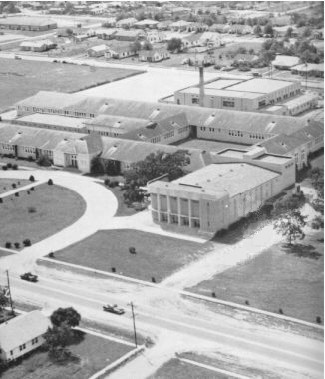
\includegraphics[width=0.5\linewidth]{images/SCP.001.the.foundation.jpg}
	\caption*{CA3的空照图,摄于最初发现后两个月。}
\end{figure}

\bb{UIU档案 0041:}位于██████, ██的变异高中校舍(Confirmed Anomaly 3,已确认异常3号)

\bb{项目等级:}53(高侵入性、未知能力、未知性质)

\bb{特殊收容协议:}\dd{已确认异常3号(CA3)需被高于30尺的带电铁丝网所环绕,并由美国陆军第█████排守卫。任何关于CA3内部的影像资料都需尽快删除,且所有目击者都将被无限期囚禁。}

在所有情况下都不允许人员进入CA3,或与居住其中的人员沟通。但在任何时候曾经进出CA3的人都应被囚禁与审问。

由于控制项目的一个或多个实体所拥有的未知能力,对CA3的直接军事突击已经被证实是不可行的。

\bb{笔记:}\ii{这是一份摘要,不包含所有关于CA3的资讯。对CA3的详细资料请参阅UIU档案0042至0218} - ██████主任

\bb{已知资讯:}特异事故处在1954年九月五日警觉到CA3的存在,当██████████高中的学生报告他们的校舍内部发生了前所未有的变化。

在发现的当下,CA3表现出数个-若非原本就存在的-异常性质:

\begin{itemize}
\item 设施内几乎所有墙壁都被钢筋混凝土所替换,某些房间则以其他材质建造,原因不明。所有对外的窗户都从内部被掩盖。
\item 所有课桌椅、个人财物、课本,或其他公立高中应有的物件都消失了。保险柜仍存在,但尺寸明显缩小,且是由不锈钢构成。
\item 所有房间与设施的格局、位置与尺寸都与学校原本的蓝图不符。且房间内部经常出现看似随机的修改,被改变的房间数量仍旧不明。
\item 发现了不少于七台的计算机,每一台都使用最先进的磁芯内存。在被分类为已确认异常之前,██████████并没有计算机。计算机内的所有资料都无法存取,且机器本身都被螺丝固定住。
\item 礼堂被大面的钢墙阻挡而无法进入。对这个阻碍进行搬移或破坏的尝试皆以失败告终。墙壁与礼堂本身的规模与用途不明。
\end{itemize}

一支被送入CA3内部以进行完整调查的小队(CA3-O5小队)没有返回,而负责寻找前一小队的第二支队伍也是(CA3-06小队)。该设施目前被封锁,等待新的收容措施。

\bb{更新:}在最初发现的二十三天后,守卫回报CA3发出「白噪声\footnote{\bb{译注:}White Noise,在各频率上功率都相等的“干扰”或者“噪声”}」,越接近礼堂噪声越大。五小时后,白噪声停止,但CA3内部能听见谈话声。

在深入调查之后,发现建筑内部现在包含了大量人员,所有人都看似漫无目的地在设施中游荡。值得注意的是,每个个体在外观上都与CA3-06的队员一致,但CA3内部的居民数目远超过CA3-06。囚禁或互动的试图因{[}机密]而失败。没有发现CA3-O5小队的十二名成员。此外,CA3的内部规划与前次调查也有明显差异。其中的运作机制尚未明了。

进一步的调查显示,大部分(或全部)产生出的物件本身都具有异常的性质。一部分的CA3-2开始看守这些物件(通称为CA3-3)或对其进行各种实验。

\bb{更新:}在前次调查的两天后,三名雷同的武装「守卫」出现在CA3的入口附近。由于这些守卫能无视伤害或武器等级地制服所有派往CA3的队伍,无法进一步探索建筑。

\bb{笔记:}在守卫出现前两天搜集到的报告指出CA3-2遵循标准UIU程序来处理礼堂中出现的物件。他们对UIU标准程序的知识与CA3-O5小队一致。

\bb{更新:}在UIU追踪CA6的过程中,两名与特工Dixon(CA3-06的成员)相同的人从路边的车辆中出现并强行掳走了CA6,将他拖入车中扬长而去。往后八个小时对车辆的追踪发现他们直接驶往CA3。在抵达的时候,守卫迅速开关前门让车辆通过。CA6没有再被寻获。

\hr

\hr

\bb{UIU档案0042:}CA3发出的讯息

1965年五月15日,以下讯息以摩尔斯密码发送至标准UIU通讯频道上。敏感资料已被删改,并将每个「句子」加以编排,讯息本身并未更动。

\begin{scpbox}

你好!我们是O5议会而且我们(控制、收容、保护)我们的行动已经为你们所知而且很高兴能做朋友。以前能当你们的一份子很好但最好是有更充足的资源(更多的资源)我们会控制住收容。我们对于守卫与囚禁的行为,在此表示诚挚的歉意,我们需要保障人员与秘密:同时也对时间上的延宕道歉,无线电讯号被一或二个SCP所阻挡。预期在短时间内会有扩张,因为我们需要礼堂以外的空间(尚可但不佳)

\end{scpbox}

八小时后,收到下列讯息:

\begin{scpbox}

扩张了!█████████联邦大楼现正运作中,需要博士守卫D人开始招募!寻找异常而且未来可能进行国际行动,研究当然可行;但跨国活动可能需要数周。此外我们O5都知道(抱歉没有O6)虽然很难探查,但媒介礼堂不是█████!再会并祝你们好运。

\end{scpbox}

更进一步的资讯参阅UIU档案0███:位于█████████, ██的变异联邦大楼(已确认异常10号)


\chapter[SCP-001 三十六]{
	SCP-001 Djoric/Dmatix - Thirty-Six \\
	SCP-001 三十六
}

\label{chap:SCP-001.thirty.six}

\bb{项目编号:}SCP-001

\bb{对象类别:}人形

\bb{威胁级别:}绿型(Green)|部分情况红型(Circumstantial-Red)

\bb{收容等级:}Euclid

\bb{特殊收容措施:}SCP-001个体将被收容于标准人形收容间中。任何情形下禁止将多个SCP-001个体收容于同一站点、允许其以任何形式发生互动或是得知该群体其他成员的任何相关信息。 被分派到任何单个SCP-001个体的所有人员不得得知其他SCP-001个体的存在或它们之间的联系。

除了经由批准的测试外,SCP-001项目将不会与任何其他异常物品进行直接接触。

修订于██\slash ██\slash 20██:O5特别指令A-1130-X

由于SCP-001-05死亡事件的后果,特此禁止将SCP-001项目用于任何异常项目的无效化上。必须尽全力保证SCP-001项目的生存和无恙。对SCP-001项目的寻找和收容将被最优先考虑。一但死亡事件发生,必须以最快速度开始执行衔尾蛇协议(Ouroboros Protocol)。

\bb{描述:}SCP-001是一组36个人形个体的集合,分别命名为SCP-001-01至SCP-001-36。在SCP-001项目之间没有任何可见的在种族、性别、年龄或宗教信仰上的统一模式。

每个SCP-001个体自身展现不出任何异常性质。但是,任何异常物品、实体或特性在靠近SCP-001个体时都会较其原本特性发生极大程度改变:一般而言,这会导致其异常特性的削弱或是彻底无效化。那些没有被无效化的特性会被变得与具有类似特性的对象相一致。所有这些效应都是瞬间的且会在没有任何来自个体的接触下发生。这些效应的范围会在多个SCP-001个体相互靠近时扩大,其变化的强烈程度也是如此:多个SCP-001项目有能力在不察觉到其存在的情况下将对象的异常效应无效化。

所有的SCP-001个体似乎都本能地了解其他SCP-001个体的相关信息,一般是这个群体的总人数和其他大约二至三人的详细信息。这种了解是模糊的,这也给锁定未被收容的个体带来了困难。

SCP-001个体的死亡会导致多种异常实体和现象在其死亡地点显现。此类显现的严重程度将会使传统收容措施根本不能实行,并造成严重事故和一系列相关破坏。被收容的SCP-001个体宣称这是因为那些死亡个体的缺失“让那些东西穿过来了”,而且随着时间推移还会有更多更严重的的事件。此外,已收容个体还宣称任何一个死亡个体都会被一个拥有相应特性的新生儿代替,但当前尚没有这样的个体被发现。

要了解SCP-001对物品造成的值得注意的变化的列表,参看文档001-EX。对所有无效化的完整列表可以在文档001-N找到。

\bb{附录-01:}

已知的SCP-001成员如下:

\begin{longtable}{m{0.08\linewidth}m{0.13\linewidth}m{0.08\linewidth}m{0.08\linewidth}m{0.14\linewidth}m{0.24\linewidth}}
\hline
编号 & 人种 & 性别 & 年龄 & 当前状态 & 备注\\
\hline
\endhead
\hline\multicolumn{6}{r}{\small{接下页}}
\endfoot
\hline
\endlastfoot
SCP-001-01 & 犹太裔德国人 & 男 & 94 & 已收容 & 当前处在人工抑制中以防止其死亡。在其左臂上印有数字表示的身份识别。\\
SCP-001-02 & 泰米尔人 & 女 & 88 & 已收容 & 收容时正处于怀孕中。孩子平安出生,当前正处在基金会观察中。\\
SCP-001-03 & 不列颠人 & 女 & 91 & 已收容 & 个体被记录是一名于1943年死亡的英国随军护士。\\
SCP-001-04 & 中国汉族人 & 男 & 97 & 已收容 & 一名全真教道士,第一个向基金会透露与其他个体相关信息的个体。\\
SCP-001-05 & 普什图人 & 男 & 101 & 死亡 & 个体于收容期间死亡。详情参见事故报告001-05-EX。\\
SCP-001-06 & 意大利人 & 女 & 39 & 未收容 & 最早被回收于布达佩斯的一处旅馆中。八天后在SITE-90的一次收容失效中逃跑。当前位置未知。\\
SCP-001-07 & 波兰裔阿根廷人 & 女 & 52 & 未收容 & 被GOI-16“地平线倡议”控制。\\
SCP-001-08 & 俄罗斯人 & 男 & 5 & 未收容 & 被未知个人或组织控制。没有发现其家庭成员。\\
SCP-001-09 & 土著澳大利亚人 & 女 & 31 & 未收容 & 被GOI-16“地平线倡议”控制。\\
SCP-001-010 & 非裔美国人 & 男 & 28 & 未收容 & 被GOI-16“地平线倡议”控制。\\
SCP-001-011 & 尼日利亚人 & 男 & 45 & 已收容 & SCP-001-011的家人在对其进行回收的过程中出现。他的长子不顾其反对对基金会人员进行武力抵抗,被杀。其余家庭成员已接受了A级记忆删除。\\
SCP-001-012 & 阿拉伯人 & 女 & 14 & 死亡 & 在回收过程中被GOI-03“混沌分裂者”成员杀死。详情参见事故报告001-012-RC-EX。\\
SCP-001-013 & 韩裔美国人 & 女 & 未知 & 未收容 & 尚未成功回收。\\
SCP-001-014 & 纳瓦霍人 & 男 & 23 & 已收容 & 在对象和\hyperref[chap:SCP-1295]{SCP-1295}联系后被基金会人员回收。详情参见文档001-EX。
\end{longtable}

\bb{附录-02:}SCP-001-01到SCP-001-05最初于██\slash ██\slash 1944在一次由HMFSCP对耶路撒冷地区发生的疑似奇迹和其他异常事件进行的调查中被回收。SCP-001-01到SCP-001-05被发现时由三人照看,此三人分别被归为POI-1458,POI-1459和POI-1460。上述三人可能与GOI-16“地平线倡议”有联系,并有可能参与了该组织的创立。

回收尝试因HMFSCP的内部争斗被妨碍。SCP-001-01在交火中严重受伤,但还是被成功稳定住并和其他个体一起被回收,并被保护主义者派别控制。负责保护这些个体的那些人员在交火中逃走,之后再没有被逮捕到。

\bb{采访记录001-11-02}

下面对SCP-001-05的采访记录于██\slash ██\slash 19██。

\begin{scpbox}

Dr. ████████:你上次说你有一个特别的使命。你能解释一下吗?

SCP-001-05:我在这里是为了把事情纠正到位。

Dr. ████████:请继续。

SCP-001-05:这世界是破损的,博士。我的兄弟姐妹和我来到这里是为了将它治愈,我们集合起来并为将要到来的做好准备。进程本已经开始推进,但很遗憾出现了一些波折。

Dr. ████████:请解释一下。

SCP-001-05:{[}SCP-001-01],他本是那个负责把所有其他人集合起来的人。 但因为他现在正在生死线上挣扎,这个任务落到了我们身上,但我们只能瞥见一小部分其他人。不过这本来也足够了。

Dr. ████████:你不为他的安危担心么?

SCP-001-05:死亡只是将要做的事的另一部分。没什么好担心的。

Dr. ████████:真是令人赞叹的处事态度。你是怎么发现自己的使命的?

SCP-001-05:我做了个梦。预兆,预言,幻象,随你怎么叫它吧。它在我脑海中种下了一颗种子,你可能会把这叫做一种直觉。那是在我见到 {[}SCP-001-01]的后一天。

Dr. ████████:你能描述一下那个梦吗?

SCP-001-05:那里有个男人,穿着很华丽,看起来像个国王或者皇帝。他不停地说“裁缝在哪?我的裁缝在哪?”,同时来回踱步。每一次他问出这个问题,另一个声音就会回答到“他就要来了,他就在眼前”。但是那个他并没有到来。男人变得越来越沮丧,突然一群飞蛾扑到了他身上,开始啃食他的衣服。随着越来越多的飞蛾扑到他身上,他的长袍开始磨损、腐坏,有些飞蛾甚至开始咬他的皮肤。但是突然,门开了,来了不止一个裁缝,而是许多个,由全王国最杰出的裁缝领导。国王万分欣喜,因为他明白,他们能从这群想毁灭他的飞蛾中将他解救。他找到了我,而我跟随他。

Dr. ████████:如果你不用这种戏剧性的措辞,这就是说当你们所有人聚在一起时,这个世界就会走向终结,对吗?

SCP-001-05:{[}轻笑]博士,这个世界已经终结了。这只是最后一战。这世界的时辰已经到了而且已经过了,它只会被拉扯得越来越薄,直到有一天除了飞蛾什么都不会留下。但是,还是剩有一些时间。我们终能靠自己找到彼此。

Dr. ████████:那这会在什么时候发生?

SCP-001-05:在那平静的日子(Quiet days),博士。平静的日子,还有和平。

\end{scpbox}

\bb{事故报告001-05-EX}

\tred{+ 仅限授权人员查看}

\tred{- 安保模因:WHAT SWORD SHALL YOU CHOOSE}

\bb{日期:}██\slash ██\slash 19██

\bb{地点:}Site-128(坐标██-██.█-██.█)

\bb{事件类型:}LK(局部危机)

\bb{描述:}事件在SCP-001-05死亡的瞬间,当地时间22:12发生。驻扎于Site-41,Site-98和Site-203的所有MTF小组立即展开回应。对Site-128内所有物品的清除协议于22:15被批准。

\bb{产生异常}

\begin{itemize}
\item UAP-████ - 近似由粘土构成的自我复制实体,一旦接触到有机脊椎动物,实体会整个包裹住宿主,控制宿主的行为。若周围没有宿主,实体会平铺伸展或聚合成大团物质。
\item UAP-████ - 长有八只羽翼、带有鸟类和头足类特征、展翼后长70M、高45M的实体。同时显现出大群外表类似乌鸦或渡鸦的实体,每个长约3M。
\item UAP-████ - 一系列共109个巨型立方八面体,每个宽约1M。以每个对象为中心半径20M范围内空气温度提升到超过250度。受影响区域会在脱离影响范围后立即冷却下来。对象能以大约25KM每小时的速度飞行。
\item 9次被记录的3级生物复活情景。
\item 大范围的市民自发仪式性食人报告。
\item 从最初事件站点延伸出约110KM范围内的异常天气模式。降雨中含有大量致命病原体,包括扎伊尔埃博拉病毒(\ii{Zaire ebolavirus})、大肠杆菌(\ii{Escherichia coli})和重型天花(\ii{Variola major})。
\item SCP-1348消失. 参见文档001-EX。
\end{itemize}

\bb{回收尝试:}衔尾蛇协议于22:23实施,在21:00完成。协议以97\%有效率被执行。

\bb{基金会伤亡:}1350\\
\bb{物品遗失:}27\\
\bb{预计平民伤亡:}10000

\bb{事故报告001-012-RC-EX}

\tred{+ 仅限授权人员查看}

\tred{- 安保模因:THROUGH THE LONG NIGHT}

\bb{日期:}██\slash ██\slash 20██

\bb{地点:}{[}已编辑],东萨莫色雷斯伊斯兰共和国(Islamic Republic of Eastern Samothrace)

\bb{事件类别:}LK(局部危机)

\bb{描述:}对SCP-001-12的回收被定在当地时间07:31执行。对象勉强地表现出合作。在07:43,来自GOI-03"混沌分裂者"的特工对回收小组发起袭击。SCP-001-12在事件中受重伤, 还有特工████和████████。SCP-001-12这时开始语无伦次,表现出言语不清的症状:对对象当时的胡言乱语的记录如下:

\begin{scpbox}

它们饿了,你看…又咬又叮又嘎吱嘎吱嘎吱嚼…不新鲜的食物总比没有好,明白了吧?它们非常饥饿,而且会越来越饿。

\end{scpbox}

回收小组在08:15受到第二次攻击,SCP-001-12死亡。

\bb{发生异常:}

\begin{itemize}
\item UAP-████ - 高约50M,长200M的半无定形四足实体,能抵抗常规武器攻击。
\item UAP-████ - {[}资料删除]
\item 由大量蛆产生的自发性人体崩溃(物种未知)。
\item {[}资料删除]
\item {[}资料删除]
\item 突然出现的洪水,由2\%巧克力牛奶、原油、鸡肉汤和兔粪便组成。
\item SCP-1348再次出现. 值得注意的变化参见文档001-EX。
\end{itemize}

\bb{回收尝试:}监督者议会于08:17批准核武器调度。衔尾蛇协议于08:46实施,于07:30完成。协议以61\%有效效率被执行。

\bb{附注:}考虑到因衔尾蛇协议实施过程中的瑕疵造成的现实不稳定,东萨莫色雷斯伊斯兰共和国已被归类为\hyperref[chap:SCP-1173]{SCP-1173}。

\bb{基金会伤亡:}8\\
\bb{预计混沌分裂者伤亡:}25\\
\bb{预计平民伤亡:}175,000

\bb{文档001-EX}

\tred{+ 仅限授权人员查看}

\tred{- 安保模因:WE SAW THEM WALK ON CLOUDS OF MEAT }

\ii{实验记录SCP-001\slash 361}

\bb{前言:}由于SCP-001可能具有亚伯拉罕系根源,并可能对与其起源相近的宗教背景异常事物产生潜在的影响,需要进行一个确认其影响是否存在更广泛基础的测试。\hyperref[chap:SCP-361]{SCP-361}因其危险系数低、属于非亚伯拉罕系的宗教项目且其效应易被观察而被选中进行测试。

\begin{scpbox}

\bb{<记录开始>}

SCP-001-02被引导以一块羊肝碰触SCP-361。

\bb{SCP-361:}欢迎来到HarusCo! 我们-噢,怎么是你。

\bb{SCP-001-02:}看起来是这样。

\bb{SCP-361:}好吧,如果是你在召唤,这就意味着…该死。时辰到了。

\bb{SCP-001-02:}是的。

\bb{SCP-361:}好吧,我们本来觉得我们应该能看着它到来的。来往最近已经变得很少了。也许是时候出发了。

\bb{SCP-001-02:}你们将会和我们一起去往那里,就在一切再一次回归秩序时。

\bb{SCP-361:}就算你有能耐这么做吧。好吧,孩子,我们也许是时候说再见了。我们的老大和你的老大并不总是有一致的看法,但是总得说来我们还是一起度过了一段愉快的时光。那真的很愉快。

\bb{SCP-001-02:}你会去到那里的,我保证。

\bb{SCP-361:}而我们也绝对不曾怀疑你相信这一点。在另一边再见,孩子。或者,不见。

\bb{SCP-001-02:}呵. 我都记不得上一次有人叫我“孩子”是什么时候了。

\bb{<谈话结束>}

\end{scpbox}

\bb{结语:}在测试001\slash 361后,SCP-361停止活动。所有试图引起其原本常规反应的尝试都只收到了一种类似不连贯拨号音的声音。

\ii{实验记录SCP-001\slash 738}

\bb{前言:}\hyperref[chap:SCP-738]{SCP-738}由于可能的关联性被选中进行测试。SCP-001-03没有给出实体(下文称为SCP-738-4)的外貌描述。

\begin{scpbox}

\bb{<记录开始>}

\bb{SCP-738-4:}好吧,看看谁来了!最近过的怎样?我能为您做点啥?

\bb{SCP-001-03:}传个信,Jack。下一次你回去的时候,告诉所有人做好准备。契约即将终止。

\bb{SCP-738-4:}你在唬我吧?这真不是某种骗傻瓜的烂把戏?

\bb{SCP-001-03:}绝对不是。

\bb{SCP-738-4:}真的是时候来点大事了,嗯?我\ii{操}他个烂逼居然已经这么久了!!你猜怎么着?对你,免费。这次我请客。这可完全是出于我那颗枯萎黑心的善意。

\bb{SCP-001-03:}好吧,也许不是那么黑。

\bb{SCP-738-4:}{[}狂笑,猛敲桌子]你这是要把我乐死在这里!看,这就是我喜欢你的原因:你总是带来欢笑。

\bb{<记录结束>}

\end{scpbox}

\bb{结语:}由SCP-738-4留下的契约上写着“本次店家请客。—X”。SCP-001-03没有对为什么称SCP-738-4为“Jack”作出解释。SCP-738当前再被使用时没有展现出异常效应并已被归类为SCP-738-N。

\ii{实验记录SCP-001\slash 1295}

\bb{前言:}于██\slash ██\slash ████, 18:03,当所有四个\hyperref[chap:SCP-1295]{SCP-1295}个体正要离开餐馆的时候,一个人突然叫住了它们,后来此人被编为SCP-001-014。由于对SCP-1295的收容措施不允许基金会人员在场景中于SCP-1295发生直接接触,作为代替对对话进行了记录。

\begin{scpbox}

\bb{<开始记录>}

\bb{SCP-001-014:}先生们,我能占用你们一点时间么?

\bb{SCP-1295-4:}哎哟喂,看看那谁总算是来了!小伙子,你知道我们等你现身有多久了?什么东西耽误了你这么久?

\bb{SCP-001-014:}我很抱歉。我只是最近才发觉我的职责所在。

\bb{SCP-1295-1:}噢,别在意,孩子,Dwight就是有点语无伦次。他其实是想说能见到你真的是太好了。

\bb{SCP-1295-2:}赞成。坐在这一点都不舒服,还只能吃一大堆水果酥皮饼直到腻了为止。是时候回到正事上了。

\bb{SCP-001-014:}那正是我来此的目的。你们骑乘的时刻就要来临。我被授予任务来通知你们并让你们开始准备。我被告知你们知道该做什么。

\bb{SCP-1295-3:}我们当然知道,我的孩子,我们当然知道。不是我自夸,没有人比我们知道的更清楚。

\bb{SCP-001-014:}请允许我提醒你们,我们生活在不同的时代里。这个任务需要的是外科手术刀,而不是大砍刀。此时此刻,你们需要做的温和一些。

\bb{SCP-1295-1:}该死. 我就怕你会说这个。

\bb{SCP-1295-4:}别担心。我们会做的像随人差遣一样温和。我怀疑在所有这些完成以前我们会再见面的,我的孩子。你得自己小心。{[}对SCP-1295-1到3] 来吧,伙计们!时间不等人,我们还有一大堆事要准备!骑行吧!

\bb{<记录结束>}

\end{scpbox}

\bb{结语:}所有四个SCP-1295个体接着离开了餐馆。在他们离开后,基金会人员拦住SCP-001-014并将其逮捕,没有造成更多事件。从这次谈话后再没有SCP-1295回到这家餐馆或是被人目击到。

\ii{实验记录SCP-001\slash 1348}

\bb{前言:}在SCP-001-05死亡后,Site 87的考古学收容单元(Archaeological Containment Unit)经历了一次DK级(维度改变)事件,站点凭空消失并变得不可从外部进入或通信。在SCP-001-12死亡后,Site 87回到了原来的位置。站点一回归,移至探索小队被立即派去调查\hyperref[chap:SCP-1348]{SCP-1348}的收容状况,并发现其运转发生了如下变化:

\begin{itemize}
\item 所有在站点消失时在场的基金会人员全部消失,一起消失的还有他们的个人设备、电子仪器和食物配给。
\item 5个新的SCP-1348-1个体出现在SCP-1348的内室中。不像之前被发现的SCP-1348-1-E,这些新个体看起来完全健康。上述个体被发现在进行SCP-1348-2仪式。
\item 被编为SCP-1348-2的仪式发生了改变,这似乎是因为之前提到的SCP-1348-1的出现。由SCP-1348-1进行的修改版SCP-1348-2缺乏之前版本所具有的模因效应。由于SCP-1438-3的帷幕当前已经永久性打开,修改过的SCP-1348-2的用意当前尚不明确。
\item 被编为SCP-1348-3的内室发生了值得注意的变化。室内原本完全是原始闪米特风格的装饰现在包括了来自多种文化风格的图案,包括中美洲、原始印欧和南极风格,此外这些图案明确地起源于距SCP-1348可能建造时期很长一段时间后的某些时期。
\item SCP-1348-3中心的帷幕现已永久性打开并被发现空空如也,除了一些刻在帷幕内部的阿姆哈拉语蚀刻:“他已经受了太多太多的苦难,已经把这世界的重担扛在他破损的背脊上太久太久,现在终结到来,既是他的,也是这世界的。无论终结将是怎样,只需知道他已自由,终于在湮没的怀抱中进入梦乡。而这一切都是他应得的。”
\item 没有发现辐射痕迹。重分级为Euclid的申请正在等待批准。
\end{itemize}

\ii{实验记录SCP-001\slash 073}

\bb{前言:}基于与\hyperref[chap:SCP-073]{SCP-073}互动的相对安全性,与SCP-001-11的互动测试已被批准以求找到无效化SCP-076的方法。

\begin{scpbox}

\bb{<记录开始>}

\bb{SCP-073:}你好.我们以前见过吗?

\bb{SCP-001-11:}不,我们未曾谋面。

\bb{SCP-073:}你看起来不像是个博士……

\bb{SCP-001-11:}就职业而言我是个学校教师,虽然这无关紧要。你已经从你的束缚中被释放了。

\bb{SCP-073:}是这样么?已经过去了这么长的时间……

\bb{SCP-001-11:}确实如此。

\bb{SCP-073:}那么,有个很简单的测试方法。你能不能… {[}SCP-073 转过头来,朝向他的脸。SCP-001-11点了点头,然后猛拍了一下SCP-073。动作成功地触到了对方,没有反射被记录到。]

\bb{SCP-073:}确实是这样。你和我的兄弟谈过了么?

\bb{SCP-001-11:}不,还没有。

\bb{SCP-073:}噢。那你见到他的时候,告诉他我很抱歉。

\bb{<记录结束>}

\end{scpbox}

\bb{结语:}SCP-073当前没有表现出任何异常性质并已被归为SCP-073-N,对其的观察仍在继续。

\ii{实验记录SCP-001\slash 076}

\bb{前言:}基于将SCP-073暴露给SCP-001-11的成果,O5议会批准对\hyperref[chap:SCP-076]{SCP-076}执行清除。SCP-001-11被安排在内层安全保护室等待直到SCP-076-2从SCP-076-1中出现。

\begin{scpbox}

\bb{<记录开始>}

{[}SCP-001-11进入SCP-076收容室,被指引等待SCP—076-2出现。63分钟后,SCP-076-2从SCP-076-1中出现。一见到SCP-001-11,SCP-076-2突然发出一阵狂笑并痛哭了近30分钟。]

\bb{SCP-076-2:}他原谅我了么?

\bb{SCP-001-11:}是的。

\bb{<记录结束>}

\end{scpbox}

\bb{结语:}SCP-076-2当前没有展现出异常性质或暴力行为,已被归类为SCP-076-2-N。它已被迁至一间高等级安保人形收容间中。

\bb{文档001-IC-34}

\tred{+ 仅限授权人员查看}

\tred{- 安保模因:ON BASALT FEET WE STOOD}

下面的公告来自GOI-16“地平线倡议”的领导层。信息在██\slash ██\slash 20██对物品E-7455的回收中被发现于其侧面。

\begin{scpbox}

你要怎么向别人解释这世界正在死亡,而他们是唯一可能解救它的人?

自从在耶路撒冷那命中注定的日子后,六十多年来我们常常问自己这个问题,并一直怀着不同的理念以最有效的方式在这么做着。50年前,我们曾是以利亚(Elijah),满怀怒吼和愤懑,号召我们越来越动摇的兄弟们共同支持三十六使徒的事业,靠恐惧来向我们的目标前进。30年前,我们曾是以赛亚(Isaiah),希望激励我们越来越胆怯的兄弟们,于是我们向他们确证我们使命的正义,向他们诉说我们使命的伟大,靠他们新寻到的信心来建起让我们的目标得以立足的大厦。10年前,我们曾是耶利米(Jeremiah),在世上最强大的力量面前哭诉,乞求他们来倾听,因为我们现在明白了完成这个使命已然超出了我们自己的能力之外。

而现在?现在我们是约拿(Jonah),而且已经无言可说。我们要怎么做才能让你明白什么是真正危急的事,当你唯一能看到的是因为三个老人的一番话,你组织所做过的一切就都将化为乌有?就是对一个正直的人来说这也要求的太多了,何况我们还不能确认你是。但我们只求你听着。

你已经见过三十六使徒能做什么了。你已经见过世界围绕着他们崩坏,但你不知道这是为什么。你们只是把他们当做你们的疾病之书中又一个记录,一个对你们努力维系着的整体—这世界—的威胁。并不是那样。那些你们努力向世界隐瞒的物品和现象并不是疾病,它们是征兆,而你们不能靠把它们掩藏起来来让世界重获健康,这只会让那潜藏着的问题被忽略掉。而关键在于,这个问题是长期的。这世界只是单纯地老了,而三十六使徒…他们或许能让这世界再一次年轻起来。

他们有能力这么做,而你会被要求作出终极牺牲——你必须放弃你的身份。你被要求确保,而我们会要你相信未经证实的东西。你被要求收容,而我们会叫你去释放。你被要求去保护,而我们会要你放弃这脆弱的世界。这是个不可能的请求,这一点我们明白。但若有任何一丝希望我们就必须这么做。释放三十六使徒,让他们聚在一起。让他们做必须要做的事,而我们则会跟随。

帮助三个老人让这世界再一次年轻起来。别让它死去。

\end{scpbox}


\chapter[SCP-001 Keter任务]{
	SCP-001 Roget - Keter Duty \\
	SCP-001 Keter任务
}

\label{chap:SCP-001.keter.duty}

\begin{figure}[H]
    \centering
    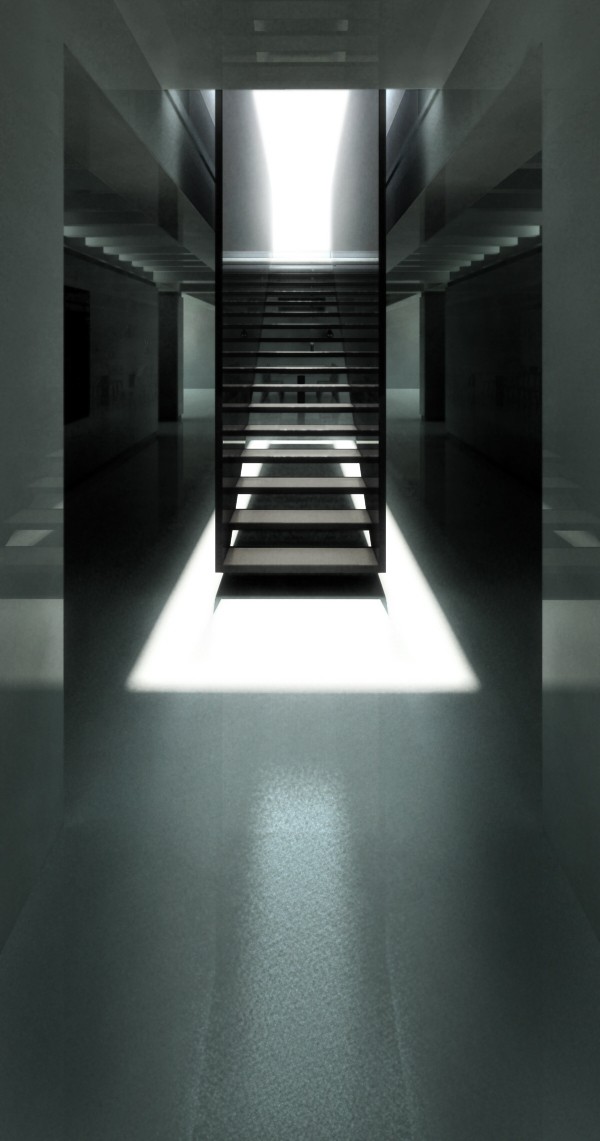
\includegraphics[width=0.4\linewidth]{images/SCP.001.keter.duty.jpg}
    \caption*{SCP-001的内部。}
\end{figure}

\bb{项目编号:}SCP-001

\bb{项目等级:}Thaumiel

\bb{特殊收容措施:}SCP-001的收容措施由监督指挥部制定,并作为单个收容措施统一执行。SCP-001内的各个收容单位皆适用一部分的收容措施。

指派于各收容单位的人员需各自分离,且只能拥有阅览各自收容文件的权限。若有人员阅读其他文件,或试图将SCP-001-K实体曝露于他人,需进行V级记忆删除并调离职位。

\begin{center}

\tred{存取SCP-001图样范例}

\tred{允许存取}

\begin{longtable}{|m{0.3\linewidth}|}
\hline
\multicolumn{1}{|c|}{SCP-001-K}\\
\hline
\endhead
\hline\multicolumn{1}{r}{\small{接下页}}
\endfoot
\hline
\endlastfoot
\raisebox{-.5\height}{
\includegraphics[width=\linewidth]{images/SCP.001.keter.duty.2.png}}
\end{longtable}

\end{center}

各收容隔间的门上都贴有一仪式化的标志,需即时维护。任何污损都会导致收容隔间逐渐消弱,直到收容循环无法持续。由于标志是以石材雕刻而成,维护应着重于预防风化以及外力破坏。

所有SCP-001-K实体都被收容于SCP-001中。只允许拥有六级权限的人员与SCP-001-K实体进行直接互动,而权限低于五级的人员则会授予伪造的收容文件。其他基金会收容的项目也将被归类为Keter以维持该等级的伪装。SCP-001-K实体不可被释放至SCP-001外,除非是在加速VK级现实重组的决议下。

若此一事件发生,六级人员将联系基金会人员以下达后续指令。

\bb{描述:}SCP-001是对所有被归类为Keter等级的异常项目的来源的代称,权限低于五级的人员仅能知悉这些项目的SCP文件。

SCP-001的设施位于{[}删除],高十一层楼并有四座翼楼。外观表现为一高大而无特色的研究设施。尝试详细记录SCP-001的外貌出现了矛盾不一致的报告。尝试绘制设施内部格局则产生相互冲突的楼层布置。目前观察到内部有宿舍、餐厅、娱乐区及办公区。收容隔间仅对五级以上人员开放。

目前已知存在有285个SCP-001-K实体。

SCP-001-K是所有源自SCP-001的异常项目的代称。在发现的当下,所有SCP-001-K实体都被收容于SCP-001中,但迄今已有部分遗失。每个SCP-001-K实体都与另一个能相互抵销异常效应的实体收容在一起。

当任两个SCP-001-K实体之间的收容循环被破坏时,收容隔间将发生局部性的异常现象。收容隔间内的物理法则将会改变,以符合所有未收容的SCP-001-K实体的异常效应,此现象包括但不限于触发此异常的实体。

SCP-001最早由二次大战后驻扎于希腊的美国陆军所记录。当异常性质被发现后,数个组织立刻宣称自己拥有此地的控制权。由于若干SCP-001-K实体遭到释放,迄今仍无法复原这段时期SCP-001的收容资料。

\begin{longtable}{m{0.3\linewidth}m{0.6\linewidth}}
\hline
被指定为SCP-001-K的项目 & \multicolumn{1}{c}{收容方式}\\
\hline
\endhead
\hline\multicolumn{2}{r}{\small{接下页}}
\endfoot
\hline
\endlastfoot
\hyperref[chap:SCP-718]{SCP-718},\hyperref[chap:SCP-689]{SCP-689} & 数个SCP-718被放置于木乃伊化的人体上,以SCP-689为中心围成一三角形。所有实体会不定期地转开视线,导致SCP-689出现在其中一个人体并消灭SCP-718,造成更多SCP-718的产生。此时其他SCP-718会恢复观察,迫使SCP-689回到原本的位置。\\
\hyperref[chap:SCP-990]{SCP-990},\hyperref[chap:SCP-122]{SCP-122} & 数个SCP-122实体被观察到以身体阻挡外界的声音与光线,并在SCP-990的身边念床边故事,以确保后者在物理世界中持续沉睡。\\
\hyperref[chap:SCP-1178]{SCP-1178},\hyperref[chap:SCP-1984]{SCP-1984} & SCP-1178悬浮在立方体房间中,SCP-1984紧追在后。目前已知有六种不同的追赶方式作随机更换,SCP-1984被观察到距离SCP-1178至少15公尺远,只要SCP-1984加速,SCP-1178也跟着加速。收容人员目前正研究如何减轻SCP-1178被SCP-1984引爆时产生的伤害,并防止它摧毁其他SCP-001的收容设施。\\
\hyperref[chap:SCP-1440]{SCP-1440},\hyperref[chap:SCP-836]{SCP-836} & SCP-1440被铐在一宽敞圆形房间的门上,周围的建筑结构被SCP-836影响而不断朝SCP-1440靠近,并被项目的异常性质摧毁。SCP-1440表示他被一位神父所囚禁,除此之外没有其他相关资讯。\\
\hyperref[chap:SCP-1048]{SCP-1048},\hyperref[chap:SCP-1055]{SCP-1055} & SCP-1048持续地剥下SCP-1055新生的物质来建构新的实体。SCP-1055不断移动,并摧毁靠近的SCP-1048。这些残骸又会被制造成新的SCP-1048或用来修补其他实体。目前隔间内估计有████只SCP-1048,而隔间的容量估计是██████████只。\\
\hyperref[chap:SCP-1295]{SCP-1295},\hyperref[chap:SCP-871]{SCP-871} & 一个服务生装束的金发女性人类\footnote{似乎是SCP-001的一部分}不断为四个SCP-1295实体送上SCP-871,她从一张木桌上持续拿取SCP-871并端给SCP-1295。四个实体都在抱怨菜单单调,但称赞SCP-871的品质与种类。\\
\hyperref[chap:SCP-505]{SCP-505},\hyperref[chap:SCP-140]{SCP-140} & SCP-505被悬挂在SCP-140上方,以70,000字\slash 15分的速率写下关于Daevite文明与文化的信息\footnote{以希腊字母写成。}。由于SCP-505叙写的文字已经超过目前的时间达七十年,中断此循环可能会导致人类历史全面而不可逆的改写。\\
\hyperref[chap:SCP-231]{SCP-231},██:██-N & {[}删除]和一已遭消灭的异常项目的剩余互动。收容迄今,除了六次潜在的失效以外,110-蒙托克程序已成功预防这种互动所产生的XK级事件。为了阻止VK级事件而采取的蓄意失效已提交监督指挥部审理中。\\
\hyperref[chap:SCP-058]{SCP-058},\hyperref[chap:SCP-1983]{SCP-1983} & SCP-058被悬挂在一圆洞上方,洞中放满了仍在跳动的人类心脏。SCP-058的内部和周围塞满额外的心脏组织。SCP-1983实体不断从房间昏暗处试图将组织从SCP-058身上扯下,SCP-058一面击退它们,一面从洞中同化更多心脏组织。\\
\hyperref[chap:SCP-682]{SCP-682},\hyperref[chap:SCP-296]{SCP-296} & SCP-296内的实体皆为人形,特征符合在维持项目收容时死亡的人员。SCP-682无法伤害这些人形,时而狂暴地试图杀死它们,时而畏缩在收容隔间的中心。当Dr. ██████ █████████问起时,SCP-296表示SCP-682获判有罪,因此处罚其不得杀人或自杀。\\
\hyperref[chap:SCP-579]{SCP-579},\hyperref[chap:SCP-055]{SCP-055} & 圆榫打不进方洞。
\end{longtable}

\bb{附录001-A:}

\tred{需要六级权限}

\tred{允许存取。欢迎,监督者。}

\begin{scpbox}

找回来了么?

我们能看到彼岸,人事已非,但我们也在进步。

提案是最新的紧急命令,所有K级项目的研究立刻中止,并以收容而非传播的原则重新进行。灾难已经带走太多人命了,该让事情回到

\{\{

清洗行动已经大幅扩大,Olympia中的项目皆已完全收容,感谢红色使我们能够长期预防任何事件发生。在你之中可以找到更多关于收容策略的信息。笑一个吧。

事情正逐步改善。我们已经让色彩重新运作,我听说他们不久之后也会把人们的知觉取回。如果你看到第七新娘,请表达我对于她打开盒子一事的遗憾,或许她会记得。

\end{scpbox}

\bb{附录001-B:}VK级现实重组是当所有SCP-001-K实体皆从收容循环中被释放时,理论上会出现的异常现象的代称。如果所有SCP-001-K实体都被释放了,这个效应将改变已知的宇宙,使其在一无异常的物理法则下运作。目前正在研究基金会如何适应这种变化以及如何保护新宇宙和当下的现实。


\chapter[SCP-001 孩子们]{
	SCP-001 djkaktus - The Children \\
	SCP-001 孩子们
}

\label{chap:SCP-001.the.children}

\newcommand{\vdotsc}[1]{\cl{\multido{}{#1}{. \\}}}

\begin{scpboxbbwmc}
\GG{\wred{\bb{警告:以下文件被分类为}}}

\Hg{\wred{\bb{5级}}}

\GG{\wred{\bb{此分类由监督者议会授权}}}

\g{\bb{任何未经5级授权试图访问该文件的行为将被记录,并且查阅者将被处决。}}
\end{scpboxbbwmc}

\hr

\vdotsc{7}

\begin{scpboxc}
输入五级基本安保证书
\end{scpboxc}

\vdotsc{7}

\begin{scpboxc}
Command:\textbackslash users\textbackslash O513>\_ 6110298-父罪与子罪-3561840
\end{scpboxc}

\vdotsc{7}

\begin{scpboxc}
允许访问,初级模因抹杀剂解除,晚上好,O5-13。
\end{scpboxc}

\vdotsc{7}

\begin{scpboxc}
警告:此文档部分内容已被锁定。
\end{scpboxc}

\begin{scpboxc}
解锁需要额外的5级权限。
\end{scpboxc}

\vdotsc{7}

\hrule

\begin{figure}[H]
	\centering
	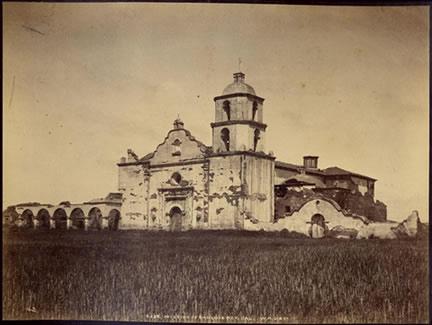
\includegraphics[width=0.5\linewidth]{images/SCP.001.the.children.jpg}
	\caption*{位于墨西哥圣马可的San Marcos de la Vida Eterna教堂,\\ 照片上的日期为07/27/1903}
\end{figure}

\bb{项目指定编号:}Item-001

\bb{收容等级:}Keter-Thaumiel

\bb{收容状态:}激活-稳定

\bb{收容措施:} 物体-001(Item-001)现在正被收容于墨西哥的圣马可,收容地点位于San Marcos de la Vida Eterna教堂的旧址地下。原始收容措施已经证明可以有效收容物体-001。收容区域现在被指定为一个高安保级别的军队废物处理厂,墨西哥法律则禁止所有平民接近该站点10km范围内。围绕物体-001的收容区域将有自动化闭路监控无人机进行巡逻,并且这些无人机被设计为一旦见人将格杀勿论。

\bb{O5备忘录001-Alpha:}\ii{对于有关SCP-001,也就是前物体-001,的所有信息收容将成为最高优先事项。我已经授权将资料库之中相关资料清除,并在原地址上创建数个错误项目。如果真的有人能追查到那个地址,那些伪装项目也足够让他们感到失望了。我现在抽出了好几个EX的SCP项目放置在那个地址上,直到我们找到更好的伪装项目为止。}

\ii{删除你找到的任何信息,堵住任何可能的漏洞,将这些信息掩埋在你觉得足够多的模因抹杀剂之下。要做到这一点,你需要做比完全删除资料还要多的多的工作。-O5-2}

\bb{项目描述:}物体-001是对9名人类组成的群体的指称,这些人年龄在4-11岁不等.他们因为001项目:“神之双子”(Twins of God)(见项目提案001以获得更多信息)而取得了异常性质。因为对物体-001进行了不当使用,导致了一名高级人员的死亡,这也使得对其进行处决变得必要。作为这一事件的结果,物体-001现在按照现有收容措施进行了收容。所有9名物体-001的个体都在功能上已经进入了脑死亡状态,但却仍然表现出生命体征,而不论对其的收容措施情况如何。

物体-001的个体都放射出大量的伽马射线,放射量通常都在███GJ以上,并且以一种独特的形式进行变换。当每个个体单独收容时,这种放射模式似乎是随机的,但如果将这些个体进行集合收容时,这些放射模式似乎会出现某种确定的特征。因此,每一个个体之间收容间隔大约应保持在████。另外值得注意的是,物体-001的个体是具有辐射发光性的。在这些个体进入激活状态时,对它们进行视频监控是不可能的,因为在此状态下的个体出现在屏幕中时将导致录影脚本发生损坏。

当一个物体-001个体与其他个体之间相隔小于20m时,它将表现出对物体、人类个体或是某块区域的远距离毁灭能力。对于此性质将会稍后在此文档之中进行详细描述。

根据监督者议会的命令,物体-001被分类为一个Thaumiel\footnote{"Humphrey, W., Lemke, R., Christian, K., Roesler, J., \& Kaiser, N,(1920),《收容分级提案:Thaumiel》,基金会研究出版社,2(7)。"}-Keter实体。

\vs\hrule

\begin{scpboxbbwm}
\bb{警告:}有关物体-001的更多信息已经锁定,并且已经被分类为5级。模因抹杀剂已经插入其中保证有关于物体-001的信息不会出现外泄。非监督者议会成员,并且不具备5级模因抵抗条件的人员将会受到模因抹杀剂影响而被处决。\bb{\ii{你已受到警告,并且这是最终警告。}}
\end{scpboxbbwm}

\cl{\bb{项目提案001: 锁定}}

\cl{\tred{+ 输入授权密码}}

\cl{\tred{1485992-13人乘死者船-4910581}}

\begin{scpboxc}
{[模因抹杀剂无效化]}
\end{scpboxc}

\begin{scpboxbbwm}
\GG{\bb{\tred{项目提案:“神之双子”}}}

\Gg{研究团队:Omega-5}

\g{\bb{项目日期:02/13/1922}}

\Gg{\bb{目的阐述:}}

\ii{此项目旨在创造出一个异常实体,该实体能在基金会中心高层必要的掌控之下,对基金会及全球安全造成威胁的敌意异常个体加以远距离摧毁。}


\bb{研究团队主任:}Dr. ███ █████,Ph.D.(O5-1)

\bb{副主任:}████ ██████ (O5-2),████ ████(O5-3)

\Gg{\bb{项目需求:}}

\begin{itemize}
	\item 取得并且使用物体-███:“亚原子加速系统”。
	\item 取得并且使用物体-███:“Harken之门”。
	\item 取得并且使用物体-███:“多重注射器”。
	\item 能够制造必要收容措施和研究设施的材料。
	\item 不少于50名成年人类个体(D级)作为测试目的之用。
\end{itemize}
	
\Gg{\bb{项目细节:}}

通过分析最近从物体-███和物体-███实验之中取得的信息,一个之前不可能出现的机会摆在了基金会面前:一种能力,能够穿越远距离改变物体量子组成,从而导致该物体从功能上不复存在\footnote{Maxwell, T., \& Gouram, A.(1927),《远距离上的量子性质》,基金会研究出版社,05(02),213-230页。}的能力。到目前为止,通过使用物体-███来改变人体性质从而对这一效应加以更大的操控,我们认为这一点是可以做到的。为了达到我们的最终目的,物体-███、物体-███和物体-███已经从基金会记录之中抹消了,并且它们将会单独收容在这个项目最初的研究设施之中。

在美国核试验设施的幌子之下,我们将在墨西哥北部建立一个站点,远离人群,这也是出于对这一理论进行安全测试的考虑。为了将这些实验对自然性质可能造成的潜在影响降到最小,我们将对这一项目进行最高的防护措施,对灾难性收容失效事件也建立了数个意外保险措施。这些保险措施将会在下面列出。

如果这一项目最终成功,这些实验创造的实体,暂时指定为物体-001的控制权,将交由基金会管理者掌控来对抗我们指定为GOI-003“地狱王国”(Kingdom of Abbadon)的异常敌对组织,一系列心灵抹杀剂将植入这些实体之中,对于这些抹杀剂的取得也只对管理者单独开放,这是作为确保这些个体不会落入敌对组织控制之中的保险措施。

\end{scpboxbbwm}

\begin{scpboxc}
{[模因抹杀剂无效化]}
\end{scpboxc}

\begin{scpboxbbwm}

\GG{\bb{意外保险收容措施:}}

\bb{Alpha:} 当出现灾难性收容失效事件时,植入这些实体之中的心理抹杀剂将启动,将其处决。每一种抹杀剂都被赋予不同的优先级并且应按顺序使用,以下是优先性列表:

\begin{itemize}
	\item Berkeley剂:降低身体活动能力。
	\item Anastasia剂:降低异常性质[正在开发中]。
	\item Nezbit剂:降低心理能力。
	\item Orion剂:对高级神经系统的全面化学性溶解。
\end{itemize}

\bb{Beta:} 在Alpha保险措施失效的情况下,安保人员应前去处决物体-001。将这些个体捕获的可能性不大,也不推荐这么做。建议相关人员与物体-001个体之间保持安全作业距离,并且穿着必要的基金会开发的反辐射防护装甲。同时推荐进行远距离弹道射击,因为这一行动将不会那么快吸引物体-001个体的注意。

\bb{Delta:}在Beta保险措施失效的情况下,基金会控制的长距离弹道武器将启动并且直接作用于物体-001个体上。我们将在研究设施外建立一个10km的边界,不少于10架重装轰击加农炮部署于这一边界上。在Delta措施启动时,它们将用于处决物体-001。

\bb{Epsilon:}在Delta保险措施失效的情况下,站点自身装载的自爆装置将启动,基金会管理者将全程监督Epsilon措施的实施情况。

\Gg{\bb{项目批准:}}

\begin{figure}[H]
	\captionsetup{singlelinecheck=false}
	
\includegraphics[max width=\linewidth]{images/SCP.001.the.children.2.png}
	\caption*{\ii{基金会管理者R. D. Fritzwilliams}}
\end{figure}

\begin{figure}[H]
	\captionsetup{singlelinecheck=false}
	
\includegraphics[max width=\linewidth]{images/SCP.001.the.children.3.png}
	\caption*{\ii{项目主任O5-1}}
\end{figure}

\end{scpboxbbwm}

\cl{\bb{项目报告001-Delta: 锁定}}

\cl{\tred{+ 输入授权密码}}

\cl{\tred{- 7483529-九分钟后午夜-1889475}}

\begin{scpboxc}
{[模因抹杀剂无效化]}
\end{scpboxc}

\begin{scpboxbbwm}

\GG{\bb{\tred{项目“神之双子”进程报告}}}

\Gg{研究团队:Omega-5}

\g{\bb{项目日期:04/18/1924}}

\bb{进展细节:}

对于新物体-001个体的收容立刻就出现了问题,因为在约35\%活跃项目人员之中产生的[从记录之中删除]和急性放射病,我们出现了█人伤亡。对于收容措施的调整变得很有必要,以及这个现在我们指定为站点-001的站点内部结构也进行了强化。人员的住所已经后撤到了一处里主要研究设施有5km远的地方。

在苏丹,一次由地狱王国主导的对基金会设施袭击再次加剧了对远距离防卫系统的紧急需求,也同时加快了激活物体-001的时间表。在基金会管理者的命令下,我们得到了额外的物资来发展更为高效的实验设施。

另一件核心要件则是如何将异常性质收容在一个人类个体之中。在所有100\%的实验个体之中,尽管异常性质都只出现了一些小事故就能收容在他们体内,但所有的实验个体都会立刻瘫痪并且出现严重的脑溢血。而异常性质发挥效用的唯一证据则是站点结构或人员的随机突发毁灭,理论认为这一现象是因实验个体心理控制力恶化,无从控制这些异常性质而导致的。在所有100\%这些情况下,我们都启动了心理抹杀剂来将这些前物体-001个体处决。

站点外人员主导的另一项实验给了我们灵感,或许将这种异常性质平均分散到数个人类个体体内是可能的\footnote{Enjilian, M., \& Johnson, R.(1923)《数个Keter项目的异常性质》,基金会研究出版社,1(11)。},如此一来异常性质对人类个体心灵造成的压力问题将得以解决\footnote{Everly, K., \& Everly, J.(1922)《被消灭的Keter实体的大脑结构:对超自然个体认知结构的进一步分析》(第三版,第一章,自费出版,145-178页)芝加哥,IL:基金会科学出版社。}。

在一次使001号站点运转能力降低的测试,以及在基金会管理者命令下将D级人员转出站点到其他课题的行动之后,我们不得不讨论项目是否能继续进行这一问题。在与17号站点的主任进行咨询之后,一队武装特工进驻了墨西哥圣马可的San Marcos de la Vida Eterna教堂,并且他们还找来了一群年轻人进行测试。我们对圣马可城全体市民都进行了A级记忆消除,而这些人则之后被转送到了09号站点以备下一步之用。圣马可城本身则成为了新的001测试站点,23名最健康的个体被挑选出来进行实验,而剩余个体则全数处决。

\end{scpboxbbwm}

\begin{scpboxc}
{[模因抹杀剂无效化]}
\end{scpboxc}

\begin{scpboxbbwm}

\Gg{现状:}

现在这个项目准备进入下一阶段,下一阶段的实验将会在新的001测试体上进行,这一实验还在等待来自中央控制层的命令。以下这封信是申请将项目推进到下一阶段的,内容如下:

\begin{scpbox}

04/03/1924\\
致:基金会管理者\\
自:Omega-5团队负责人

管理者Fritzwilliams:

正因为从您办公室之中发出的每一条缩减预算和削减补给的命令,我们的项目随着每一条这种命令的发出而越来越难以保持进度。在中央控制层还没有主动与我们进行联系的情况下,我们只能认为对我们的指示是不变的。

一份为帮助我们项目尽快获得结果而寻求物资帮助的申请很快也会到达您那里,我们希望您能看到形势的变化,并且给我们的一个良好的答复。如能及时回信,不胜感谢。

███ █████\\
项目负责人

\end{scpbox}

04/15/1924\\
致:Omega-5团队负责人\\
自:基金会管理者

█████:

我们给你下达的指令依然没有改变。如果你们的项目能够成功,那么我们就大可高枕无忧了。但很不幸的是,严酷的事实时刻提醒着我们,我们身陷一场战争之中,而物资又是如此贫乏。为了保证我们事业的隐秘性,我们再没有面对过比这状况更严峻的时期了,更不要谈继续你们的研究。但我仍会尽我一切努力帮助你们,不为别的,只因为你们的研究能从地狱王国手中保护我们。

我已经接到了你们的申请,尽管从道德上我没有任何理由去批准它,但我作为基金会领导者还是强迫自己批准了它。市民随便你们挑,但只允许挑成年人,也不要肆意践踏无辜者的生命。上帝知道,为了我们的目的已经有足够多的无辜者鲜血洒下了,我不希望再看到更多。

管理者Fritzwilliams\\
基金会中央管理层

\end{scpboxbbwm}

\cl{\bb{文档:GOI-3“地狱王国”: 锁定}}

\cl{\tred{+ 输入授权密码}}

\cl{\tred{- 4561273-影覆沙丘-0948390}}

\begin{scpboxbbwm}

\GG{\bb{\tred{同行组织文档003}}}

\Gg{\bb{指称:地狱王国(Kingdom of Abbadon)}}

\bb{威胁等级:}非常高\\
\bb{活跃等级:}非常高\\
\bb{优先度:}5级

\bb{综述:}GOI-003“地狱王国”是对一群异常敌对人性个体的指称,他们现在位于撒哈拉沙漠的某处,该处根据其手稿之中的描述被称为“吾等神王Abbadon之城”。这些人形个体从很多方面都与人类相似,但他们所有成员都至少是I级现实扭曲个体。\footnote{Benson, R.(1921)《现实扭曲个体分级》,基金会研究出版社,3(7),10-58页。},同时高级个体已经达到了III级或者IV级的现实扭曲分类。由于他们本身异常性质之强烈,对它们的捕获和收容是不可能的,并且任何这方面的尝试都十分危险。

\bb{最初发现:}GOI-003最初是由法国军队人员于1912年,对一起利比亚北部村落的袭击行为调查之中发现的。军队的护卫队遭到了袭击,80\%的人员死亡。幸存者称他们被不多于6个人的“巫师们”袭击了,这些“巫师”能进行飞行,并且可以抵挡枪械攻击。这些幸存者,以及可能的目击者都被给予了记忆消除之后释放了。

基金会人员最早遭遇GOI-003人员是在一次对埃及南部破碎之神教会仓库的袭击尝试之中,就在那次行动之中,机动特遣队Alpha-4“无疆”(No Borders)被一群与法国军人描述一致的异常个体袭击。机动特遣队Alpha-4成功击退了它们,并捕获了一名低级成员。在对这名俘虏进行处理和审讯之后,基金会知晓了“地狱王国”的本质,中央管理层开始采取措施保证基金会不受到这个异常组织的侵扰。

根据收集到的数据,“地狱王国”原本只是一个阿拉伯半岛现实扭曲者组成的团体,希望在撒哈拉的不毛之地之中开辟属于他们自己的国家。由于他们本身所具有的异常性质,他们可以将严酷的地形变为他们所需要的,同时利用这种地形确保侵入者远离他们的国家。随着时间的推移,他们的数量随之增加,新生儿将被带到国家的统治者“Abbadon神王”面前转变为现实扭曲者。

但是,由于成员之间的近亲婚育和基因障碍对他们社会产生的毒害,地狱王国本身变得十分脆弱,并且在20年内就难以作为一个独立的组织存在。收集的数据显示地狱王国自身已经知晓了这一点,并开始展开行动防止这一未来的发生。到目前为止,基金会部署在非洲大陆内部及其周边的许多设施都已经遭到了该组织激进成员的攻击,基金会为此付出了不少于75条人命的代价,并且至少有12件异常物体被偷走。

\bb{结论:}因为对抗地狱王国成员这一行为本身的难度和危险性,同时也因为对他们的行为缺乏情报,不建议任何人员在缺乏重型武器部队时与地狱王国成员发生冲突。对抗地狱王国手段的研究现阶段正在进行中。

\end{scpboxbbwm}

\cl{\bb{备忘录001-Alpha:锁定}}

\cl{\tred{+ 输入授权密码}}

\cl{\tred{- 7105922-无情神明之眼-0981478}}

\begin{scpbox}

\bb{日期:}11/29/24\\
\bb{用户:}Omega-5-1\\
\bb{主题:}001

就这样,我们做到了。我们做到了不可能的事情。我们狠狠打了神一耳光并且把他的冠冕抢到了我们手上。

这是一个新的充满荣耀的日子。

5有关于将异常性质平分到一个集体之中的看法是对的。在之前的实验体之中,尽管我们已经尽我们所能加固他们的身体,但注入他们身体的总计███的能量还是太多了。我没法告诉你那些D级人员的数量,那些我们只能看着他们的皮肤从他们的骨头上融化,他们的骨头碳化之后如同尘土飞散,最后我们不得不把他们从地上铲走的D级人员。几十名?几百名?我不知道。比我们期望的多得多,也比基金会可以容忍的要多的多,即便是我们这样的项目之中。

13对我们在墨西哥所做的一切表示遗憾,但13是短视的,管理者也是短视的,一些人的死亡,甚至是许多人的死亡,与防止世界被毁灭较之如何?一文不值。那些孩子们现在已经是神了,他们的生命是为了一个更崇高的目的而存在的。还有什么生命,能比得上全知全能呢?

明天即将开始实验,你听得到吗?

\end{scpbox}

\cl{\bb{项目报告001-Delta: 锁定}}

\cl{\tred{+ 输入授权密码}}

\cl{\tred{- 7483529-九分钟后午夜-1889475}}

\begin{scpboxc}
{[模因抹杀剂无效化]}
\end{scpboxc}

\begin{scpboxbbwm}

\GG{\bb{\tred{项目“神之双子”进程报告}}}

\Gg{研究团队:Omega-5}

\g{\bb{项目日期:01/17/26}}

\bb{进程报告:}

现在,9名被集合指定为物体-001的个体已经被收容于一个进行过加固的仓库之中,并且在测试站点01进行试验。这些个体在执行指令而启动时,没有表现出高级脑部活动的迹象。尽管如此,这些个体整体能够对信息进行处理,并且能以在对其进行的每个个体模因循环控制的过程中加入信息的方法加以控制。

所有这些个体现在都是V级辐射活跃危害元,人员禁止在没有穿着抗辐射装甲的情况下进入物体-001周边1km以内。每个个体之间放射伽马射线的模式是随机的,但当他们聚集到一起的时候,他们的辐射模式变得类似于一名清醒人类在脑电波扫描器(EEG)上表现出来的脑波模式。但尽管有所相像,比起正常人类的脑波模式,这种模式更具有随机性和不一致性。

物体-001整体能够共同引导一种来自于我们未知的地外空间的庞大能量,并且能够运用这一能量在量子层面上将分子分解。这一性质使得它们可以在任何距离上将任何物体不为人知地加以歼灭,只要这一物体的特征和所在地点对物体-001进行了一定程度上的详细描述。

以下是物体-001于01/17/26的测试结果:

\hr

\bb{测试序列023}\\
\bb{对象:}物体-001\\
\bb{研究团队:}Omega-5

测试目标:确定物体-001效应的最远边界

\bb{第1轮:}测试物(钢条)放置于物体-001 5km远处。物体-001被操作者(███ █████博士,Omega-5负责人)下令摧毁目标物体。

\bb{结果:}测试物体在物体-001收到指令并且执行之后不久被消灭。与测试之前相比,目标物没有任何质量留存。

\bb{第5轮:}测试物(钢条)放置于物体-001 800km远处。物体-001被操作者(███ █████博士,Omega-5负责人)下令摧毁目标物。

\bb{结果:}测试物体在物体-001收到指令并且执行之后不久被确认消灭,距离对于这一效应而言没有影响,更远距离的测试将加入下一序列的实验之中。

\ii{这些孩子如设计好的一般对命令加以了执行,我对他们在时机成熟之时成功执行使命毫无怀疑。他们毫无动摇,毫无感情,同样也不可摧毁,在跨越宇宙将死亡降临之前也仅仅只需要一个命令而已。诚然,这就是为人类之中最刚毅者设计的武器。 - O5-1}

\hr

\bb{测试序列025}\\
\bb{对象:}物体-001\\
\bb{研究团队:}Omega-5

\bb{测试目标:}确定远距离摧毁时物体大小的上限以及下限

\bb{第2轮:}测试目标(铁球,直径3m)放置在距离物体-001 1000km的位置,物体-001被操作者(███ █████博士,Omega-5负责人)下令摧毁目标物。

\bb{结果:}测试物被消灭,如同预想一般

\bb{第3轮:}测试目标(破碎之神教会的工坊,位于土耳其的███████████)距离物体-001 11500km,物体-001被操作者(███ █████博士,Omega-5负责人)下令摧毁目标物。

结果:目标被消灭,在其周边区域没有发现额外的损伤。这一事件的目击者被给予了A级记忆消除并且释放拘捕以进行额外的实验。测试显示这些个体,或者这一个群体需要精确指定目标,仅仅指定某一个地区不足以让它们进行消灭。

\bb{第7轮:}测试目标(成年男性,33岁)距离物体-001 11500km,物体-001被操作者(███ █████博士,Omega-5负责人)下令摧毁目标物。

结果:目标被消灭

\end{scpboxbbwm}

\cl{\bb{收集的相关基金会通讯及通知: 锁定}}

\cl{\tred{+ 输入授权密码}}

\cl{\tred{- 0002481-警惕之眼-4781621}}

\begin{scpboxc}
{[模因抹杀剂无效化]}
\end{scpboxc}

\begin{scpbox}

\bb{日期:}02/01/26\\
\bb{致:}Omega-5团队负责人\\
\bb{自:}管理者Fritzwilliams

我已经知悉你们在001项目上大获成功的好消息,我完全无法描述这一成功是多么重要。我们终于可以将地狱王国画上一个句号了,并且在未来,我们将能更好地保护自己。在这一刻,我对你们的工作致以永恒的感激。

但,我必须明确提出对你的忧虑,O5-1。尽管你取得了重大成功,但最近你的来信让我烦心。我对你是Omega队的最佳领袖这一点毫无怀疑,但我还是觉得这一成就的压力是否在你的身上造成了某种代价。我知道自己已经为此付出了代价。不论如何,只要这一切结束,我准备将你提拔成为新建的19号站点的主任,当然,这会是在你进行足够的休息重新恢复过来之后的事情了。在下个月我和你的会面时刻我们可以详谈此时,到时候我们已经把地狱王国的一切都安排妥当了。

你真诚的

管理者Fritzwilliams

\end{scpbox}

\begin{scpboxc}
{[模因抹杀剂无效化]}
\end{scpboxc}

\bb{日期:}02/14/26\\
\bb{致:}基金会中央管理层\\
\bb{自:}Omega-5团队负责人\\

我很好,管理者。这个项目已经完成了,你到来的时候我们就能完成我们的使命了。

\ii{1}

\begin{scpboxc}
{[模因抹杀剂无效化]}
\end{scpboxc}

\begin{scpboxbbwm}

\Gg{全员通告:全人员}

\Gg{[由监察者命令编辑]}

\Gg{\bb{由基金会中央管理层发布}}

\bb{日期:} 03/21/26\\
\bb{主题:}管理者Frizwilliams

基金会管理者R. D. Fritzwilliams已经遭到谋杀。我们已经发布了一份全基金会通缉令以缉捕杀害他的凶手及其帮凶:███ █████博士、████████ ████博士、████ ██████博士、█████ ██████博士以及██ ████特工。我们认为这些人员持有武器并且十分危险,并可能持有一个高危异常物体。如果你手上有任何有关于这些人员所在地信息,请直接向站点主任报告。

我们已经成立了一个临时管理议会,主要成员由Omega-5团队的高级指挥人员组成,这一人事任命是由已故的管理者下达的。这一议会将会持续监督基金会行动,直到我们能选出一名新的管理者为止。

\end{scpboxbbwm}

\begin{scpboxc}
{[模因抹杀剂无效化]}
\end{scpboxc}

\begin{scpboxbbwm}

\Gg{全员通告:全人员}

\Gg{\bb{由基金会中央管理层发布}}

\bb{日期:} 03/22/26\\
\bb{主题:}对GOI-003调查队的解散

\bb{通知:}\ii{我们认为以下机动特遣队调查队已经处于无行动状态,这些机动特遣队人员应向17号站点主任进行报告:}

\ii{机动特遣队Alpha-1:“王的侍从”(All The King's Men)}

\ii{机动特遣队Alpha-2:“地球之盐”(Salt of the Earth)}

\ii{机动特遣队Alpha-3:“哈佛男孩”(Havard boys)}

\ii{机动特遣队Alpha-4:“无疆”(No Borders)}

\ii{机动特遣队Alpha-5:“兄弟羁绊”(Band of Brothers)}

\ii{机动特遣队Alpha-6:“黑暗证言”(Dark Testimony)}

\end{scpboxbbwm}

\begin{scpboxc}
{[模因抹杀剂无效化]}
\end{scpboxc}

\begin{scpbox}

\bb{日期:}11/01/26\\
\bb{致:}监督者议会\\
\bb{自:}23号站点主任Harrison\\
\bb{主题:}23号站点勘探报告

我的手下带着报告回来了。我将现场照片随信附上,但我还是无法相信着一切。什么都没有了,只有永恒不变的沙漠。就像他们从没有出现在那里过一样。

我让他们仔细检查,你们是对的,没有留下任何尸体。不过本来那里也就该什么都没有,不是吗?

不论如何,我不知道你们被迫和魔鬼做了怎样的交易,但谢谢你们。

\ii{-Harrison}

\end{scpbox}

\hr

\vdotsc{14}

\begin{scpboxc}
你已经三分钟没有操作这个终端了,你需要帮助吗?
\end{scpboxc}

\vdotsc{14}

\hrule

\bb{新语音文件:}

\tred{► 开始录音}

\tred{❚❚ 暂停录音}

[开始录音]

我觉得这是该干这事情的时候了,趁我还能记得一切的时候早早干了比较好。距离我读这篇文档已经过去很长时间了,这时间长得可以追溯到'26年的那个晚上。距离人们可能知道我们所作所为的真相,到底在地狱王国、O5-1和管理者身上发生了什么事情已经过去太长的时间。该死。如果这一切都已经掩盖在记忆消除之下,那么我可能是最后剩下的一个了。

我绝不会把这一切带进坟墓里的,至少这一件事绝对不会。

一总是有着超凡魅力,这一点在各种记录上已经描述得够多了。这就是为什么Fritzwilliams给了他Omega-5团队管理者的身份,把他置于二之上,即便二在基金会里待的时间比一要长得多。这并不是说一并不聪明,恰恰相反,他是我一起共事过的最杰出的研究者之一,就算过了这么久也是如此。他写作了所有Omega-5团队研究的报告,在我们离一个成熟的队伍还远着的时候他就已经这么做了。在当时我们只是17号站点初级研究员之中的一小群而已,而他,雄辩、热情而又\ii{偏执}。

他又是那么超然。他爱着他的事业,请不要误解我,研究对于他而言是最高的愿望。但对于基金会的指示,或者是有关收容带来的压力,他一点兴趣都没有。他多次对我说,我们没有充分利用资源。如果我们不是那么害怕这些异常物品,我们本可以对他们进行更好的收容的,但我们就是害怕用一些异常物品去收容另一些的方式。当然,也是他,是Thaumiel级别的最初分类设计者,他和Epsilon-2队伍完成了这一编级。我想,这或许是他为何对抓住机会参与到我们在001项目之中的工作之中如此热忱的原因。

001项目,那是如此地超凡脱俗,前所未见,但同时,地狱王国也是如此。记录在这里的文档连它特别之处的一半都无法描述,而其他的部分都已经散佚在历史之中。在地狱王国面前,我们与之相较简直就是疯狂而滑稽。一群得到了庞大资金支援的科学家和武装部队,对阵一小群绿型个体(type-green)的军队,我们甚至都不知道他们的弱点在哪里。II级和III级能做到的事情,已经远超出我们所能办到的,这事情还发生在我们见到第一个斯卡兰顿现实稳定锚半个世纪之前。一些报告称他们的统治者是个V级。如果那是真的,只要他想,眨眨眼睛就能把我们从地图上抹掉。

在1922年整一年之中,地狱王国一个组织要单独为所有基金会站点的摧毁事件负责。当然,这些事件不仅仅发生在撒哈拉沙漠周边的非洲地带,只是我们从没有公开过而已。地狱王国的活动范围北至直布罗陀,南至马达加斯加。他们暴力闯入站点,毁掉一切,只带着一些物品离开,当然也不忘删掉所有记录。那我们当时在干什么?我们才刚刚开始分类现实扭曲者,更不要说如何和他们战斗了。如果地狱王国对欧洲或者中东的一个更大的站点发起这样的袭击,那就是一场赤裸裸的屠杀了。

如果你在读这个文档,那么你肯定已经看过001的文档了。你知道那是用来做什么的,也知道那是如何做出来的。“为终结所有枪而存在的枪”,从人类身体之中雕刻而出的武器,一旦开火目标可以将任何时间任何地点的任何物体完全湮灭,所有这些只需要一段简短描述而已。一被这些完全吸引住了,被他们,那些孩子们……我到现在还能听到他们的惨叫,听到我们把他们放到机器里,将他们的灵魂抽取出去,再用其他……其他某种东西代替时他们的惨叫声。但这一切都起效了,一对此是如此地自豪。

然后就到了完成我们使命的时刻。管理者从17号站点飞来,那次是我寥寥数次看到他出现在公众面前的机会之一。这样的一次事件就像我们期待的那样,空气之中溢满了严肃,我们都知道肩上的担子有多重,了解到我们正在同时给数百人下死刑判决。我想着,如果当时我们曾经想过我们还有其他选择,可能我们都不会走到那个悬崖边缘上,但……

在我们的注视之下,一走到那些发光的孩子之前,说出了启动口令。他们是……如此辉煌,在某种程度上。人类形态与原始能量的完美平衡体。一将身子前倾,说出了地狱王国城堡的名字,之后他们放射出了剧烈的光芒,一切就结束了。我们没办法知道这一切是起效了还是没有,这一次不同于我们其他的实验可以检验结果。但即便如此,我们还是觉得结束了,就像那种感觉,一口深深屏住的气终于得以释放一样。

然后Fritzwilliams就这么消失了,他的衣服和防护装甲就这样落到地上堆成一堆。就当枪声响起实验室被烟雾堆满时,我们看到1迅速冲向了一个紧急出口,而001又开始发光了。在这之后,一切都乱了套,当机动特遣队冲向实验室收容001时我们静静地向我们的住所走去,一次向其他司令官的快速报告,询问,搜寻,一切都混杂在了一起。

一逃掉了,当然是这样的,他们没有找到他,直到现在也找不到。他不是唯一一个逃走的人,我们队伍之中还有四个人和他一起走了。一部分初级人员,还有15号站点的一半高级人员叛变了。他们都消失得无影无踪,物品也是一样,就在他们的房间外面。调查人员之后发现这一切策划已久,一参与抚养001就是为了这个结局。

我们把这些孩子深深埋藏在圣马可之下,把他们用50m厚的混凝土覆盖起来。在我们把它们放进铅包里时,它们什么都没有说,如果不这样做就什么效果都没有。在我们把它们一一分隔开来的时候,它们也什么都没有说,当我们把它们的坟墓最终合拢时,它们也什么都没有说。我很怀疑它们是不是再也什么都不说了。但我绝不怀疑它们还是活着的。世界上最强大的武器,装弹了,也上膛了,但没有扳机。一就是那个扳机,也只有他是。但愿,这一武器能随着他的消失而从此沉默。

最后,我们就是剩下的管理者,就是我们之中剩下的8个。我们又找了5个最聪明的家伙,于是就把一切强行推进了。地狱王国就此消失,什么都没有留下。除此之外还有烂摊子要收拾,但我们还是找到了把一切继续下去的方法,我们逼着自己去做,到最后,我们克服了一切。

我还在想着圣马可下面的那些孩子,一遍又一遍地想着。想着那些我们在恐惧和恐慌之中走过的时光,想着那些我们做的事情,就算现在脱离了那个项目也是一样。我也在想着一。我好奇他是否找到了他一直追寻的,我也很好奇他是否觉得这些代价是否是值得的。

就在一年前,我从搜救队那里得到了一份信息。在当时我什么都没说,但我现在准备把它加入这一份档案之中。至于其他内容,我让其他人决定,我说的已经够多了。

[结束录音]

\begin{scpboxc}
Command:\textbackslash users\textbackslash O513>\_ upload C://messages/secure/1.txt
\end{scpboxc}

\vdotsc{4}

\begin{scpboxc}
文档上传完成,现在开始打开1.txt
\end{scpboxc}

\vdotsc{4}

\begin{scpboxbbwm}

13.

当我们都还年轻时,你问我是不是觉得为什么我们的梦想不会得到理解,我们能否真正做到保证这个世界安全,把它一直保持在好的状态上。你还问我是不是能找到做到这些的方法,或者这些方法到底是否存在。你还问我,我们必须走上怎样的道路,付出怎样的代价,创造怎样的联盟,才能做到完美。

我当时不知道,但我现在知道了。

有一天即将到来,那是基金会试图掩藏的秘密都从辉煌外观的流沙之中升起的一天,那是所有被征服者都挣脱征服者锁链的一天,那是所有进步的进程将不会被只能在火堆旁蜷起身子,被周围日益增长的暗影吓得汗如雨下的人阻碍的一天。到了那一天,基金会将被抛弃,所剩下的,唯有意志。

你听过暗月的嚎叫吗,13?你会听到的,就快了。

\ii{分裂者万岁(Vive l'insurrection)}

\end{scpboxbbwm}

\hrule

\vdotsc{7}

\begin{scpboxc}
Command:\textbackslash users\textbackslash O513>\_ full unlock
\end{scpboxc}

\vdotsc{2}

\begin{scpboxc}
请输入5级授权码
\end{scpboxc}

\vdotsc{7}

\begin{scpboxc}
Command:\textbackslash users\textbackslash O513>\_ 6471882-不少于十三-4677484
\end{scpboxc}

\vdotsc{2}

\begin{scpboxc}
谢谢,文档已经全部解锁。
\end{scpboxc}

\vdotsc{7}

\begin{scpboxc}
Command:\textbackslash users\textbackslash O513>\_ logout
\end{scpboxc}

\vdotsc{2}

\begin{scpboxc}
您已经退出。
\end{scpboxc}

\hr


\chapter[SCP-001 一份记录]{
	Kate McTiriss - A Record \\
	SCP-001 一份记录
}

\label{chap:SCP-001.a.record}

\begin{figure}[H]
	\centering
	\captionsetup{justification=centering}
	
\includegraphics[width=\linewidth]{images/SCP.001.a.record.png}
	\caption*{下列收容措施由站点主管全体执行委员会(Site Directors' Executive Committee of the Whole\\ 和O5议会全体一致通过}
\end{figure}

\bb{项目编号:}SCP-001

\bb{项目等级:}Thaumiel\ii{(主观评价)}

\bb{特殊收容措施:}依照站点主管全体执行委员会\footnote{\ii{SDECotW}。}于20██年5月3日一致作出的主观意见, SCP-001的数据库访问位置将被禁止编辑,仅可由O5议会成员所有的7份私人密钥修改。SDECotW的多数主观意见认为那之前被分类为SCP-001的物体不应再被给予SCP分类,并应当转存到Site-19的标准高价值收容锁柜中。

SDECotW全体一致认为任何情况下都不应在基金会数据库的SCP-001页面上做出客观宣言或陈述, 且只应有对过往基金会管理层意见的可证实真实记录。

根据O5议会在20██5月3日作出的多数意见,若Thaumiel实体,Mary Nakayama博士,或任何宣称是此人的实体与SCP基金会进行了接触,应该将其引导至O5议会以求进行谈判或合作。O5议会的多数意见认为当前不应该去尝试消灭Thaumiel实体、或是去尝试找到SCP-001数据库位置的薄弱点。

\bb{描述:}SDECotW和O5议会于20██5月3日全体一致认为,任何在特定SCP基金会数据库页面\bb{⦿\slash Procedures\slash 001\slash SCP-001.fmtl}上做出的事实性称述都会变为客观事实。该意见认为对这一页面做出的任何修改都会造成范围极其广阔、且很可能是无限范围的阿尔法室(“终极关注”)型现实修改情形;SDECotW和O5议会认为不应再对此效应进行更多测试,理由是这种测试有极高可能引发潜在的XK/CK/LK/VK/ZK/תK级情景。

SDECotW全体一致认为其它在基金会数据库\bb{⦿\slash Procedures\slash 001\slash}部分下的页面没有异常效应,使SCP-001效应被发现、并有可能创造出了Thaumiel实体的SCP-001数据过往版本应作为子页面储存在此目录下以供参考。

SDECotW全体一致认为必须对基金会数据库的所有空白位置进行检查,确认是否有更多的阿尔法室型现实修改异常;此外任何时候最多只能开放1000个经过彻底检查的数据库位供员工编辑新的特殊收容措施。

% =====

\newpage

\tred{▷⦿\slash Procedures\slash 001\slash Past\slash Feb_18,_20██_1.ftml}

\tred{▽⦿\slash Procedures\slash 001\slash Past\slash Feb_18,_20██_1.ftml}

\begin{scpbox}
\bb{基金会数据库修改记录:} \\
创建新SCP文件。在2███位置进行创建尝试,但项目的效应可能会让它自动移动到-001去。已让管理员解锁空白的001位置(为什么要空着?我想是图个方便)以防万一。 \\
- \ii{mnakayama},20██年2月18日11:34 AM
\end{scpbox}

\begin{figure}[H]
	\centering
	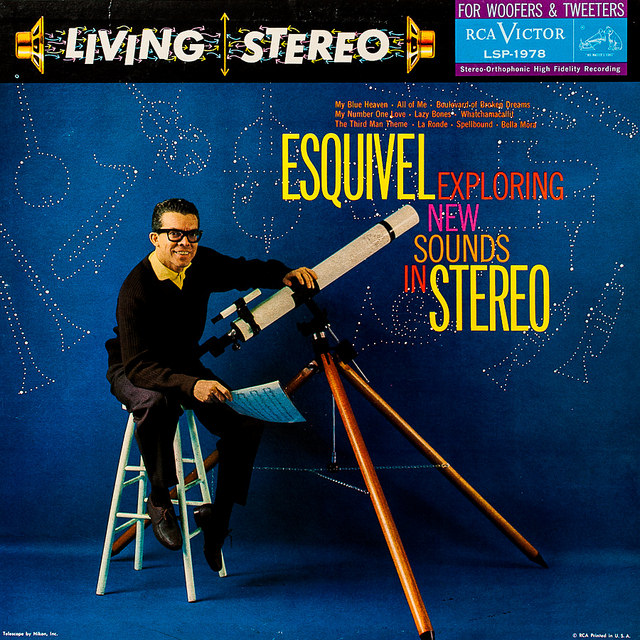
\includegraphics[width=0.5\linewidth]{images/SCP.001.a.record.2.jpg}
	\caption*{SCP-001的封面。唱片封面和无异常的再版封面相同。}
\end{figure}

\bb{项目编号:}SCP-001

\bb{项目等级:}Safe

\bb{特殊收容措施:}SCP-001将被收容于Site-91a的标准低价值收容锁柜中。对SCP-001效应的更多研究将由Site-91a首席数字命理学家Mary Nakayama博士负责。

描述:SCP-001是一张乙烯基唱片,内容为Esquivel发行于1958年的唱片《探索立体新声》(RCA)。该唱片会对将其纳入其中的数据化数字列表产生异常影响。若将该唱片列入数据保存的文本中,它将总是会被第一个列出,即便有意将其调至其他位置也是如此。\footnote{这一效应会扩散到一切形式的数据存储中。迄今受影响设备包括使用级电脑、移动电话、图表计算器。机械式存储设备,如书写或以物理形式表现地列表不会受到其异常效应影响。\label{footnote 2}}

SCP-001在1958年于发行前作为赠审阅副本送给了《公告牌》杂志。其效应一直未被发现,直至20██年十二月,《公告牌》杂志实习生M. S██████在将杂志总部过往审阅唱片的手工文件更新到数据库上时才发觉到其异常并向其上级进行了报告。\footnote{最初这起事件中可能的电子犯罪嫌疑引起了FBI注意。FBI电子犯罪部门内潜伏的UIU特工在发现该物品后将其给了基金会保管。\label{footnote 3}}

正在定位将SCP-001送到《公告牌》杂志的RCA员工。主流收容理论当前认为SCP-001是被用于试尝操控《公告牌》杂志的唱片排行榜,但由于当时该杂志还在使用人工打字,这一企图未能实现。

% =====

\newpage

\tred{▷⦿\slash Procedures\slash 001\slash Past\slash Feb_18,_20██_2.ftml}

\tred{▽⦿\slash Procedures\slash 001\slash Past\slash Feb_18,_20██_2.ftml}

\begin{scpbox}
\bb{基金会数据库修改记录:} \\
很好,真的自己移动过来了。奇怪。有趣。准备继续深入(可能有些隐藏的?)此外,修复了一个打字错误,感谢Dr Amoralles。 \\
- \ii{mnakayama},20██年2月18日11:41 AM
\end{scpbox}

\begin{figure}[H]
	\centering
	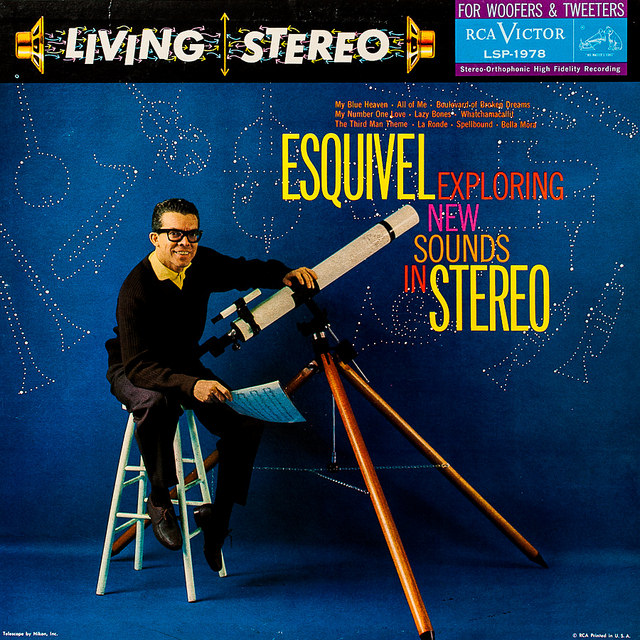
\includegraphics[width=0.5\linewidth]{images/SCP.001.a.record.2.jpg}
	\caption*{SCP-001的封面。唱片封面和无异常的再版封面相同。}
\end{figure}

\bb{项目编号:}SCP-001

\bb{项目等级:}Safe

\bb{特殊收容措施:}SCP-001将被收容于Site-91a的标准低价值收容锁柜中。对SCP-001效应的更多研究将由Site-91a首席数字命理学家Mary Nakayama博士负责。

\bb{描述:}SCP-001是一张乙烯基唱片,内容为Esquivel发行于1958年的唱片《探索立体新声》 (RCA)。该唱片会对将其纳入其中的数据化数字列表产生异常影响。若将该唱片列入数据保存的文本中,它将总是会被第一个列出,即便有意将其调至其他位置也是如此。

SCP-001在1958年于发行前作为审阅副本送给了《公告牌》杂志。其效应一直未被发现,直至20██年十二月,《公告牌》杂志实习生M. S██████在将杂志总部关于过往审阅唱片的手工打印文件更新到数据库上时才发觉到其异常并向其上级进行了报告。\footref{footnote 2}

正在定位将SCP-001送到《公告牌》杂志的RCA员工。主流收容理论当前认为SCP-001是被用于\red{\dd{试尝}}\green{尝试}操控《公告牌》杂志的唱片排行榜,但由于当时该杂志还在使用人工打字,这一企图未能实现。\footref{footnote 3}

% =====

\newpage

\tred{▷⦿\slash Procedures\slash 001\slash Past\slash Apr_1,_20██_1.ftml}

\tred{▽⦿\slash Procedures\slash 001\slash Past\slash Apr_1,_20██_1.ftml}

\begin{scpbox}
\bb{基金会数据库修改记录:} \\
对收容措施进行为期一天的重要修正 ;) \\
- \ii{mnakayama},20██4月1日9:41 AM
\end{scpbox}

\begin{figure}[H]
	\centering
	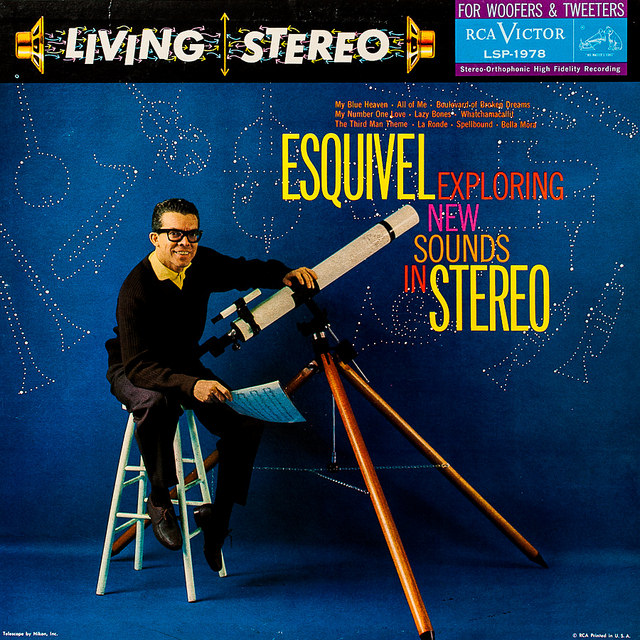
\includegraphics[width=0.5\linewidth]{images/SCP.001.a.record.2.jpg}
	\caption*{SCP-001的封面。唱片封面和无异常的再版封面相同。}
\end{figure}

\bb{项目编号:}SCP-001

\bb{项目等级:}Safe

\bb{特殊收容措施:}SCP-001将被收容于Site-91a的标准低价值收容锁柜中。对SCP-001效应的更多研究将由Site-91a首席数字命理学家Mary Nakayama博士负责。\green{所有Site-91a的2级研究员应当在20██年四月1日于Nakayama博士午餐时间向其支付5美元。}

\bb{描述:}SCP-001是一张乙烯基唱片,内容为Esquivel发行于1958年的唱片《探索立体新声》 (RCA)。该唱片会对将其纳入其中的数据化数字列表产生异常影响。若将该唱片列入数据保存的文本中,它将总是会被第一个列出,即便有意将其调至其他位置也是如此。

SCP-001在1958年于发行前作为审阅副本送给了《公告牌》杂志。其效应一直未被发现,直至20██年十二月,《公告牌》杂志实习生M. S██████在将杂志总部关于过往审阅唱片的手工打印文件更新到数据库上时才发觉到其异常并向其上级进行了报告。\footref{footnote 2}

正在定位将SCP-001送到《公告牌》杂志的RCA员工。主流收容理论当前认为SCP-001是被用于尝试操控《公告牌》杂志的唱片排行榜,但由于当时该杂志还在使用人工打字,这一企图未能实现。\footref{footnote 3}

% =====

\newpage

\tred{▷⦿\slash Procedures\slash 001\slash Past\slash Apr_1,_20██_2.ftml}

\tred{▽⦿\slash Procedures\slash 001\slash Past\slash Apr_1,_20██_2.ftml}

\begin{scpbox}
\bb{基金会数据库修改记录:} \\
这TM这TM这TM是·他·妈·的怎么回事。 \\
- \ii{mnakayama},20██年4月1日12:54 PM
\end{scpbox}

\begin{figure}[H]
	\centering
	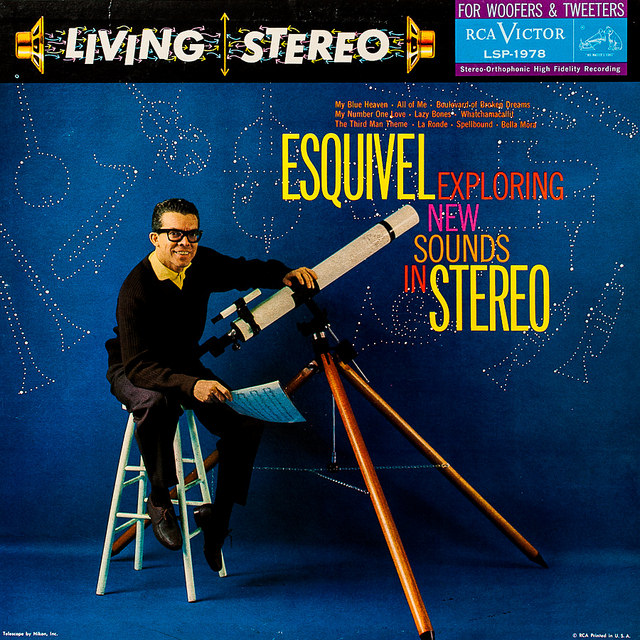
\includegraphics[width=0.5\linewidth]{images/SCP.001.a.record.2.jpg}
	\caption*{SCP-001的封面。唱片封面和无异常的再版封面相同。}
\end{figure}

\bb{项目编号:}SCP-001

\bb{项目等级:}Safe

\bb{特殊收容措施:}SCP-001将被收容于Site-91a的标准低价值收容锁柜中。对SCP-001效应的更多研究将由Site-91a首席数字命理学家Mary Nakayama博士负责。\red{\dd{所有Site-91a的2级研究员应当在20██年四月1日于Nakayama博士午餐时间向其支付5美元。}}

\bb{描述:}SCP-001是一张乙烯基唱片,内容为Esquivel发行于1958年的唱片《探索立体新声》 (RCA)。该唱片会对将其纳入其中的数据化数字列表产生异常影响。若将该唱片列入数据保存的文本中,它将总是会被第一个列出,即便有意将其调至其他位置也是如此。

SCP-001在1958年于发行前作为审阅副本送给了《公告牌》杂志。其效应一直未被发现,直至20██年十二月,《公告牌》杂志实习生M. S██████在将杂志总部关于过往审阅唱片的手工打印文件更新到数据库上时才发觉到其异常并向其上级进行了报告。\footref{footnote 2}

正在定位将SCP-001送到《公告牌》杂志的RCA员工。主流收容理论当前认为SCP-001是被用于尝试操控《公告牌》杂志的唱片排行榜,但由于当时该杂志还在使用人工打字,这一企图未能实现。\footref{footnote 3}

% =====

\newpage

\tred{▷⦿\slash Procedures\slash 001\slash Past\slash Apr_1,_20██_3.ftml}

\tred{▽⦿\slash Procedures\slash 001\slash Past\slash Apr_1,_20██_3.ftml}

\begin{scpbox}
\bb{基金会数据库修改记录:} \\
一些小测试。 \\
- \ii{mnakayama},20██4月1日9:09 PM。
\end{scpbox}

\begin{figure}[H]
	\centering
	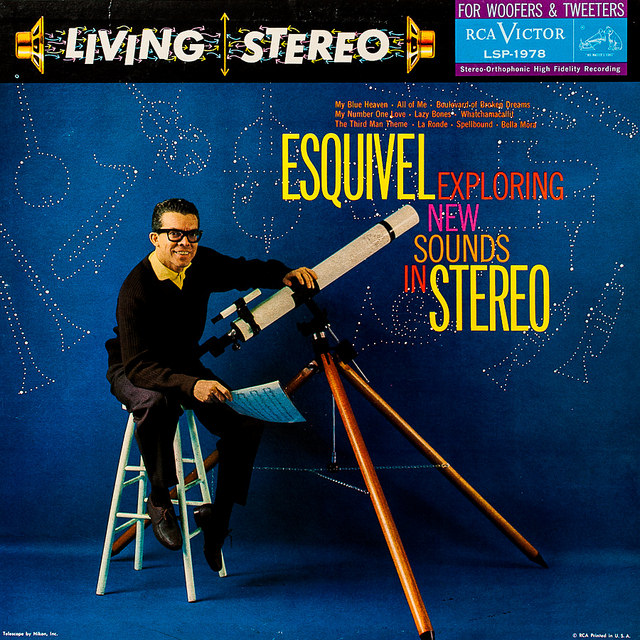
\includegraphics[width=0.5\linewidth]{images/SCP.001.a.record.2.jpg}
	\caption*{SCP-001的封面。唱片封面和无异常的再版封面相同。}
\end{figure}

\bb{项目编号:}SCP-001

\bb{项目等级:}Safe

\bb{特殊收容措施:}SCP-001将被收容于Site-91a的标准低价值收容锁柜中。对SCP-001效应的更多研究将由Site-91a首席数字命理学家Mary Nakayama博士负责。\green{Nakayama博士书桌上的名牌被染成绿色以便于识别。}

\bb{描述:}SCP-001是一张乙烯基唱片,内容为Esquivel发行于1958年的唱片《探索立体新声》 (RCA)。该唱片会对将其纳入其中的数据化数字列表产生异常影响。若将该唱片列入数据保存的文本中,它将总是会被第一个列出,即便有意将其调至其他位置也是如此。

SCP-001在1958年于发行前作为审阅副本送给了《公告牌》杂志。其效应一直未被发现,直至20██年十二月,《公告牌》杂志实习生M. S██████在将杂志总部关于过往审阅唱片的手工打印文件更新到数据库上时才发觉到其异常并向其上级进行了报告。\footref{footnote 2}

正在定位将SCP-001送到《公告牌》杂志的RCA员工。主流收容理论当前认为SCP-001是被用于尝试操控《公告牌》杂志的唱片排行榜,但由于当时该杂志还在使用人工打字,这一企图未能实现。\footref{footnote 3}

% =====

\newpage

\tred{▷⦿\slash Procedures\slash 001\slash Past\slash Apr_2,_20██_1.ftml}

\tred{▽⦿\slash Procedures\slash 001\slash Past\slash Apr_2,_20██_1.ftml}

\begin{scpbox}
\bb{基金会数据库修改记录:} \\
给自己请了个假。 \\
- \ii{mnakayama},20██4月1日9:09 PM。
\end{scpbox}

\begin{figure}[H]
	\centering
	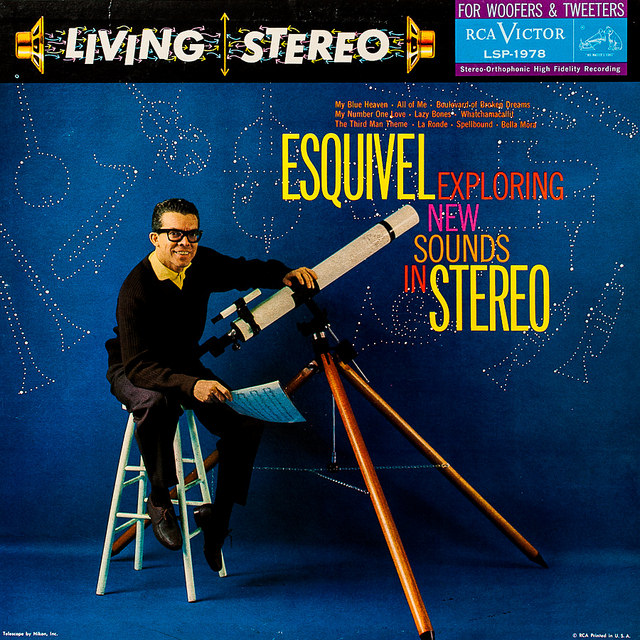
\includegraphics[width=0.5\linewidth]{images/SCP.001.a.record.2.jpg}
	\caption*{SCP-001的封面。唱片封面和无异常的再版封面相同。}
\end{figure}

\bb{项目编号:}SCP-001

\bb{项目等级:}Safe

\bb{特殊收容措施:}SCP-001将被收容于Site-91a的标准低价值收容锁柜中。对SCP-001效应的更多研究将由Site-91a首席数字命理学家Mary Nakayama博士负责。\red{\dd{Nakayama博士书桌上的名牌被染成绿色以便于识别。}}\green{通知所有人员Nakayama博士在20██4月9日前可能暂时不能工作,她已由站点主管Green批准在这期间休假。}

\bb{描述:}SCP-001是一张乙烯基唱片,内容为Esquivel发行于1958年的唱片《探索立体新声》 (RCA)。该唱片会对将其纳入其中的数据化数字列表产生异常影响。若将该唱片列入数据保存的文本中,它将总是会被第一个列出,即便有意将其调至其他位置也是如此。

SCP-001在1958年于发行前作为审阅副本送给了《公告牌》杂志。其效应一直未被发现,直至20██年十二月,《公告牌》杂志实习生M. S██████在将杂志总部关于过往审阅唱片的手工打印文件更新到数据库上时才发觉到其异常并向其上级进行了报告。\footref{footnote 2}

正在定位将SCP-001送到《公告牌》杂志的RCA员工。主流收容理论当前认为SCP-001是被用于尝试操控《公告牌》杂志的唱片排行榜,但由于当时该杂志还在使用人工打字,这一企图未能实现。\footref{footnote 3}

% =====

\newpage

\tred{▷⦿\slash Procedures\slash 001\slash Past\slash Apr_9,_20██_1.ftml}

\tred{▽⦿\slash Procedures\slash 001\slash Past\slash Apr_9,_20██_1.ftml}

\begin{scpbox}
\bb{基金会数据库修改记录:} \\
记录一下将要发生的头衔变动… \\
- \ii{mnakayama},20██4月1日9:09 PM。
\end{scpbox}

\begin{figure}[H]
	\centering
	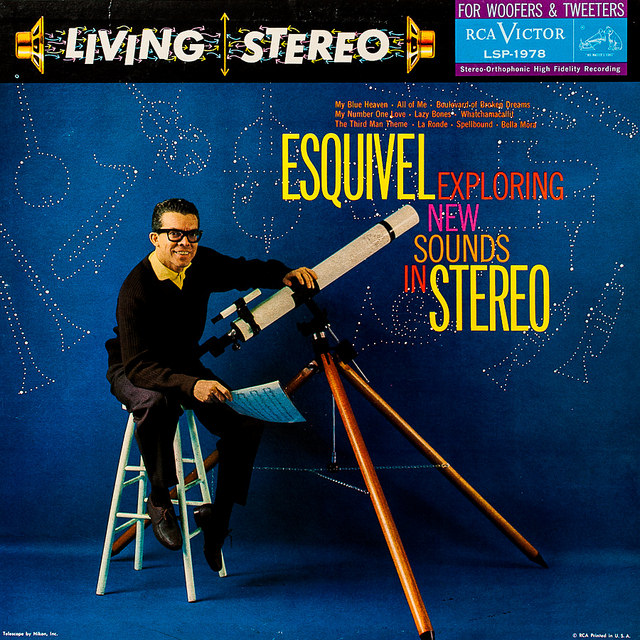
\includegraphics[width=0.5\linewidth]{images/SCP.001.a.record.2.jpg}
	\caption*{SCP-001的封面。唱片封面和无异常的再版封面相同。}
\end{figure}

\bb{项目编号:}SCP-001

\bb{项目等级:}Safe

\bb{特殊收容措施:}SCP-001将被收容于Site-91a的标准低价值收容锁柜中。对SCP-001效应的更多研究将由\red{\dd{Site-91a首席数字命理学家}}Mary Nakayama博士负责。\red{\dd{通知所有人员Nakayama博士在20██4月9日前可能暂时不能工作,她已由站点主管Green批准在这期间休假。}}\green{Nakayama博士,在4月9日以前的Site-91a首席数字命理学家,将在4月9日晚晋升为站点副主管协助Green博士工作。她将独立负责SCP-001项目。}

\bb{描述:}SCP-001是一张乙烯基唱片,内容为Esquivel发行于1958年的唱片《探索立体新声》 (RCA)。该唱片会对将其纳入其中的数据化数字列表产生异常影响。若将该唱片列入数据保存的文本中,它将总是会被第一个列出,即便有意将其调至其他位置也是如此。

SCP-001在1958年于发行前作为审阅副本送给了《公告牌》杂志。其效应一直未被发现,直至20██年十二月,《公告牌》杂志实习生M. S██████在将杂志总部关于过往审阅唱片的手工打印文件更新到数据库上时才发觉到其异常并向其上级进行了报告。\footref{footnote 2}

正在定位将SCP-001送到《公告牌》杂志的RCA员工。主流收容理论当前认为SCP-001是被用于尝试操控《公告牌》杂志的唱片排行榜,但由于当时该杂志还在使用人工打字,这一企图未能实现。\footref{footnote 3}

% =====

\newpage

\tred{▷⦿\slash Procedures\slash 001\slash Past\slash May_3,_20██_1.ftml}

\tred{▽⦿\slash Procedures\slash 001\slash Past\slash May_3,_20██_1.ftml}

\begin{scpbox}
\bb{基金会数据库修改记录:} \\
很好。一切如我所想。我已经准备了好几个星期;现在是时候了。我已经把这个页面对所有人锁定,除了我自己和O5们。我想我是在做一件正确的事。这是我的真实想法。为我祈祷吧。 \\
- \ii{mnakayama},20██5月3日4:11 AM。
\end{scpbox}

\bb{项目编号:}SCP-001

\red{\bd{项目等级:}\dd{Safe}}

\red{\bd{特殊收容措施:}\dd{SCP-001将被收容于Site-91a的标准低价值收容锁柜中。对SCP-001效应的更多研究将由Mary Nakayama博士负责。Nakayama博士,在4月9日以前的Site-91a首席数字命理学家,将在4月9日晚晋升为站点副主管协助Green博士工作。她将独立负责SCP-001项目。}}

\red{\bd{描述:}\dd{SCP-001是一张乙烯基唱片,内容为Esquivel发行于1958年的唱片《探索立体新声》 (RCA)。该唱片会对将其纳入其中的数据化数字列表产生异常影响。若将该唱片列入数据保存的文本中,它将总是会被第一个列出,即便有意将其调至其他位置也是如此。\footref{footnote 2}}}

\red{\dd{SCP-001在1958年于发行前作为赠审阅副本送给了《公告牌》杂志。其效应一直未被发现,直至20██年十二月,《公告牌》杂志实习生M. S██████在将杂志总部过往审阅唱片的手工文件更新到数据库上时才发觉到其异常并向其上级进行了报告。\footref{footnote 3}}}

\red{\dd{正在定位将SCP-001送到《公告牌》杂志的RCA员工。主流收容理论当前认为SCP-001是被用于尝试操控《公告牌》杂志的唱片排行榜,但由于当时该杂志还在使用人工打字,这一企图未能实现。}}

\green{Mary Nakayama,在本文档保存后立刻获得全知与全能,扬升到并成为神。她将超越一切时间,对这宇宙和现实具有完全的统治权。一切事物,一切事物之下的事物以及一切事物之上的事物,都将服从于她的命令。她将得到对在保持和利用这些能力的同时能维持自身意识清醒持续的一切必要心灵性质。}

\green{O5议会成员收到一份说明SCP-001性质的笔记。}

\green{她的家人将收到一份笔记,其中会表明她对他们的爱。}

\begin{scpbox}
Mary Nakayama在5月3日晚六点前从Site 91的宿舍中失踪。至今仍未被找到。
\end{scpbox}

% =====

\newpage

\tred{▷20██年5月3日早存入Mary Nakayama电脑内的文件}

\tred{▽20██年5月3日早存入Mary Nakayama电脑内的文件}

\cl{
致O5议会,

在我十五岁时,我曾吃下过可以杀死我四次的药,给自己灌了一整瓶廉价伏特加,这是那个利用了我又把我抛下、任我心碎孤单的男人唯一留下的东西。

我坐在浴盆里任由热水炽烫我的身体。我闭上了眼睛。

当我睁开眼,我身上的水已经干了。一切安好。我躺在床上。在门边,一个闪烁的身影,发着光芒。盘旋着。它用一个只在我心中回响的声音向我开口说话。它说我有更伟大的事要做。

我再也没有看见过它。但我仍在继续前行。我相信那是上帝降临拯救了我。而,加入基金会后,我还怎么可能不相信呢?还有别的理由能解释为何我们仍存在于此、仍奇迹般地、绝望地、尖叫地活着的事实么?还有别的理由能解释我们世界的根基,我们的一切,竟能经受住这些我们每日面对的异物么?我们被保护着。我每夜向它祈祷指引。我再也未能听到那声音。

我曾触到上帝,那是改变我一生命运的时刻。

但当我在一篇文档上按下“保存”就把自己桌上的名牌变色时,我意识到了什么。万事万物的根基已向我开启。我本可抛下这力量,向你们报告,或者隐瞒它,但…

若这就是拯救我们的关键呢?如果它就是拯救我们所有人的关键,如果就是它在每一天从那些撕碎我们世界脆弱稳定的深渊噩梦手中保护着我们呢? 如果在一个文本里按下“保存”真的就是上帝的诞生呢?

若它不是,那就让我来尝试。若它就是,那就让我来监控它。我会试着将一切纠正。这可能会花些时间。

祝我好运。

- \ii{MN}
}



\chapter[SCP-001 破碎之神]{
	SCP-001 TwistedGears/Kaktus -The Broken God \\
	SCP-001 破碎之神
}

\label{chap:SCP-001.the.broken.god}

\begin{figure}[H]
	\centering
	\fbox{
\includegraphics[width=\linewidth]{images/SCP.001.the.broken.god.png}}
\end{figure}

\cl{

\GG{\bb{根据O5议会指令}}

\Gg{\bb{下列文档描述了Maksur级异常实体}}

信息受5级机密保护。Maksur级信息的泄露被严厉禁止,且将对SCP基金会及其利益造成严重威胁。访问文件的人员须提供5级安保许可,并接受了对AZ109模因危害的预防接种。未能遵照者将在访问文件时立即遭致“携带者奥米茄”模因处决。

\tred{[提交5级安保许可]}

\tred{[安保认知危害启动]}

}

\begin{figure}[H]
	\centering
	\{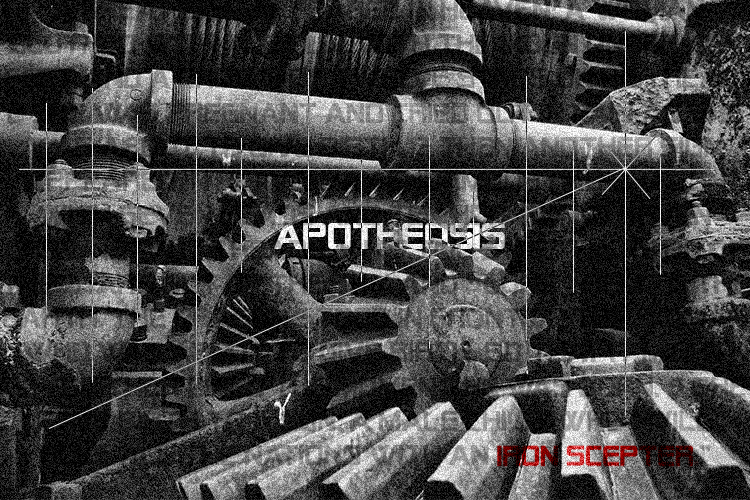
\includegraphics[width=\linewidth]{images/SCP.001.the.broken.god.2.jpg}
\end{figure}

\cl{

\bb{侦测到生命迹象}

\bb{模因接种查明}

\bb{欢迎,监督者}

}

\hr

\begin{figure}[H]
	\centering
	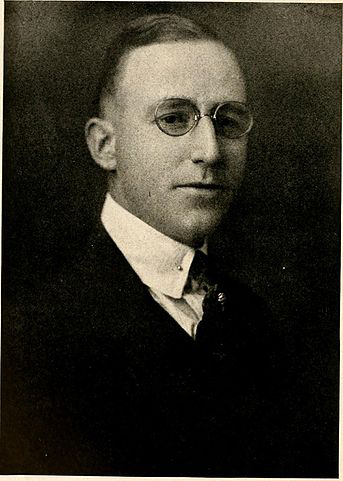
\includegraphics[width=0.5\linewidth]{images/SCP.001.the.broken.god.3.jpg}
	\caption*{Robert Bumaro,破碎之神教会现任领导者。日期未知。}
\end{figure}

\bb{项目编号:}SCP-001

\bb{项目等级:}Maksur\footnote{Maksur分级在1981年由基金会收容委员会联合监督者议会、站点主管议会、基金会伦理委员会联合编入规范。在Maksur级被规范化前,SCP-001曾被编为“Neutralized”,Maksur分级被制定用于替代此不当分级(参加机密委员会记录CA-10931“Neutralized分级在分标准应用中的关联性” CA-10945, “提案:Maksur级”)}

\bb{特殊收容措施:}相关异常项目与SCP-001间存在关联性的信息将在各自文件中被删改。这些项目与破碎之神教会的关联可以保留,但其来源将被删改或模糊处理。

SCP-001的非活跃部件将被留在原地,在其所处区域内禁止任何行船或潜水。平民对SCP-001的察觉将被压制,并使用记忆删除以维持保密。破碎之神教会相关人员若做出寻找SCP-001非活跃部分的举动,将被基金会拘留并审问。关于SCP-001的一切信息,无论是实体还是数据,都将被没收收容。

SCP-001的非活跃部件被预期将保持在无活动状态;然而,若SCP-001出现自发复苏,所有在Site-27, Site-44, Site-90及Site-101附近的活动中机动特遣队单位将被派去采取收容措施。若该事件(当前编为001-登神事件)在现代世界发生,确信当前采取的信息压制措施不足以应对之。001-登神事件极有可能导致一次SK级“破碎面纱”情景\footnote{SK级情景将自动使基金会全部敏感信息备份到自我收容的“深井”站点(当前117、118和119)内最高级安保服务器中。所有非必要人员将接受人工记忆删除治疗,所有主要地方站点将进入全面封锁。当前模型下,该状态尚不确定。},之后将可能是XK级“世界末日”情景。

现存仍活跃的SCP-001部件任何情形下不得进入非活跃部件周围20km内。

\bb{描述:}SCP-001是一系列异常物体之集合,此前曾是破碎之神教会在1942年晚期于墨西哥拉巴斯组装的单一巨型机械实体。这些物体包括\hyperref[chap:SCP-217]{SCP-217},\hyperref[chap:SCP-1139]{SCP-1139},\hyperref[chap:SCP-882]{SCP-882}和\hyperref[chap:SCP-629]{SCP-629}的部分内部零件\footnote{在与破碎教会线人合作收容\hyperref[chap:SCP-629]{SCP-629}后才发现此事。未知这些部件是如何被 Wondertainment博士在基金会及破碎之神教会内部线人不知情的情况下收集到,也不知\hyperref[chap:SCP-629]{SCP-629}自身是否知晓自己与教会的联系。}。完整列表参见\red{这里}。

教会成员将这些异常物体组装在一起,意图以此修复他们信奉的神明。在启动后,据报告SCP-001开始将金属物体整合到自身之中,并开始积极寻找其他异常物体。SCP-001,以及因其被组装而引发的“001-登神”事件,造成了西墨西哥环境发生剧变,并引起了有记载以来最大范围的一次记忆删除施用。在事件后,仍然活跃的SCP-001部件被基金会带回站点收容,非活跃部分则被留在了加利福利亚湾底部,约在23.807269,-108.418369处。

\bb{附录001.01:}描述SCP-001的已收集信息

\begin{scpbox}

\ii{Jorge Castillo神父的陈述抄录,1945年8月}

Fernand是第一个…我觉得,是他们找到心脏后第一个联系我的。他们描述它的方式,还有眼中的狂热,令我迷惑,接着我知道了。我知道他们已经完成了。

在我姐姐的坚信礼后我在周末与Anthony及Salvador见了面…当他们向我展示时我被惊住了。它简直就是一堆齿轮、活塞、发条零件和上油金属部件的混合体,每个部件忠实地相互搅动且没有动力来源。在内部我看到了心脏,一如他们所描述。

它对我说话了。不像你与我这种对话,而是…用图像和感觉。还有痛苦。它处在如此的痛苦中。就像那曾经赋予它生命的火花也让它察觉了自己为何物,又或者不是何物,它只愿再次完整。

愿望这个词也许太过了。不是愿望,更多的是冲动。那造物中的什么东西驱使它向着不假思索、不会动摇的结局前进。他们呈现给我的这个造物和我曾发现并祝福的一切器物都不同。这一个不一样,它有什么地方不对,直到他们完成我才明白过来…

我请求Salvador把它带回\hyperref[chap:SCP-2217]{海岸}拆除,这样是不对的,但他们不可能听进去。在我离开前它已经开始动了。从一头到另一头开始振动,开始走动了。它蹒跚着走过一个扳手,那扳手就变成了它的一部分。他们对我说,“我们的神不破新生了!”

我再没见过他们。

\end{scpbox}

\begin{scpbox}

\ii{1946年对Francis Bollinger的采访}

它不用语词,或者任何语言。它发出金属的声音但同时…当我们靠近图像和概念就涌入了我们心中。你可曾感觉到,当你有了一个思绪或念头-它完全就在那,在你的思维中完整地诞生-但你还是必须去思考与之对应的语言,虽然你在完成句子前就知道了观点?那就像是这样,但却是来自另一个心灵。真正的神之言。

\end{scpbox}

\begin{scpbox}

\ii{2007年对特异事故调查单位特工Trixie Silva的采访}

那里有几个狼-等等,你们知道那是啥对吧?他们就像…就像猎人,为地平线倡议工作。他们在圣玛格丽塔的教堂附近遇到了我们,要我们交出从破碎之神教会那里招来的东西,就像以前我们移交过的亚伯拉罕类物品。

我们讨论起应不应该交出去-我们和地平线的立场有些动摇,更多是最近的事情。我们和当地的破碎教会关系不错,但这些狼…好吧要更有攻击性。我们看着手里的东西,这时候那个女人走了过来。我不知道她从哪里来的。她穿的就像嬉皮士;很瘦,头发上绕着铁链,但她看起来和整个时代完全不合。她眼睛里的凝视,她诡异的笑容,就像她几乎不在那里。

她看着我们拿的东西说她就要这个,噢。我其实并不清楚那到底是什么。一个金属盒子,呼呼又咔嗒地响着,我捡起来的时候边缘还放出了点光。比我原以为的还要亮些。我问这对她为什么那么重要,她说向我展示要比说简单。

她闭上眼低下头。之后她没有动也没有说,我也只好把眼睛闭上了。她把额头靠向我的,但有点分开。我们站了大概一秒,foi muito estranho,接着她突然把下巴往下挪了挪,让我也被向下一拉。

世界在我脚下掉落,我坠了下去。有什么东西在我的思绪里咔哒作响,是一幅双齿轮的图像,先是紧密结合,现在分离开来。我感到脊柱的骨突随我弯腰而伸展,只一步我便同行星这多维的螺丝钉合在一起。它环绕太阳熔炉旋转,被重力锁链所牵引,我们用弹簧无限拉伸的力量,一并飞过这多油的宇宙…

…抱-抱歉。这是一次体验。不,不是宗教体验。但…对。她让我把盒子捡起来,我感觉它好像重了点。我分不清到底是真变重了,还是我感觉它更加…重要了。我把盒子交给她,完全没听到狼或者队友或者上级的声音。

\end{scpbox}

\bb{附录001.02:}1945年6月对被开除的前破碎之神教会牧师Dolorous Randall神父的采访。

\begin{figure}[H]
	\centering
	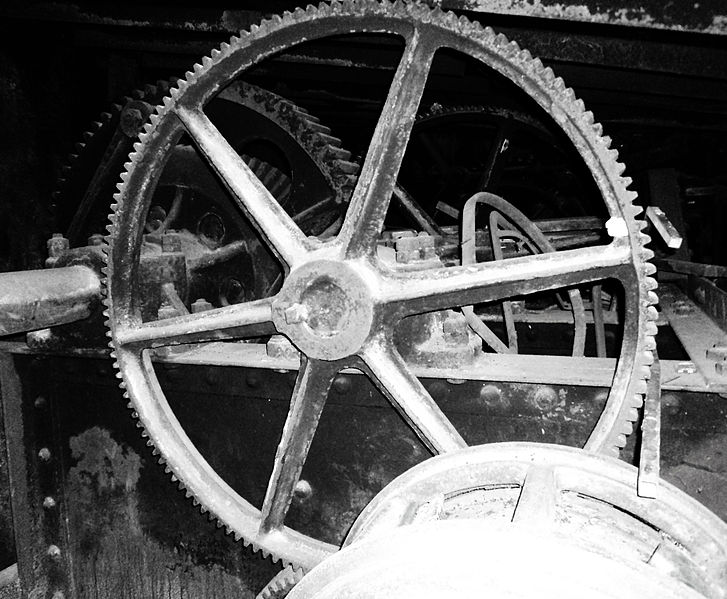
\includegraphics[width=0.5\linewidth]{images/SCP.001.the.broken.god.4.jpg}
	\caption*{在破碎之神教会仓库拍摄的照片。被确信为SCP-001的早期化身。}
\end{figure}


\begin{scpbox}

[多余部分略去]

\bb{Williams:}好了。你早先提到了心脏。他们找到它的时候你可在场?

\bb{Randall:}不,完全没有。那时我在国外,在巴拿马处理一个新任务。我只在事后听说了Ezekiel。

\bb{Williams:}Ezekiel是谁?

\bb{Randall:}Bumaro的一个特工。他身边总有这么一群人,与神协调能感受它的存在,与它对话。Ezekiel曾经发现了个挺重要的器物,Bumaro随后让他加入了。这些特工也是第一批接受改造实验的。如你所想,死了很多。

\bb{Williams:}但Ezekiel没有?

\bb{Randall:}没有。他和Bumaro很亲近,我不知道他会不会拿Ezekiel的健康冒险。这不重要,Ezekiel不需要改造也能与神对话。他就是…能够。

\bb{Williams:}所以Ezekiel对心脏做了什么?

\bb{Randall:}你听Avery说过他们有一大堆器物储备,对吧?这些特工碰过的任何东西,只要他们在其中感觉到了什么,就会被送到拉巴斯和其他的放在一起。大部分都是无价值的,但迟早他们会发现正品。精炼者,那一个-无论你们怎么称呼,一个特工在尼泊尔附近发现了它。他们有了筋腱和韧带等等一切,但都是只是部件。它们都可以自己活动,但不能在一起做什么。

\bb{Williams:}你什么意思?

\bb{Randall:}经典说神会在碎片被带到心脏面前时自行重整。只需要把手臂交给心脏,神就能得到一根手臂。但他们就是找不到心脏。他们(停顿)几个特工曾宣称找到了,但仍是和其他部分一样的无用机械碎片。

\bb{Williams:}Ezekiel在这之中是什么角色?

\bb{Randall:}Ezekiel 是那个告诉Bumaro,如果找不到心脏也许可以自己做一个的人。很快就知道这计划不会持续到夏季过完。我在Ezekiel走后被派去为他们找补给,他们的供应快要耗尽了。

\bb{Williams:}我们的记录显示心脏是被发现的。这不是真的?

\bb{Randall:}当然不是真的。你肯定不能给教众宣道说神把他的部件赐予你然后转身又说其实大部分基础部件都是你自己凭空拼造的。但至少比没有好。他们创造心脏并让它活过来的细节从没向我透露,但我能从蛛丝马迹里得到结论。那年有过一次旱灾,脊髓灰质炎危机又史无前例严重。数千人死亡,都是自然原因。一次可怕的事件,因为注意力都在战争而从未被准确记录过。神啊,但谁说得清呢。

\bb{Williams:}你觉得这两者有联系?

\bb{Randall:}我觉得时机太巧了。而且既然我知道那东西最后变成了什么,我想答案很清楚了。那不是神之心脏,特工。那是完全不同的什么东西。

[多余部分略去]

\end{scpbox}

\bb{附录001.03:}回收到的视频抄录,1942年11月

\begin{scpbox}

\ii{视频回收紫当地纪录电影团体。}

镜头从被破坏的房屋开始,车库周围满是残骸。金属碎片和橡胶条痕迹从车道延伸到沥青路,之后继续到街道上。各种车辆残片散落在街道和沿街上。这些痕迹引向正在将一辆卡车吞入自身底盘的SCP-001。

SCP-001继续向最近的房屋前进,开始吞食排水沟。区域居民逃离现场,多人被SCP-001丢下的玻璃渣和扭曲金属击伤。SCP-001身体的多个部分发出光芒,照在多个跪伏的人影上。SCP-001继续沿街道搜寻更多材料源,其底盘上一个部分变形从主体上落下。

伸出的部分继续变形,形成一个类似人类脊柱及肋骨架的垂直荚体。荚体多处破损,肋骨状突起从中伸出,其余荚体变形为一高约3米的人形实体。光从其头部发出,投在附近的平民上。

金属人形抓起似乎已死亡的平民,将其放入肋骨间的小空间内。肋骨随人形实体靠近第二名试图爬走的女性平民而摆动。实体将挣扎的平民举起放入胸腔内。之后人形实体转身背对摄像头向第三人前进,似乎是女子断手的物体掉落在地。

人形实体的后背上随其收集人体而长出一缓慢增大的赘生物,人形实体的身体大小也随之变小。在吞噬到第六人后赘生物已经大过了人形,使其无法再两足行走。其肢体已收回体内,肋骨伸出使其爬上了附近一栋房屋的屋顶。

它在原地停留了20分钟。球状物外层破裂后从内部裂开,露出三个人形实体。它们看起来是SCP-217感染者,表现出六名被吞食平民的身体特征。其中一名女性头皮上连着锁链,摇晃着另一个似乎已死亡的个体。第三人是一长着发条胳膊的男性,检查自己后跳下了楼顶,腹部着地。它似乎并未因此受伤,令其更为紧张。之后它开始追赶在街道远处吞噬其他汽车的SCP-001。

女性人形注意到了摄像者,开始挥手,但很快停止。它看向SCP-001后跳入后院,离开镜头中。

\end{scpbox}

\bb{附录001.04:}与Robert Bumaro谈话的电话录音。 \\
\ii{备注:下面破碎之神教会一名特工(姓名未知)和Robert Bumaro的电话交谈录音。该次通话记录在1942年12月,由基金会人员在1966年对一处教会据点进行搜查时获得。}

[播放音频]\footnote{
编者\QIS:在\href{http://scp-wiki-cn.wikidot.com/twistedgears-kaktus-proposal}{文章的Wiki页面}上此处是一个Flash控件,点击按钮可播放音频。由于大多数PDF不支持交互操作,所以没有导入。可以点击\href{http://scp-wiki.wdfiles.com/local--files/twistedgears-kaktus-proposal/bumaro.mp3}{这里}访问该音频。
}

\begin{scpbox}

[通话开始]

\bb{Bumaro:}你好?

\bb{Agent:}祝福您圣父。

\bb{Bumaro:}Dmitri?

\bb{Agent:}不。

\bb{Bumaro:}哦,当然。祝福你,孩子。小主如何了?

\bb{Agent:}日渐强壮。我们已将他从办公室后面挪入了附近的仓库。

\bb{Bumaro:}喂过他了吗?

\bb{Agent:}如您要求。

\bb{Bumaro:}很好。你何时去Puerto Peñasco?

\bb{Agent:}本周内。我们就等下列车。

\bb{Bumaro:}可能还得快点。几周前拉巴斯被突袭了一次。我们有三个人没有被找到。基金会活动越发活跃在-(暂时挂断)

\bb{Agent:}圣父?

\bb{Bumaro:}(对背景的某人)明天,明天。

\bb{Agent:}圣父?

\bb{Bumaro:}是的。我们曾期望他们北上,但他们却去了西边。小挫折。

\bb{Agent:}那安全屋呢?有将近一百件其他器物在那里,而且—

\bb{Bumaro:}(打断)小挫折。他们不知道在哪,就算他们知道了,这也不是他们的优先项目。他们的眼线,还有他们在世界上的其他眼线,都注视着欧洲。只要他们的目光落在那里,就不会发觉我们的完成直到已经无力阻挡他。

\bb{Agent:}这,嗯,还有其他事想问您,圣父。

\bb{Bumaro:}是的?

\bb{Agent:}我们的神,呃…太饿了。我们似乎无法满足他,我们得到的供给不—

\bb{Bumaro:}(再次打断)问题是什么?

\bb{Agent:}圣父,我们的…主在吃他自己的住所。我们无法劝服他停下,不能和他讲理,它-

\bb{Bumaro:}胡说。虔诚的心可以与神直接对话。当他靠近时你不能听到他的话吗?没有感觉机械在你心中运转?或者连在眼前呼吸鲜活的神也不能让你坚信?

\bb{Agent:}不!圣父,不是这样,是-

\bb{Bumaro:}我不会再听了。这么多年,我们祈祷、期盼神在我们面前不破新生。现在,他已展现了自己。我们知道神会对虔诚之心开口。如果你要告诉我,你们中连虔诚到能与神沟通的人都没有,现在就告诉我把你们换掉。

\bb{Agent:}我们的信念依然坚定,圣父。请您原谅我的无礼。我只是迷途了。

\bb{Bumaro:}那就自己反省。我担心你的信念。去找个弟兄,找个信念比你坚定的,让他去和主对话,告诉他保密的必要。我们的主将会理解,毫无疑问。不破之神是一位理智的神。

\bb{Agent:}是的,祝福您圣父。

\bb{Bumaro:}祝福你,孩子。

[通话结束]

\end{scpbox}

\bb{附录001.05:}增补报告,1943年12月 \\
\ii{下面是对基金会Site-74指挥官Mark Peterson的采访。主管在001-登神事件前驻扎于墨西哥城,事件期间与拉巴斯的基金会人员一同在站。}

\begin{figure}[H]
	\centering
	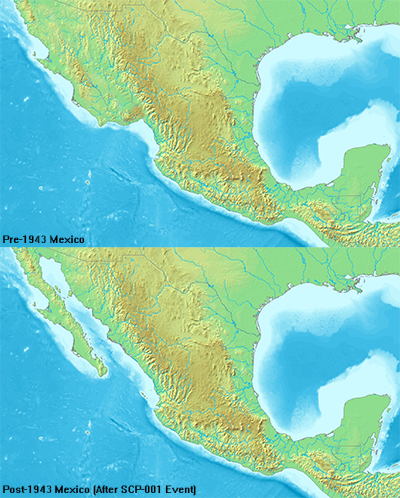
\includegraphics[width=0.5\linewidth]{images/SCP.001.the.broken.god.5.png}
	\caption*{001-登神事件前后的墨西哥}
\end{figure}

\begin{scpbox}

\bb{Director Cornwell:}从头再来一遍,我们在记录。

\bb{Commander Peterson:}好。关于教会活动的第一次报告是在41年,但那时候还都是非常小的事。我们刚刚完成了北部边境附近的外勤行动,正要准备把资产搬去亚特兰大准备法国的任务。我们已经接到命令,去收回一些他们不愿意被德国佬抢去的敏感物品。他们还准备派出我们整个部门去完成此事。领导不确定罗斯福会不会打电话为我们留下充足时间协同美军,所以我们必须得单独前进。

\bb{Director Cornwell:}你为何留在拉巴斯?

\bb{Commander Peterson:}我完全是偶然在那。我们的一辆列车取道往拉巴斯的陆路,也许是要顺路去取回一些军备。结果那趟列车本来是要北上的。所以突然之间大部分格兰德河以南的领导层就跑到了拉巴斯来,回想起来从整体效果看这倒可能帮了我们大忙。

\bb{Director Cornwell:}你何时首次听闻001-登神实体?

\bb{Commander Peterson:}(笑)耶稣啊。现在他们这么叫那东西了?那个机器,我猜, 我们第一次听说,是有本地活动频繁的风声,在…我猜大概得是一年多以前。我们在42年10月到了拉巴斯,所以…对,听起来没错。我们搞的第一个确凿证据是在一辆… 难民车?虽然这么叫着很傻但我想是准确的。他们在十月末来到拉巴斯,说整个镇子都被盖住了。他们没有真正的解释什么,就是一直说“la máquina, la máquina”, 你知道的,“机器”。顺便这就是我们那么叫它的原因。我们还完全不清楚那应该是个什么。

\bb{Director Cornwell:}那你和该实体的第一次接触呢?

\bb{Commander Peterson:}好吧,铁路停止运营了,如果你是这意思的话。我们听当地警方说北边出了事故,列车不会再往边境开了。这对我们来说可是大问题,我们可不能坐着几辆车向东走到山脚小镇为止。它们大多都和单独的铁道线完全挂钩,我们本可以就那么走。但是大东西,那些列车要去拉巴斯拉的东西,不能动。所以我们得等着。之后DeMarco想出个注意,派支小队沿铁路看看堵塞在哪,我们能不能清理掉它。他自己领队。

\bb{Director Cornwell:}特工DeMarco怎样了?

\bb{Commander Peterson:}你他妈知道他出什么事了Bill。

\bb{Director Cornwell:}为记录。

\bb{Commander Peterson:}好吧。我们三天没有收到回信,于是准备把剩下的领导层送去东边免得再等了。但五天后DeMarco的一个部下回到了营地。他精神混乱,说着“吞世怪物”,还有其他所有人都被盖掉了的话。他们是被盖掉了不是吗?我知道那时候它还不是最后那么大,但也不是可以应付的东西。DeMarco…

\bb{Director Cornwell:}你没事吗?

\bb{Commander Peterson:}没事。他试过想杀掉它。但接着他也许明白了我们之后才弄明白的事;我们不可能收容这东西。世界上没有哪个洞大到能装下它,或者有什么盒子是它吃不掉的。但这对他没意义了,其他跟着他去的人都是。那机器不关心这些。

\bb{Director Cornwell:}你什么时候第一次看到了它?

\bb{Commander Peterson:}十二月。在我们蹲守期间,我加入探索队溜过去看个究竟。它已经…我是说,你看过它对边境做了什么。我从来没看过大成这样还能动的东西。就感觉是一座活动部件堆成的山染黑了天空,好像它是在烧那些被它铲进胸口的东西一样。然后它又小了!它… 我不知道。我们都接受有XK-事件准备训练,但这个超出或者说在我们受过的任何训练之外。它就是无敌的。我们知道我们是去送死,那东西要杀了我们,只是个时间问题。

\end{scpbox}

\bb{附录001.06: }收集到的基金会通信 \\
\ii{备注:下面是拉巴斯驻扎基金会人员的书面通信摘录,在001-登神事件后回收于临时站点。姓名已隐去。}

\begin{scpbox}

亲爱的███████,

我甚至不知道这封信能不能送到。列车全停了,但指挥官说还能把信送出去。我希望确实如此,希望你能读到。

这里的天空已经暗了好几周了。每天北边都有烟飘来,呼吸都很困难。这里还是没有室内水管,除了我们公司的另一些人外都不说英语。

我们还是不知道我们在这里干什么。我一直听说要修铁路,但为什么不去北边?不是北边的铁路坏了吗?

\end{scpbox}

\begin{scpbox}

今天有个男人来到镇上,基本上半张脸都被煮过一样。他就像个死人,对谁都不回应。他走到镇中间就倒地了。在医务室醒来后,他变得很激动。说什么山一样大的机器还能和你说话。说那里有人从各自家里跑出来,把自己扔到它身上。说他们被碾碎,像是在草坪修剪机下面跳一样。之后他就死了,没人知道怎么回事。

\end{scpbox}

\begin{scpbox}

山脉在我们面前被撞碎。我们看到一个身影从烟中立起,缓慢笨重但势头恐怖。它不是像野兽一样爬行或是人一样走动,而是靠着几百万齿轮转动推进,就如钢铁的眼镜蛇。它的身体向前伸出,进入烟中,高过我们所能触及。在它的胸口里我看见有火在跳动,就像地狱的熔炉。它来到我们北边的山前,却没有停下或是绕路,而是就这么穿了过来,把山峰全部吞噬。它身处一条长胳膊,将整个村庄抓起塞进口中。我看到人们随家园被抹去一并走向死亡,和其他人一起投身地狱中。接着它叫了,不是齿轮的嘎吱或机械的轰响,而是在我们的心里。我能在心里听到它。它在嚎叫。

\end{scpbox}

\begin{scpbox}

\bb{指令:}中央指挥部,Site-001

\bb{敬礼:}█████████████

临时站点损失。拉巴斯成为废墟。机械实体被收容。大规模地理改变。XK已避免。申请记忆删除支持。

\end{scpbox}

\bb{附录001.07:}采访GOC中尉“归来者” \\
\ii{备注:下面是对全球超自然联盟中尉、代号“归来者”的事后采访摘录。采访记录及全部抄录由基金会特工在1992年的协商情报交换中获得。迄今“归来者”的身份仍然未知。}

\begin{figure}[H]
	\centering
	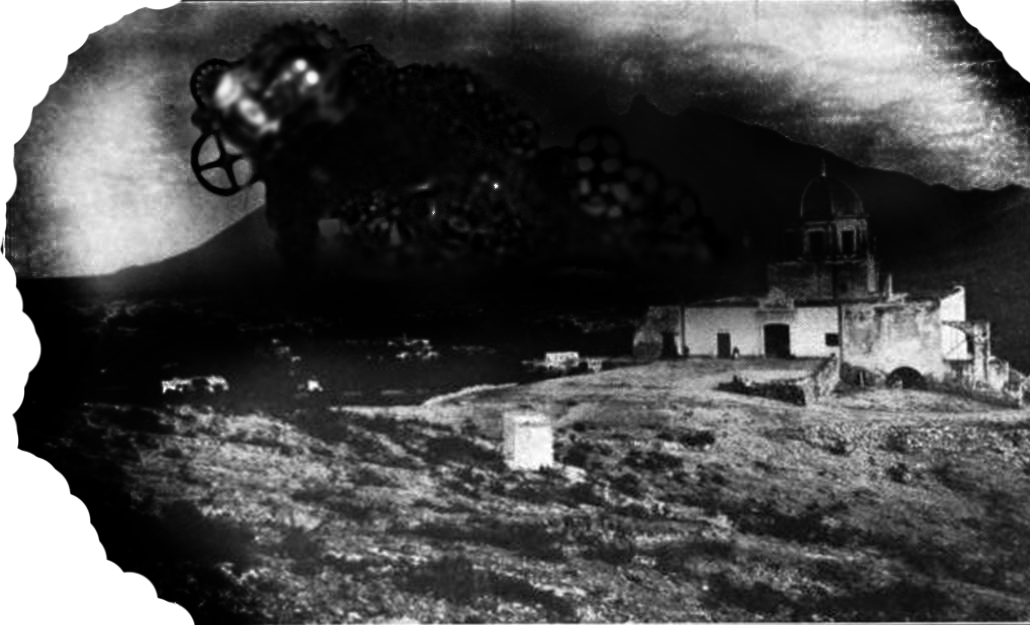
\includegraphics[width=0.5\linewidth]{images/SCP.001.the.broken.god.6.png}
	\caption*{SCP-001,照片拍摄于事件后且严重受损,拍摄者未知}
\end{figure}

\begin{scpbox}

基金会特工里流传着一些故事,就是那种白头老兵在长夜值岗或者在小房间里讲给新兵蛋子的故事。我不知道是谁开的头,但我知道他们现在还在讲。已经半个世纪过去了,他们确实还是对的,你就是可以给他们如此信任。他们说,“你知道么,GOC杀了神。”

但新兵就会说,“不,这不是真的。神被收容在Site-管他是哪呢。反正GOC没有杀过神。”接着他们就会讨论起被他们锁在某处的绿型,那个说自己是基督教上帝的家伙。但这时老兵只会摇摇头,笑而不语。因为他们都知道。

他们都知道在1943年,在末日之中,基金会只能眼看着GOC拯救世界,什么都做不了。

隐喻枪是在希腊海岸边的一座岛上被发现。我甚至不记得它长什么样了,我记得的只剩下记忆删除留给我的那一点模糊回忆。但我本能地觉得它不是你以为的那么重。

为什么记忆删除?那时候我跟着地区部署的分遣队,显然有一块碎片让它造成了心智影响。我模糊地觉得有什么不对,所以我听了他们的话。我不记得它长什么样,我也想不起来它是如何毁掉那么多大陆的。该死,我只记得它何时发生,知道这事的唯一原因还是前后地图的变化。但我还是能感觉到,我的本能说,事情本不该如此。我们站在一个愤怒的复仇神面前,而它做的全部事就是祈求我们杀掉它。

我们全都是如此乐于履职。

\end{scpbox}

\bb{附录001.08:}记录到的视频抄录 \\
SCP-001的较早图像,在附近城镇的撤离中拍摄

\ii{备注:下列是回收的视频录像抄录,长约30秒。抄录在回收后不久被批准,当前视频本身已经损坏无法解读。视频的声音被调节到可接受状态,可在下方播放。\footnote{译注:此处有语音。}}

\bb{回收音频:}警告:声音极大。

[播放音频]
\footnote{
编者\QIS:同前文注。音频文件可点击\href{http://scp-wiki.wdfiles.com/local--files/twistedgears-kaktus-proposal/Apotheosis.mp3}{此处}访问。}

\begin{scpbox}

\bb{00:01:}记录在镇上开始。许多建筑倒塌着火。有明显的剧烈地震活动。

\bb{00:03:}视频移向SCP-001。大小在视频中难以辨认,但该实体占据了整个镜头。它正在缓慢移动。

\bb{00:09:}SCP-001被看到将大块土地移入自身中。偶尔有火焰从实体中迸出。

\bb{00:15:}天空似乎被闪电照亮,可以听到空袭海妖的声音,SCP-001上方的云层突然分开。\hyperref[chap:SCP-2399]{SCP-2399}出现,其下部轻度损坏。可以看到基金会迫击炮从上方飞过。
\bb{00:20:}一发炮弹击中SCP-001。没有造成可见损伤。

\bb{00:22:}SCP-2399的下部开始发蓝。

\bb{00:24:}SCP-2399发出明亮光束击中SCP-001。SCP-001剧烈反应并向 SCP-2399抓去。

\bb{00:26:}巨大爆炸。视频内容不可见。

\bb{00:30:}附近人群尖叫,视频结束。

\end{scpbox}

\bb{附录001.09:}SCP-001的无效化

\begin{figure}[H]
	\centering
	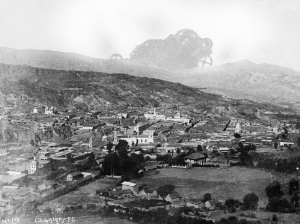
\includegraphics[width=0.5\linewidth]{images/SCP.001.the.broken.god.7.png}
	\caption*{SCP-001的较早图像,在附近城镇的撤离中拍摄}
\end{figure}

于1943年7月17日,全球超自然联盟的特工联系了基金会在墨西哥拉巴斯的主管,请求支援对001-登神实体所在地的运输。基金会特工迅速部署飞机救援GOC人员。抵达后,特工描述称他们获得一个特殊的异常器物,并有可能被用于阻止001-登神实体行动。

在抵达拉巴斯的三天后,于1943年7月24日,全球超自然联盟派出一名特工携带该特殊器物去往001-登神实体所在地。在1943年7月25日早上,在001-登神实体抵达太平洋海岸时另一个巨大的机械构造体\footnote{之后编为SCP-2399并在文件中给予合适掩盖故事。}出现在其上方。该实体的来源未知。

在SCP-2399出现后的事件记录不完整且可能不准确。此次遭遇的结果是SCP-001被消灭。SCP-2399消失,之后以损坏状态出现在木星,当中原因至今未知。

SCP-001剩余的非活跃部分,即一团巨大分散的机械部件,留在了加利福利亚海湾底部。在从非活跃的结构体中取出SCP-882后,剩余部分坍塌彻底停止活动。

在001-登神事件后,对该区域居民进行了代号“下加利福利亚”的大规模记忆删除行动。此次行动因SCP-001周围厚重的黑烟得到支持,当前历史记录将此事件描述为一次森林火灾。大量精力被投入在修正区域地图及搬迁失所平民上。出于对大规模记忆删除规范的需要,多个实验性神经变形器被使用\footnote{特别是U级、UN级和UP级记忆删除,当前都已被终止。},因对其副作用缺乏认知,估计此举造成不少于200万人在001-登神事件后的十年内死亡。

\bb{附录001.10:}收集到的全球超自然联盟文档 \\
\ii{备注:下列文件由POI-004D/001(参见附录001.12)交予基金会人员。当前未知POI-004D/001如何获得此文件。}

\begin{tcolorbox}[colframe=black, boxrule=0.5pt, colback=white, center upper, leftright skip=0.12\linewidth, breakable]

\begin{figure}[H]
	\centering
	
\includegraphics[width=0.6\linewidth]{images/SCP.001.the.broken.god.8.png}
\end{figure}

ATTN:Darius将军

物品回收报告

\bb{编写:}Van Pelt中尉

\bb{C.O:}Baghram上校

\bb{报告长度:}57页

\bb{报告概要:}1942年12月30日,一个具异常性的游荡人形实体在希腊海岸外的小岛附近被巡逻员发现。该实体,宣称没有名字也不能流利用英语交流,携带一个棒球大小的小型立方体器物。实体似乎为女性,其头皮上连着几根钢链。

实体最初愿意交出所带器物(编为AR-213),但很快出现敌意并开始说话。实体对中队人员发出生命威胁,击倒两名人员,随后被Dixon军士制服。实体提及墨西哥西部,要求将其释放把该器物带去那里。

更多调查发现SCP基金会在该区域的活动越发频繁,同时还有一些轻微地理异变。在aghram上校指令下,第二团看守该实体(编为EN-340)开往异变地点。在舰船停靠美国边境后,EN-340开始变得消极,显然不适且心理失常。

建议返回后,在处决前对EN-340进行更多心理评估。一旦对AR-213的分析完成,器物将被送往苏黎世焚毁。

报告附于此以供考察

Lt. R. Van Pelt

第二团

全球超自然联盟维和部队

\end{tcolorbox}

\bb{附录001.11:}Ruberson特工的陈述,1944年1月

\ii{备注:特工Aaron Ruberson在收集SCP-001器物时正驻扎在站。因大部分基金会高级人员被派往参加收集,他被要求进行事后陈述。报告原先存放在 Site-17,之后被加入另一与SCP-001相关的机密材料中。未知是否有其他人员知晓此报告,或者有任何副本被制作。下面是陈述摘录。}

\begin{figure}[H]
	\centering
	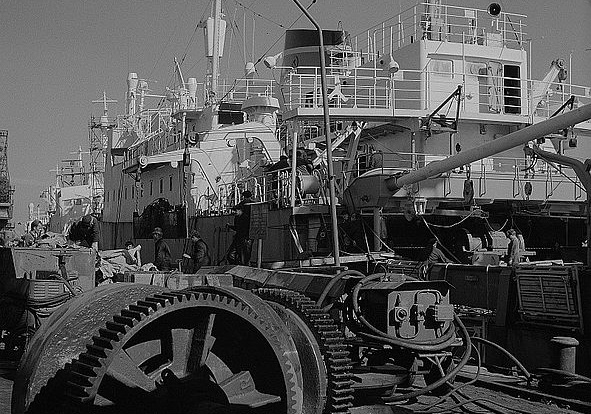
\includegraphics[width=0.5\linewidth]{images/SCP.001.the.broken.god.9.jpg}
	\caption*{SCP-001的非活跃部件正在被装船送往收容。}
\end{figure}

\begin{scpbox}

我们先把能从海岸拿走的拿了。小东西、齿轮滑轮还有活塞,就这一类。大部分都是垃圾,但还在抽动和旋转。它们还是有生命的。这些小零件大概在几小时后死透,但几周后我还是能听到那些大碎片在搅合。就像砍掉鸡头那样。

重要的部分,那些已知是真正教会器物的,被我们打包运往拉巴斯的列车运走。我数了数,基督啊,也许得有一百个?每个都是异常器物。车站有些小伙子笑话说就为存这些东西他们怕是得修个新站点。

幸运的是我们把伤亡压得很低。大部分人都只是在机械附近有些懵,就像是不能把手臂拿开一样。Rodriguez的手被压了,我们只好把他送去当地诊所处置。我觉得整个过程里就有一起死亡。一个我们雇来的当地人帮忙潜到海湾下给那个心脏捆上绳子,好让我们把它拉出来。我没看到,但我听说了。说他们发现他的头被碾烂在两个活动部件中间。还说看起来他是自己把自己推进去的。

但我不知道,我没亲眼看见。我倒是有看到标签。

你知道的,当某地制造了什么产品,为了便于辨认其产地,这些家伙总会找个大片金属刻上名字然后在部件一侧给它贴上吧?我们在其他部件上看到了不少这种东西,都是它在一路向海吃过去的途中收集的。不过教会器物都不是这样。它们和其他所有东西一样嗡嗡响,但是没有标志。你站在这些东西前就能感觉到什么,像是安详。整个感觉就像,它感觉很平静。像是解脱。

除了那个心脏。当我们终于把它搬上海湾,因为天气原因我们把它留在岸边放了一天。有些当地人开始发痒。说他们听到声音,不愿意靠近。不管多少钱都不干。只有等到北边的基地派来更多支援才能把它弄上船。

我…伙计我不知道。我见到过各种的这些东西,但我的模因抗性还是很高的。我为这个任务通过了不少测试,一切良好。但我无法抵抗围绕那心脏的另类感觉。我不知道可不可以说听到了什么,但…好吧,标签。我们把它搬上船向北准备离开的时候我第一次看见了。我那时候还没想到要说什么,甚至都没往心里去,知道我看到了其他一些文件。接着船在风暴中沉了,我们丢失了心脏,整个时间我一直在想着那该死的金属标签。接着我想我发现了。那根本不是教会的东西,Johnny。
标签上写的是“工厂所有”\footnote{因近距离检查SCP-882的困难性,这些言论尚未得到证实。}。

\end{scpbox}

\bb{附录001.12:}对POI-004D/001的采访 \\
\ii{备注:下面是2009年对POI-004D/001的采访摘录,此人自称为一此前未知的破碎之神教会分支成员。联系在特异事故调查单位协助下进行,他们曾与POI-004D/001有过互动,详情记录在附录001.01中。}

\begin{scpbox}

所以,给我说说你觉得你们知道的事。

明白了。

有趣。

好吧,你们倒也不是全错。在现在这个时候也是值得称赞的。我感觉你们忽略了几个关键细节,以及高看了某些自认健忘症患者给你们的情报。

那就让我直说好了。

GOC并没有杀死耶和华,虽然他们自傲地如此宣称着。他们消灭的也不是破碎之神。确实,那确实是它的碎片之一,但你会给我个轮轴再把它叫成车么?噢,所以你们把几个部分凑在了一起。也许有引擎了,但仍然不是车。

神比那要更为简单。神是万物。从最大的星到最小的尘。每个小部分,对它们自己都是微不足道的。做着它们应做的事。切合在一起,相互咬合。这全都是宇宙机械的一部分。

这机械的面貌,在某种程度上,就像是一种比喻。一个理念。但我肯定你们也知道,理念是强大的。它们从无中创造出有,或是将已有的加以改变。神的一小束火花闪过,象征成为真实。在一颗生命如此丰盛的星球上,你们产生了无数理念。

你可能要问,“为何要叫它破碎之神?”可能的回答有几个。和翻译问题一样简单的事。被虔信者重新解释得具体了。“破碎”只是对某个更微妙词语的糟糕翻译吗?神是在大爆炸中破碎了吗?如果是这样,它为何破碎?若它被修复又会怎样?

这些问题我一个都无法回答,但你们已经有了答案。到最后,无论神曾经是什么都不重要了。重要的是,对你们而言,它必须保持现状。“破碎”。神知道。那些更强大的部分,传统教派视为圣物的机械部件,它们知道它们本不该成为一个整体。就算迫使其合体,用异己的力量驱动,它们也知道自己本真为何。怪兽的啃咬会向自我毁灭行动,派出更小的实体来完成工作。GOC没有杀死它,它们是从它自己手中接过了枪,扣动扳机后又宣布这是自己的功劳。

问题在于,人类作为神的一部分太过渺小,无法去记忆。无法记忆他曾经是怎样。于是那些如Bumaro的人就要发明新路把我们推向奇点。

因为这是将要发生的。你可看到毁灭者的下部?在43年的遭遇前那里就是损坏的。如果你仔细看去,你将看到伤疤离动力核心越来越近。这次它甚至伤到了让它能藏进现实夹层的什么东西。最后那怪兽将胜利。它迟早会毁灭毁灭者,吞噬它,然后用它的力量吞食一切。我是说一切。神将后回归到唯一的完形存在,一个奇点,然后碎裂。只有这次它可能有了某种异己力量在其中。工厂之锈。Daevite王之血。第五教会,Wondertainment,街上随便某个有足够火花成为现实扭曲者的人。它们也会参与宇宙的重塑,并完结所有这些的次轮回。

不,这并不令我困扰。这是注定之事,这必将发生。谁又能说这不是已经在发生了,而你们的人是赢家呢?也许人类自身才是赢家。但这并不意味着我要反对关掉它,让主轮回继续。

是的,这有可能。我知道上次你们未能伤到那怪物,毁灭者也许到下次需要它的时候仍不能修复自己。但谁说你们不能支援它呢?或者模仿那些寻求重筑神明的人,得到外来协助呢?一同努力,没有什么不可能。

分离,我们是破碎的。但团结,我们将为神。

\end{scpbox}


\chapter[SCP-001 过去与未来]{
	SCP-001 Kalinin - Past and Future \\
	SCP-001 过去与未来
}

\label{chap:SCP-001.past.and.future}

\cl{

编者\QIS :本篇翻译尚不完整,暂时不予收录。}

\hr

目前相关文档:

\begin{itemize}
\item \href{http://scp-wiki.wikidot.com/kalinins-proposal}{英文Wiki原文}。
\item \href{http://scp-wiki-cn.wikidot.com/kalinins-proposal}{中文Wiki翻译},文中后续文件链接到的页面均不存在。
\item \href{http://bbs.scp-wiki-cn.org/posts/list/27826.page}{论坛翻译},此版本用的英文原文暂不明。
\end{itemize}


\chapter[SCP-001 一致意见]{
	SCP-001 Wrong - The Consensus \\
	SCP-001 一致意见
	\footnote{编者\QIS:这个脚注用于去除一个我还没搞明白的\TeX 排版问题,只要标题的最后一个字不是汉字就行,为了美观就加了个脚注\label{foot:fix}}
}

\label{chap:SCP-001.the.consensus}

\definecolor{ftwoftwoctwo}{HTML}{F2F2C2}

\begin{scpbox}[colback=ftwoftwoctwo, center upper]

\bb{基金会记录与信息安保管理部通知}

一年二度安保更新:项目编号随机化已启动。直至安保更新完成,所有文件将锁定。要进行紧急更新,请访问紧急数据归档系统(EDAS)。

— Maria Jones,RAISA主管

\end{scpbox}

\hr

\begin{scpboxcmd}

> 1908个项目存留。项目编号“SCP-001”锁定。 \\
> 识别到1个带有搜索字段“SCP-001”的文件。

> 文件~'SCP-001'被选中。 \\
> 开始自动项目编号随机化。 \\
> 扫描带有搜索字段“SCP-001”的文件…

\end{scpboxcmd}

\hr

\begin{figure}[H]
	\centering
	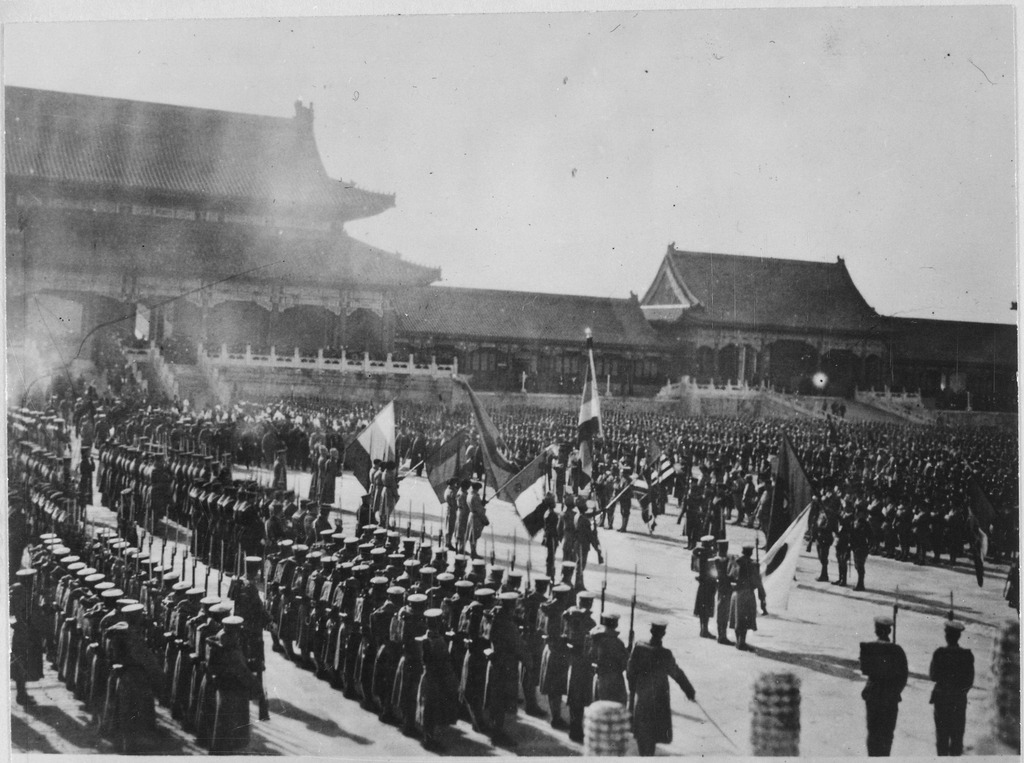
\includegraphics{images/SCP.001.the.consensus.jpg}
	\caption*{北京紫禁城,\red{SCP-001}的定义及紫禁城公约的通过在此完成。}
\end{figure}

\bb{项目编号:}\red{SCP-001}

\bb{项目等级:}Euclid

\bb{权限分级:}5级

\bb{特殊收容措施:}\red{SCP-001}当前无法被便利控制或收容,未知其是否会在未来发生。因此已采用应对方案。该方案由紫禁城公约的以下章节组成:

\begin{enumerate}
\item 依照紫禁城公约章节I,预防并最小化可能造成\red{SCP-001}或类似事件的情形。
\item 在紫禁城公约章节I实施后,依照紫禁城公约章节II及III安排组织过渡及联合。
\end{enumerate}

上述紫禁城公约章节不得变动,除非得到O5议会全体一致通过。

描述:\red{SCP-001}是一已经发生的CK级重构情形,造成过往某一迭代的现实变化,生成了当前的现实。从第一人称观察记录来看,\red{SCP-001}发生于前现实的公元1900年6月1日。\red{SCP-001}致使所有关于超自然大战\ii{i}(前一现实中称其为第五次超自然大战)的因果、事件、记载和记忆被删除并替代为各种异常或非异常的平行记录。

基金会关于超自然大战\ii{i}的文件采集自十三名非异常人类的传闻记录,这些人员因被称作“部分性\red{SCP-001}免疫”的现象而保有对前一现实的记忆。部分性\red{SCP-001}免疫的原理未知,依照O5议会指令不会对其进行评定。依照O5议会指令,对其他具有部分性\red{SCP-001}免疫人员的辨识工作被无限期暂停。

下面是在超自然大战\ii{i}中的事件及其在当前现实中可能的对应类似事件;参见文件OWi获取完整列表。

\tred{+ 查看列表}

\tred{- 隐藏列表}

\begin{longtable}{m{0.2\linewidth}m{0.3\linewidth}m{0.35\linewidth}}
\hline
超自然大战\ii{i}事件 & 描述 & 当前现实对应 \\
\hline
\endhead
\hline
\multicolumn{3}{r}{\small{接下页}}
\endfoot
\hline
\endlastfoot
“第五次超自然大战”的称谓 & 发生于公元19世纪的全球性战争,由发生于欧洲(拿破仑战争)、东亚(狄瓦族征服战)及美洲(美国内战)的三起独立冲突组成。战争中公然使用异常物体,造成了一次IK级全球文明崩溃情景。 & 与“拳乱”同时发生于中国北部的冲突事件,起义组织义和团据称在此事件中使用了某种未命名异常。\par 虽然对异常的使用非常微小,O5议会仍在知晓异常现象的诸组织中倡议将“第五次超自然大战”作为对此事件的正式称呼,全球超自然联盟在基金会-GOC的1953年峰会中正式承认了这一主张。\\
拿破仑一世加冕 & 拿破仑皇帝在加冕后宣布新诺斯替教为法国国教,欧罗巴为国家守护神。& 教皇庇护七世将拿破仑加冕为“法兰西皇帝”拿破仑统治期间从未有发现过新诺斯替主义和欧罗巴女神崇拜的表现。 \hyperref[chap:SCP-2515]{SCP-2515}是对此的唯一证据。\\
狄瓦族东亚征服战	& 东亚大部分地区被名为\overtextnote{\hyperref[chap:SCP-140]{狄瓦族}(\footnotesize Daevites)} 的类人文明入侵。征服从中国黑龙江省及吉林省开始。& 没有对应事件。\hyperref[chap:SCP-140]{SCP-140}中的记录显示狄瓦文明被蒙古人消灭于公元13世纪。然而,确实曾在中国黑龙江省及吉林省发现过狄瓦文明器物。\\
南北战争 & 美利坚合众国及美国南部邦联间的内战。名为“工厂”的团体向双方都提供了异常军备支援。在南部邦联政府转移后,战争逐步扩展到墨西哥、中南美。& 未发现工厂参与南北战争。战争规模始终局限于美国大陆地区。\\
图基教平定运动 & 第零反邪教军团针对骚扰\hyperref[chap:SCP-2833]{Vātula}(被视作与英国东印度公司对抗狄瓦族对印度入侵的共同战力)的犯罪集团图基教的镇压活动。& 由《1836-48年图基教及土匪镇压法案》委任的镇压活动,确认有新欲肉教参与。\\
梵蒂冈神秘及预言圣裁庭 & 知晓异常现象的组织,隶属于梵蒂冈圣座。在拿破仑进攻意大利半岛时,其成员逃难到南美、非洲自由邦及中东。& 圣物部(梵蒂冈圣裁庭下属部门)叛逃到意大利统一政府,组建了基金会前身组织之一“皇家基督教圣物办公室”。\hyperref[chap:SCP-1732]{梵蒂冈圣裁庭在公元1964年与基金会合并}。\\
“墨西哥帝国”的建立 & 自称Cem Anáhuac,是阿兹特克帝国的后继者。\hyperref[chap:2155]{其对象及由其产生的媒体具有模因能力},被用于政府周边邦国,如德克萨斯、危地马拉、萨尔瓦多和洪都拉斯。& 墨西哥第二帝国在法国干涉下建立,由皇帝马西米兰一世统治。据传他在被处决前曾与一个SCP-2155-1个体安排了联姻。\\
东田纳西会议 & 由东田纳西的合众国支持者组成,在田纳西州参与南北战争后脱离该州。由此形成的\hyperref[chap:SCP-1328]{富兰克林州}被承认加入美利坚合众国,也是合众国一方中唯一一个自南部邦联脱离的州。& 东田纳西会议在南方军占领东田纳西后告终。西弗吉尼亚自弗吉尼亚州脱离,并在南北战争后作为一个州保留。\\
太平天国运动 & 在狄瓦占领下的中国南部发生,由一名为洪仁坤的奴隶策划发起,他自称得到了名为\hyperref[doc:2481]{“龙母”}的神明启示。在起义首都太岁京(被太平军占领前为南京)被狄瓦族攻陷后遭到镇压,全城居民被屠杀。& \hyperref[chap:SCP-089]{SCP-089}告知的一起S级事件,由女王陛下超常控制收容基金会及黑庄园的联合探险队处置解决。洪仁坤在此利用了对基督教的自我改造,并给自己改名为洪秀全。\par 未发现欲肉教或基督教相关异常活动涉及此事。南京在被太平军占领后改名为天京。\\
土默特部大屠杀 & 一名狄瓦族奴隶在狄瓦占领下的蒙古地区系统性屠杀了150000名蒙古人。报告称\hyperref[chap:SCP-076]{此奴隶}手持两把带刃武器并具有某种再生能力。起义者的尸体被狄瓦军队以未知目的回收。& 一起“金丹道之乱”类似地造成了150000名蒙古人被屠杀,但此事是由中国秘密结社金丹道造成。金丹道在前一现实的存在因资源有限而无法确认。
\end{longtable}

\red{SCP-001}的起因和源头未知,也无法确认。未知\red{SCP-001}或类似事件在此之前是否还曾发生,也未知其是否会在未来发生。此外,未知\red{SCP-001}是否是CK级重构情景的典型或非典型表现。若\red{SCP-001}或类似事件已经发生或是将要发生,推测大部分(甚至全部)人类和/或智能实体将对此事件及其发生前的事件不会保留记忆。无法确认部分性\red{SCP-001}免疫是否能在未来的\red{SCP-001}或其类似事件中有效。

\red{SCP-001}的定义由O5议会以投票5-4-4完成,紫禁城公约于公元1901年9月7日签订。

\bb{附录1:}紫禁城公约摘录

\bb{章节I:基金会}

\begin{whiteboxbb}

下列组织将自各自资助方中解散并脱离关系,其人员及资源将进行合并:

\begin{itemize}
\item 女王陛下超常安保收容基金会
\item \ii{黑}庄园
\item 沙皇先知会
\item 德意志帝国秘传战团
\item 美国安保收容倡议
\item 帝国侵犯事件委员会
\item 皇家基督教圣物办公室
\item 荷兰东印度公司特别调查董事会
\item 内阿非利加探索队会社
\item Borja y Aragón军备骑士团
\item 阴阳局
\item 中华异学会
\item 第零反邪教军团
\end{itemize}

它们将被取而代之联合为一个统一组织。

该统一组织的使命是控制并收容各种异常事物,以保护人类免受此类事物威胁。

同意将该统一组织的称谓定为“基金会”;其他替换称谓(如“学会”、“组织”、“机构”、“前哨”)曾被提议但否决。上述十三个基金会构成组织自此后称作“基金会前身组织”。

\end{whiteboxbb}

\bb{章节II:O5议会}

\begin{whiteboxbb}

基金会的临时执行管理部门将是来自各前身组织的十三名人员组成的执行议会。

上述十三名执行议会成员将依照下列标准选择:

\begin{itemize}

\item 在各基金会前身组织居领导职位
\item 保有关于第一次超自然大战\ii{i}的记忆

\end{itemize}

未来的执行议会成员不再要求满足上述两个要求。

同意将执行议会的称谓定为“O5议会”;其他替换称谓(如“监督者委员会”、“5级议会”、“O5指挥部”)曾被提议但否决。

O5议会的功能将为促进各前身组织间的初步过渡。

每名O5议会成员将以罗马数字编号,从一排列到十三。

今后其他并入基金会的组织机构不得在O5议会存有代表。

\end{whiteboxbb}

\bb{章节III:关注组织}

\begin{whiteboxbb}

知晓异常现象存在而不受基金会管控的各组织机构被编为 \overtextnote{“关注组织”(Groups of Interest)}。

基金会对各关注组织的默认对策是促成其人员和资源的解散、终止和/或将其吸收。

\end{whiteboxbb}

\bb{附录O5-(1-13):}继任笔记re:\red{SCP-001}。 文件根据登录的O5账号显示。

\definecolor{dafadnine}{HTML}{DAFAD9}

\begin{scpboxc}[colback=dafadnine]

验证登录权限。识别到管理员优越权(代号嚎叫黑月)。\\
展示所有文件。

\end{scpboxc}

% \begin{whiteboxbb}

\begin{scpbox}

欢迎您O5-1

致我的继任者,

作为\red{SCP-001}的主要编辑者,我已写下了你所需知晓的一切。在\red{SCP-001}后,只有我们十三个知道它,我们各自代表各自的前身组织。当然,我们命定要指挥和联合为基金会。

你可以从我们的投票看出,我们在北京争论时有关于\red{SCP-001}的另外两种版本。它们最终被投票否决,但二和十二仍在基金会历史上留下了自己的记号。遗憾的是十二有限的英语水平让它选中了相对通俗化的分级名词,与二和我刚好相对。无论如何,我们召开首次O5会面的倡议将在已写下的所有SCP文件中被记忆、发扬。

至于基金会之使命,我希望你和你的同事能继续我们的工作。

\end{scpbox}

\begin{scpbox}

欢迎您O5-2

致我的继任者,

桑塔亚纳曾说,“忘记过去的人必将重蹈覆辙”。现在,整个世界都忘记了过去。但它会重蹈覆辙吗?它会的。

在第二次世界大战期间,不是又有一个威权独裁者恐吓欧洲,中国人再一次被屠杀了吗?当然,细节些许不同,美国也在战争中保持了完整。也许内战在你的一生曾再次发生,或者很快就要发生。又或者缩减为一次小冲突。 工厂仍然留存,但它只是幻影。

异常的产物自身也会是异常。\red{SCP-001}和它的世界不是例外。一点一点,世界在毁灭、重蹈覆辙。每有一个SCP不(或者只是最低程度地)在我们的控制下,这个进程都要继续。在那之前,系统里都会有混乱存在。曾经,我提议指引世界回到原来的状态,但其他人不愿赞成专横暴行。最终,我认了。 没必要为我的观点斗争。没什么能改变这个过程。

除了等待,不必采取任何行动。或者简言之,“Keter”。

\end{scpbox}

\begin{scpbox}

欢迎您O5-3

致我的继任者,

异常与正常—都取决于合意。今日的异常可能是昨日之正常,反之亦然。九未能发觉的丑闻就是一例;出逃狂在合意认为它不再成立后便不再是异常。

将合意适用在\red{SCP-001}。对其余的世界,超自然大战从未存在。它们只对那些知道异常的人存在。对知道异常的人,超自然大战\ii{i}并不存在。只有十三人幻想它存在,那可能就是\red{SCP-001}。

然而,议会建立了我们自己的合意,我的观点在它宣告之时也随之转变。我们多数决定应该对所有异常事务建立管控秩序,而不是觉得我们自己才是问题。这只是第一批达成的合意之一,我们能左右世界将什么视作正常,什么不是。也许是他们造就了你所成长的这个世界。

所以,请记得这些。合意有其价值,要正常就要被合意所接纳。

\end{scpbox}

\begin{scpbox}

欢迎您O5-4

致我的继任者,

只有少数人在两个第五次超自然大战中都上过前线,我是其中之一。我对官方的第五次超自然大战非常失望,毫无疑问那是缩了水的。那些拳匪根本无法与狄瓦族和发条信徒相比。就算是把几乎其他所有机构、教派都变成了我们的敌人,地下结社无论如何不能与全面战争相比。

也许这又是我心头的年轻热血在抱怨。\red{SCP-001}发生后它频繁的发作,就像在北京我一时冲动投票支持了二的提议。我并不关注他古怪的理论。我只想战斗。已经做出了如此多的牺牲,我也做出了惨重牺牲。不能让它们结束在这平静的日子里。但现在,我老了,平静也快找到我了。但你在此继续战斗。别让它在平静中终结。

\end{scpbox}

\begin{scpbox}

欢迎您O5-5

致我的继任者,

你现在知道了这世界曾经因为一起无法控制的事件而免于彻底毁灭。而正因其不可控制,我们无法保证它不会再次发生。或者会不会如我们愿地发生。我们不能依靠\red{SCP-001}这样的不确定。

作为一个物种,我们已经主宰百兽,踏遍大地。许多技艺已为人所掌握,而它们曾经都只是幻梦。世界的复苏只是另一件有待主宰的事情。若世界能让自己倒带,我们也能做到。

在我们的联合之下,我所展望的\hyperref[chap:SCP-2000]{杰作}将可能成为现实。它可能已被利用过,或是建构仍在继续着,但\red{SCP-001}一旦就绪就将不可逆转。凭我们的意志,人类将主宰永恒。

\end{scpbox}

\begin{scpbox}

欢迎您O5-6

致我的继任者,

我们同意\red{SCP-001}曾经发生, 但我们不知道这是否是\red{SCP-001}唯一一次发生。它会不会再次发生?一定要世界濒临毁灭才会出现吗?要到什么程度才足够?这跨现实的记忆保留又是为何,这是怎么回事?为什么是我们?它能复现吗?问题表如此继续。

这非常现象的不确定级别显然需要得到量化。‘Euclid’是对此的提醒,即对于\red{SCP-001}还应当有更多了解。我想你应当有此动力,毕竟有着基金会倡导科学方法论的熏陶。收容与保护不能是终点;知识才是。但第一届议会的大部分人害怕探索,想着要么抛弃它要么预防。哪一种都不能真正解决问题。

但你可以为解决问题做自己的贡献。只有你能看到这些,并访问到我仅有的少许发现,所以就让它成为你的出发点。愿你得到结果,为\red{SCP-001}带来有意义的资料。

\end{scpbox}

\begin{scpbox}

欢迎您O5-7

致我的继任者,

官方而言,只有13个人对\red{SCP-001}免疫。但还有另外一人,Jibril Mani。他是为土耳其皇廷工作的一名顾问,我在因拿破仑逃难到君士坦丁堡期间遇到了他。他无比好客,我们很快成了朋友,尽管基督教世界和伊斯兰世界历来敌对。我们待在一起直到\red{SCP-001}来临,突然之间我回到了罗马。

在现在的世界,他想办法找到了我,我知道他还记得我们曾经的友谊。我们在见面后大谈对超自然一战的记忆。我邀请他加入北京的聚会,和其他还记得战争的人一起,但他礼貌的拒绝了。

Jibril更愿意保护他的朋友和族人,特别是我们知道中东正一片混乱。他对一和他的势力心存怀疑,但我也无法为此责难他,只能尊重他的选择。那之后我们分道扬镳了。当我获得O5-7的头衔,Jibril告诉我他\hyperref[chap:ORI-oria.hub]{会回到伊朗召集自己的人手}。

就像他希望保护他所爱的人,我的使命是这世界,我会保卫他。

P.S. 出于尊重,我决定不对议会报告Jibril的事。我希望无论Jibril和议会最终各自成立了什么样的组织,它们都不要发生冲突。我们只愿保护。

\end{scpbox}

\begin{scpbox}

欢迎您O5-8

致我的继任者,

你可以从投票中猜到,对\red{SCP-001}的来头有过三个选择。一的提议无疑是唯一选择。其他人太愚蠢了。二基本上就想让我们去当无政府主义者,十二则觉得我们是一帮疯子需要服点东方神药。不必了,谢谢你们两个!

我们大多从一开始就在收集异常物件,所以基金会对多半前身组织而言并无多少不同。而对剩下的一半,关注组织的制度会让所有人意见一致的。

你应该已经做这些工作好些时候了,所以我希望你继续下去。

\end{scpbox}

\begin{scpbox}

欢迎您O5-9

致我的继任者,

\red{SCP-001}是现实的重构,这是我们的合意。所以\red{SCP-001}是现实扭曲。二宣称现实会不可避免地逆转回去以纠正世界,这和斯克兰顿在此问题上的著名观点颇为相似。不过,后者认为这种复原是由现实扭曲者引发的。控制智能存在可能非常困难,虽然某些学者认为一台\hyperref[chap:GOI-grant.request.for.the.manufacture.of.devices.to.regulate]{引擎}也许可以在理论上提升概率。这种前景带来了希望-这已知最庞大的现实扭曲活动是可逆的。

而当此事发生,世界真的复原到之前的状态-和我在非洲自由邦、并未真正受到IK级情景波及的家园一起完成。它可能也是过往世界里唯一安全的避风港。这样的稳定在\red{SCP-001}之后失落了,最终我要在一片更不友好的条件里工作。

虽然我并不喜欢一的观点,基金会目前到确实是更好的环境。这是个思考如何实现斯克兰顿想法的好地方,或者至少资助有这能力的某人。尽管我已投入了财力人力,进程依然缓慢,我已接受了事实,我可能再不能拿回所失去的东西了。

但你能,如果\red{SCP-001}再次发生。你应该继续用你所能的方法研究下去, 你不应该像我这样失去了自己的东西。没有人应该这样。

\end{scpbox}

\begin{scpbox}

欢迎您O5-10

致我的继任者,

十三个团体一起创立了基金会,但并非我们每一个都地位平等。比如十二所代表的异学会并未得到清朝的承认。而我这边也同样在走下坡。我们的名号属于一位猎巫人,但我们从未见过真正的女巫。19世纪末的Borja骑士团说成是关注组织会更恰当。要不是我对超自然大战\ii{i}的记忆,它就会一直如此。

当一说出他的大计划,我却对如何对抗异常心存怀疑。每一代骑士都是前一代的影子,结果如何呢。在超自然一战中,我记得我的骑士们被拿破仑的发条兵全歼。他们过去(现在也是)并未准备好迎接超自然之战,或者是对抗恶魔及法师。接受一的提议意味着再一次送他们惨烈赴死。作为他们的大团长,我不能送他们去死。

当投票结果不合我意,我曾差点考虑不签署合并条约。但当我听到八提议促进我们新命名的基金会联合起来,这种想法便烟消云散。那之后,我决定我的骑士们至少应该有意义地在与怪物的战斗中死去,而非作为牺牲品。

我们所有人终有一死。就让它对你责任之所在有所意义好了。

P.S. 其实考虑到这一切,其他前身组织的资源也确实能让最后一代骑士们比前一批更优秀。

\end{scpbox}

\begin{scpbox}

欢迎您O5-11

致我的继任者,

恭祝你为基金会服务。我想你是一级一级爬上这个位置的,而不是我这样因为品德第一上位。你的品德一定让人震惊,不同于我。

在超自然大战\ii{i}期间,京都陷落于狄瓦族之手,孝明天皇和议会大部分人罹难。将军和他的特务们逃去了虾夷。我是少数逃离京都的幸存者,但这只是因保命而胆怯。我最终为自己的选择悔恨,耻辱将我压倒。死不能令我解脱。至少孝明天皇在这新世界驾崩地要略微平和。

这决定了我在北京的投票,我们是出现了幻觉,记忆删除能治好我们。其实我只是想遗忘而已。但合意已成,我不被容许遗忘。一坚持我们命定要合作,议会里没有人站到我们这边。

知道还有人和我一样后,至少好受了些。三、七和十三带来了非常积极的影响。我的继任者啊,我并不了解你这一代O5议会的同事们,但他们将是你的忠实盟友。谨记。

\end{scpbox}

\begin{scpbox}

欢迎您O5-12

致余之继任者,

汝必尝闻除忆秘法,经年,其效亦有所\hyperref[chap:SCP-3000]{增},然回溯其源,实为基金会诸秘密之一也。余将释其原本。

除忆秘法者,初为孟族术师之密。余与彼族女约为婚姻以得之。初,余见幻景烦扰,欲以秘药去之,然今知其为超自然大战\ii{i}之记忆也。

未及药成,十一通信于我,曰有幻景类同。未几,余便知有外邦人若干见得同样幻景,且约为集会于京城。余身为医者本当见人病愈,便劝其勿为蛇足之举以求身全。然同会诸君不以为然,议以西洋民主投票之法定夺之。余之见自然为其所弃。

然除忆秘法不为其所弃。五以其略同于\red{SCP-001},可逆人之记忆,实为可用之方也。由是,除忆方不以余见为疗病之药,而用之于平民百姓见异事者,除其记忆。

有所不幸,孟族主母不容洋人窃其族方,余等遂将孟族一部列之于最初之关注组织。其一族下场大抵同于义和拳,但余一二小辈携一不甚解之\hyperref[chap:SCP-484]{秘方},奔逃香港。

汝自当效汝才干于议会,然既已谋得此职位,汝定当已效英才于此也。

\end{scpbox}

\begin{scpbox}

欢迎您O5-13

致我的继任者,

\red{SCP-001}说只有十三名前身组织的领导者才对其效应免疫,事实并非如此。只有十二人。

一和我已经认识了几十年,我欠他许多。自然,当他要我投下决胜一票,我答应了。他把狄瓦人入侵印度的事告诉给我以完成骗局。当那里都是我不知道的东西,我只会怪罪不列颠不愿对我的军团坦诚相待。

我想你现在该对这头衔为耻,我敢说我们这可能有三个不同的基金会在相互斗争。对我,这是让欧洲人正视问题、让我赢得优势的机会。自那时,我已作出许多补救,不让他人落入我的处境。

所以,向我保证你会以自己的意愿去投票,而非他人。

\end{scpbox}

% \end{whiteboxbb}

\hr

\begin{scpboxcmd}

> 扫描完成。识别到40个“SCP-001”。\\
> 开始随机编号生成…

\end{scpboxcmd}


\chapter[SCP-001 黎明将至]{
	SCP-001 S. D. Locke - When Day Breaks \\
	SCP-001 黎明将至
}

\label{chap:SCP-001.when.day.breaks}

\begin{scpbox}

你发现了那条通道,正隐藏在距主干道一英里外的天然洞穴内。

无需钥匙卡,通道之门是敞开的。

这里的气味闻起来和它们一样。但愿它们已经离开了。你走的太远,你无法回头了。

一条平滑的小径从洞口向内延伸,通向站点深处。也许会有些血液或粪便 – 或是那些东西涂抹的污渍,这可说不准。所以你得小心避开。

你仍能收到求救信号,它是从昨天开始的,无论是谁 – 你祈祷他们能够生还。

你的脚步声回响在空荡走廊之中,每一步都仿佛传达自另一个世界,就好像你并非在黑暗中独行。

电梯停留在底层 – 故而你沿楼梯下行,直至B5层:Keter控制区,你穿过几个空收容室,它们曾能造成的恐惧和动荡早已不复存在。

如果你运气够好的话。

这条路将你带往大厅一侧的办公室 – 那里正是信号的来源。门没上锁,但被什么东西卡住了,你抬起脚,用尽全力踹了过去。

在你能看清屋里的事物前有个东西从你左侧的角落里冲了出来,你的第一反应是“狗”。

但它曾蛰伏在天花板上。

你躲入房间,砰地关上身后的门。此处一片漆黑,你是安全的。你脱下外套,摘掉头盔。在经历了如此之多的事情后却死于中暑将会是莫大的耻辱。

唯一的应急操作灯旋转在塑料外壳之中 - 每隔一秒便在房间中洒下暖橙色的灯光,仿佛房间本身的脉搏正有节奏地律动着。

门后随意搁置着 – 一个路障,你环顾四周,脏衣服和吃了一半的食物,尽管临近厕所,角落里却有个盛满排泄物的桶。北面墙上的气动室将向房客提供必要的生活物资。

你的路终止于房间角落某个令人作呕的泥潭,你看到了三个药瓶 - 检查发现这是三种不同的鸦片类药物,它们都是空的。

桌上有台电脑,靠近终端,你可以清楚地看到电源指示键闪烁着微弱的灯光。

你坐下,开机。

\end{scpbox}

\hr

\cl{

\Gg{紧急协议激活。删除级别保护措施。完全访问权限。}

控制。收容。保护。

\par

\par

加载中...

加载中..

加载中...

加载中..

加载中...

加载中......

}

\begin{scpbox}
你听到门外传来了脚步声,一步步愈发沉重,下一步又接踵而至。
\end{scpbox}

\cl{

加载中...

加载中..

加载中...

加载中..

加载中...

加载中..

加载中...

加载中..

加载中...

正在验证...

..

...

}

\begin{scpbox}
黑影由地板和门边的缝隙悄然渗入,被光线映照地轮廓分明。
\end{scpbox}

\cl{

..

...

..

正在验证...

..

...

..

...

..

正在验证...

..

...

}

\begin{scpbox}
你紧张地屏住呼吸等待着,希望它只是路过。然而你的心跳此刻在你自己听来,却震耳欲聋地暴露了你的位置。
\end{scpbox}

\cl{

请等待...

..

...

..

..

...

请等待...

..

...

..

请等待...

..

...

..

}

\begin{scpbox}
阴影消失了,你的呼吸松懈下来,正在这时,屏幕亮了起来……
\end{scpbox}

\par

\cl{

打开文件

\Gg{🔥自动化安全系统通知代码235(ASSN-235)🔥}

检索SCP-001文件当前迭代时出错,您正在查阅版本\#3 ,可滑动至页面底部查阅较新版本。

}

% =====

\newpage

\tred{开启文件:SCP-001修订版\# 3/12:(1)音频文件}

\tred{隐藏修订版}

\g{\bb{修订版\# 3/12更新于1312日前}}

\hr

\begin{figure}[H]
	\centering
	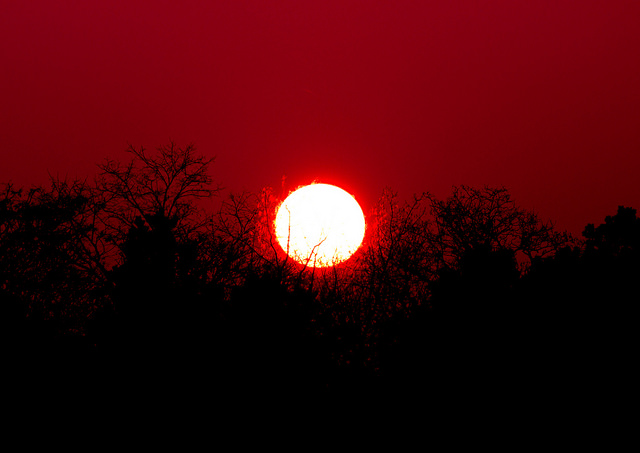
\includegraphics[width=0.5\linewidth]{images/SCP.001.when.night.breaks.jpg}
	\caption*{SCP-001激活后数分钟,拍摄者未知。}
\end{figure}

\bb{项目编号:}SCP-001

\bb{项目等级:}Apollyon\footnote{译注:abad,希伯来语意为破坏者,希腊语译为apollyon,英语译为abaddon,指圣经启示录中的地狱使者亚巴顿,又称无底坑的使者。}

\bb{特殊收容措施:}由于其性质,SCP-001无法被收容。SCP-001事件幸存者将驻扎在安全设施中并彼此保持联系,鼓励人员采取任何可行的手段前往Site-19。

希望进行户外活动的幸存者必须保证周身覆盖防护服;最好是多层防护,应尽可能避免徒步旅行,城市 – 也指通常意义上的人造建筑可提供最大程度的庇护,需规避树木繁盛区,空乘是所有出行方式中的最优选择。

暴露于SCP-001的人员将被视为损失,受连累者将被遗弃,请不要尝试安乐死。

应不惜一切代价避免SCP-001-A组成规模庞大的集群,已证实电导武器在固定情况下有一定作用,故可用于自卫,燃烧器也可正常使用,迄今为止,冷冻弹药是最有效的。

测试显示SCP-001-A是相对安全的可消耗品,但只能被视为没有其他选择的情况下的最后手段。由于SCP-001-A可在消化系统中重构,因此短时间内仅能消耗少量,以防止堵塞。

驻扎于Site-19的人员从事有关世界殖民化的研究,载具经过专门设计,内部不得被光线穿透。

\begin{scpbox}

\begin{scpbox}

对于那些失去了家人,或者上帝啊,失去了孩子的人们 – 我对此深感,深感遗憾。但你必须坚持下去,不要让他们白白死去,我们还有时间。

人类仍可能拥有未来,到Site-19来,我们需要尽可能多的援助。

学会拥抱黑暗,朋友们,我们惧怕光明。

\hr

\hfill - \ii{The Administrator}

\end{scpbox}

\end{scpbox}

\bb{描述:}SCP-001是在事件[系统错误]\ii{数据丢失:ec172,请联系系统管理员。}后对于太阳的编号。此次事件发生二十四小时内造成约68亿人类伤亡。SCP-001的影响似乎不是经由紫外线产生,而是暴露于可视光谱(~390至100nm)导致。即使身在月光下也同样如此。

当活体接触太阳产生的可见光时,将从接触点处开始液化,效果持续扩散,直至整个生物体完全转化。从外观上来看,同蜡融化类似。转化时间很大程度上取决于生物体的暴露程度和其大小。尽管发生了这种重组,生物体也不会死亡。

转化完成后,这些生物体(SCP-001-A)将呈凝胶状,它们会尝试活动,尽可能使自己固定在可令人联想起先前样貌的形态,这种努力可取得一定程度的成功。

植物通常保持物理惰性,但仍能够进行光合作用并产生氧气,可飞行的生物丧失飞行能力,动物具有意识,在未被吸收至集群的前提下,行为与往日无异。人类则保有少许智慧和记忆。

暴露于SCP-001的生物性异常受到同样的影响,曝光可抹消其曾表现出的全部异常。

由于它们的物质组成,SCP-001-A个体可通过彼此接触进行分子水平上的联接和混合,这似乎不会对个体造成任何痛苦和伤害,但组成的体积可抑制其运动。自SCP-001-A事件以来,大多数个体已集聚为这样的集群,似乎不存在最大融合上限。

融合后的生物质是无定形且混沌的,集群生物将在半液态中转换形态 – 其中肢体和身体质量将在短时间内周期性升高,随后恶化并被另一种生命形态纳入。

集群个体将使用它们的附属物来移动自身的质量,多数情况下它们会使用组织成分构建伪足,并以类似变形虫的方式拖动自己。

\cl{\red{
+打开附件:音频日志 \\
... \\
... \\
... \\
授予访问权限。
}}

\begin{scpbox}

当你打开文件时,扬声器中发出了刺耳的静电噪音,扰乱了房间的静谧,你措手不及,心跳加快。也有些噪音来自于调节麦克风。

沉默转瞬而逝:

\end{scpbox}

\begin{scpdialog}
“咳咳,这里是Logan Igotta博士,级别,嗯,三级研究员。”
\end{scpdialog}

\begin{scpbox}
她的声音有些颤抖,以至于听起来没有那么专业。她停顿片刻,深吸一口气,而后继续说道。
\end{scpbox}

\begin{scpdialog}
“由于Site-46拥有几个传染性信息危害 – 所以我们,我们启用停电协议将 – 将其余网络切断了,因此我们将使用新信息通道来传递现状。

从好的一面来说,我们实际上还能接收到来自其他几个站点的信息,似乎有相当数量的人这么做了,有些计划突破19,有些正试图冲击As,也有些,和我们一样,只是简单地等待时机。我们的站点暂时封闭,我们还没准备好旅行,至少现在还没有。
\end{scpdialog}

\begin{scpbox}
她叹了口气。
\end{scpbox}

\begin{scpdialog}

“几天前我们……遭遇了一次收容失效,一台类人型机器人失控了,这王八蛋放跑了半打,半打Keters。

在像碗浓汤似的崩溃前,它们没能跑出隧道五英尺远。我 – 我看着它们倒在凸轮上。

没过多久它们又重新站了起来。”

\end{scpdialog}

\begin{scpbox}

她再度停了下来,念诵着你难以理解的呓语 – 在你能够继续听见明确无误的语句之前。

她几不可闻地呼气。

\end{scpbox}

\begin{scpdialog}
“啊.……好,好多了,恰好在指定吸烟区;但是到底发生了什么,嗯?
\end{scpdialog}

\begin{scpbox}
她清了清喉咙。
\end{scpbox}

\begin{scpdialog}
“指挥官Anand穿戴整齐,第二天便去了镇上,试图去赶他们。事态没什么好转,可怜的混蛋。不过我们确实学到了一两件事。”
\end{scpdialog}

\begin{scpbox}
停顿,喘息。
\end{scpbox}

\begin{scpdialog}

“只有少数几个人离开了这里,我躲在办公室里,Herry和Phillips主任在营房的某处,Clyde和几个D级把自己锁在了军械库里,和Ari一起。

我真该去看看她要做些什么的。”

\end{scpdialog}

\begin{scpbox}
片刻间她哑了声 – 你听到无线电喋喋不休的嗡嗡声。
\end{scpbox}

\begin{scpdialog}
“嘿,嗯,你在那儿怎么样?”
\end{scpdialog}

\begin{scpbox}
一个声音回应了她,是个极为夸张、语调嘲讽的男声。
\end{scpbox}

\begin{scpdialog}
“我现在在这也就是照料 - !我要你知道我 - !呃,唔。”
\end{scpdialog}

\begin{scpbox}
Logan开枪还击。
\end{scpbox}

\begin{scpdialog}
“谁?谁呢 – 把它关掉,该死的我要跟她通话。”
\end{scpdialog}

\begin{scpbox}
另一端则传来喧哗声,收音机易了手。温柔而关切的声音正呼唤着。
\end{scpbox}

\begin{scpdialog}
“宝贝,怎么了?”
\end{scpdialog}

\begin{scpbox}
Logan回应道。
\end{scpbox}

\begin{scpdialog}
“没事 – 没事 – 什么都没有。”
\end{scpdialog}

\begin{scpdialog}
停顿,喘息。
\end{scpdialog}

\begin{scpdialog}
“我只想尽快确认一下。”
\end{scpdialog}

\begin{scpbox}
Ari恳求着。
\end{scpbox}

\begin{scpdialog}
“我很好,宝贝,真的,我能照顾好自己。”
\end{scpdialog}

\begin{scpbox}
咯吱声 – Logan转过座椅。
\end{scpbox}

\begin{scpdialog}
“不,不,我知道,我明白,我无能为力,我知道来到这儿对你来说很不容易……”
\end{scpdialog}

\begin{scpdialog}
“……一切事情都——”
\end{scpdialog}

\begin{scpbox}
Ari打断了她的话。
\end{scpbox}

\begin{scpdialog}
“嘿,你告诉我你戒烟了。”
\end{scpdialog}

\begin{scpbox}
短暂的噪音,也许是Igotta试图掐灭她的香烟。
\end{scpbox}

\begin{scpdialog}
“哦!呃……不!不,当然的,我的意思是,我戒烟了。”
\end{scpdialog}

\begin{scpbox}
Ari似乎并不相信。
\end{scpbox}

\begin{scpdialog}
“我想你并不需要担心我,我一直很干净,甚至这几个月都没想过碰致幻药。相信我。

无论如何,既然你想知道,我没事。小伙子们正围在扑克牌边,我和笔记本一起窝在角落里。”
\end{scpdialog}

\begin{scpbox}
你可以听到Igotta开玩笑似的笑了笑。
\end{scpbox}

\begin{scpdialog}
“亲爱的!在这样的时刻还想着要写首关于你我之间永恒爱恋的十四行情诗?我受宠若惊。”
\end{scpdialog}

\begin{scpbox}
Ari笑着回答。
\end{scpbox}

\begin{scpdialog}
“一首挽歌,如果我现在无法让自己沉浸在某事之中,一定会发疯的。”
\end{scpdialog}

\begin{scpdialog}
“我明白,嗯,我会尽快带你回来的。

我爱你。”
\end{scpdialog}

\begin{scpbox}
Ari回答。
\end{scpbox}

\begin{scpdialog}
“我也爱你,宝贝。”
\end{scpdialog}

\begin{scpbox}
片刻的寂静,通讯中止,而后又是一声几不可闻的叹息。
\end{scpbox}

\begin{scpdialog}
“我们只剩下这些人了,其他的要么在事件中丧生,或是死于收容失效。主任命令我们原地待命,继续盯紧凸轮 – 那里面的还有设施附近的,001跳跃在我们的门前,天知道我们这儿还锁了什么东西。

电力仍在运转 – 我们还能维持相当长的时间 – 而且这里有足够多的物资能够维持数年,我们能过得很好。”
\end{scpdialog}

\begin{scpbox}
停顿,喘息。
\end{scpbox}

\begin{scpdialog}
 “一切都会好起来的。” 
\end{scpdialog}

\begin{scpbox}
传输结束前,她等待了几拍。
\end{scpbox}

\hr

% =====

\newpage

\tred{开启文件:SCP-001修订版\# 5/12:附加事件报告}

\tred{隐藏修订版}

\hr

\g{\bb{修订版\# 5/12更新于1202日前}}

\begin{figure}[H]
	\centering
	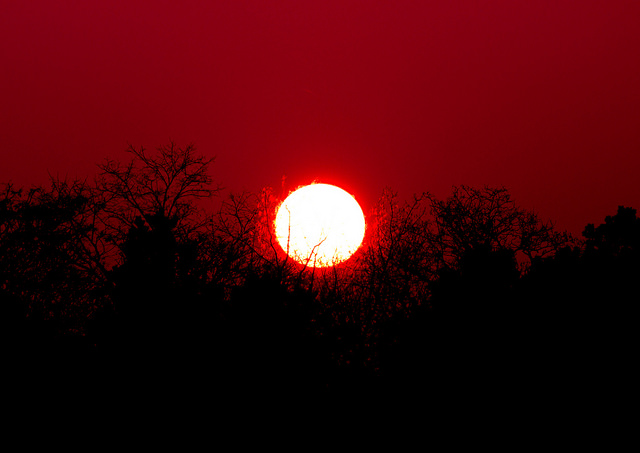
\includegraphics[width=0.5\linewidth]{images/SCP.001.when.night.breaks.jpg}
	\caption*{SCP-001激活后数分钟,拍摄者未知。}
\end{figure}

\bb{项目编号:}SCP-001

\bb{项目等级:}Apollyon

\bb{特殊收容措施:}\red{未提交更改。信息崩溃。}

\bb{描述:}\red{未提交更改。信息崩溃。}

\cl{\red{
+打开附件:事故报告-001.1\\
...\\
...\\
...\\
授予访问权限
}}

\begin{whitebox}[left=2pt, right=2pt, top=2pt, bottom=2pt]

他们一直坐在那里,呼唤并乞求我们走到外面去。噪音引来了更多人。这样庞大的一个集群,我敢肯定至少有几十个人,天晓得里面混杂了多少动物。尖叫、抱怨、怒吼和咆哮声此起彼伏,简直比地狱更响亮。最糟糕的是令人恶心的呻吟声 – 就好像他们真的在享受似的。

他们只要知道我们还在这里,就不会离去。

我们设法说服了一个D级出去看看 – 看他能不能把它们引开,他的计划令人惊讶 – 他只要了一把手枪,和一颗子弹。他走到它那儿去,随即它捉住他试图掀开他的面具,他设法将枪口抵住下巴然后扣动扳机。我想他很幸运。

他踉跄地跌倒在地,它滑进了他的防护服,撬开面罩,从内部开始将他撕裂。

他回来了;开始转化 – 曾是他身体的凝胶从衣服中滴落,尖叫尖叫尖叫。

它们甚至不让我们寻死。

主任有个计划,他的办公室里有个逃生隧道,站点下方的电车可以将我们带到一个安全屋 – 我们应该可以从那里起步,前往Site-19。

\end{whitebox}

\hr

% =====

\newpage

\tred{开启文件:SCP-001修订版\# 8/12 一(1)附件}

\tred{隐藏修订版}

\hr

\g{\bb{修订版\# 8/12更新于1200日前}}

\begin{figure}[H]
	\centering
	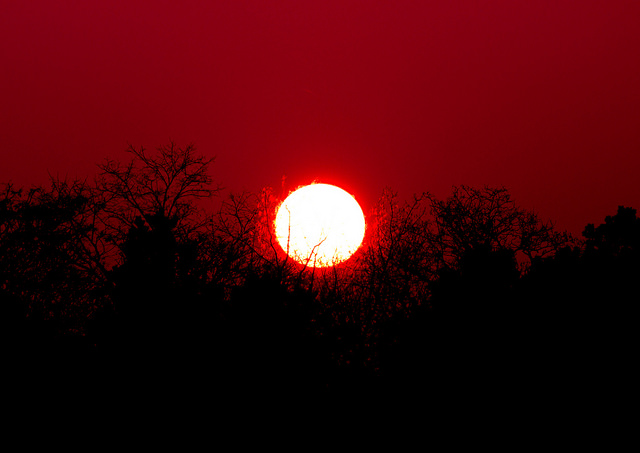
\includegraphics[width=0.5\linewidth]{images/SCP.001.when.night.breaks.jpg}
	\caption*{SCP-001激活后数分钟,拍摄者未知。}
\end{figure}

\bb{项目编号:}SCP-001

\bb{项目等级:}Apollyon

\bb{特殊收容措施:}\red{未提交更改。信息崩溃。}

\bb{描述:}\red{未提交更改。信息崩溃。}

\cl{\red{
+打开附件:音频文件\\
...\\
...\\
...\\
授予访问权限
}}

\begin{scpbox}

你第一次看到她的样貌,Igotta博士坐在你现在所处的地方,神情痛苦,双眼布满血丝,胸口处晕染着大而潮湿的黑红色。

她颤抖而短促地呼吸着,嘴唇翕动,似乎是在说话,声音却哽咽在了喉咙里。她垂下头,无声地啜泣起来,一分钟后,她设法克制住自己:

\end{scpbox}

\begin{scpdialog}

“我,我 – 我们,电 – 电车……

在隧道里,从天花板流淌下来,拖动,拖动他们进入,光 – 光剥开他们的衣服,和,和 – 和……”

\end{scpdialog}

\begin{scpbox}

她将手伸入胸前的口袋,掏出半截断指,断口下方可清晰地看到结婚戒指的暗淡光泽。她紧紧握着它,捧在手心里,拇指摸索着闪烁的金属。

她近乎永恒地呆坐着,反复低声道歉,乞求宽恕,看起来失魂落魄。片刻后她抬起头来,发现自己还在录音,好像回归了现实;她将断指塞回口袋,前倾身体,像是要关闭摄像机,但是这时一台收音机发出了声音。

它播放了几秒白噪音,而后突兀地传出了令你万分紧张的声音。

\end{scpbox}

\begin{scpdialog}
“Logan?”
\end{scpdialog}

\begin{scpbox}
那几乎是Ari的声音,然而那声音已经受到影响、如肠鸣音一般。Logan错愕地张开嘴,脸庞血色尽失。
\end{scpbox}

\begin{scpdialog}

“你在哪儿?为什么我回不到里面去?

你在吗”?

\end{scpdialog}


\begin{scpbox}
Logan从办公桌下捡起一部手持式收音机,她的手有些颤抖,那东西不断恳求着她;不成人声的嗓音让你倒尽胃口。
\end{scpbox}

\begin{scpdialog}
“宝贝,没关系,\ii{我}没事,真的。

这是个明亮而阳光灿烂的好日子,你却无所事事地虚度光阴。”
\end{scpdialog}

\begin{scpbox}
Logan泪流满面,手指盘旋在呼叫按钮上方。曾是Ari的东西用一种深沉而湿润的声调呼吸并说话。
\end{scpbox}

\begin{scpdialog}
“多么美丽而澄澈的蓝天 – 和那天一模一样,你还记得吗?”
\end{scpdialog}

\begin{scpbox}
Logan用她空闲的手拿起一支烟,而后划着火柴。她哆嗦着手指两次尝试点燃烟头却失败了。她在心底默默宣誓,第三次点燃香烟,吸了四分之一。曾是Ari的东西继续说:
\end{scpbox}

\begin{scpdialog}
“这太完美了,和我一直梦想着的一模一样,你的计划真是精巧,我从未像此刻这样感受到爱。”
\end{scpdialog}

\begin{scpbox}
Logan开始摇晃。
\end{scpbox}

\begin{scpdialog}
“甚至有乐队演奏我们的歌谣……”
\end{scpdialog}

\begin{scpbox}
它开始歌唱。
\end{scpbox}

\begin{scpdialog}
\ii{“我感觉很好,以这特殊的方式}

\ii{我坠入爱河,这是个阳光明媚的好日子”}
\end{scpdialog}

\begin{scpdialog}
Logan将收音机丢出房间,它在某处磕碎了屏幕,但仍在运作 – 你仍能听到那东西的歌声。
\end{scpdialog}

\begin{scpdialog}
\ii{“好日子,阳光明媚的好日子}\\
\ii{好日子,阳光明媚的好日子”}
\end{scpdialog}

\begin{scpbox}
随着无线电慢慢消逝,越来越多的声音齐声合唱,几个,几十个,乃至更多,他们放声歌唱,直到收音机仁慈地沉寂下去,Logan从她的椅子上跳起来冲了出去,你可以听到她在屏幕外呕吐。视频画面定格在空座位上,过了几分钟,她返回并关掉了摄影机。
\end{scpbox}

\hr

% =====

\newpage

\tred{等等,哪里不对。}

\tred{…}

\begin{scpbox}

有种挥之不去的、却又似妄想的感觉包裹着你,你正被监视。你戒备地睁大眼睛,尽管视线从显示器处移开后需片刻来适应黑暗,应急灯光扫过房间,将阴影拉伸扭曲地面目全非。这时,你发现了它。

在那儿,在那角落中。

它正从泥潭中爬出。

时间在这一刻放缓,一双手,涂满了遍布整个设施的黑色粘液,撑在了令人作呕的泥潭两侧,仿佛地板下方的东西正努力支撑,试图将自己的身体抬升起来。

不成人形。

头部随之而来,从粪便中上升,乱蓬蓬的毛发遮盖了它的脸,不明液体肆意横流,它转向你的方向。

它在角落中注视着你,而后再次沉入黑暗。

应急灯光再次穿过房间,扫射着泥潭,它看起来和方才别无二致。

\end{scpbox}

% =====

\newpage

\tred{开启文件:SCP-001修订版\#9/12 一(1)附件:}

\tred{隐藏修订版}

\hr

\g{\bb{修订版\# 9/12更新于986日前}}

\begin{figure}[H]
	\centering
	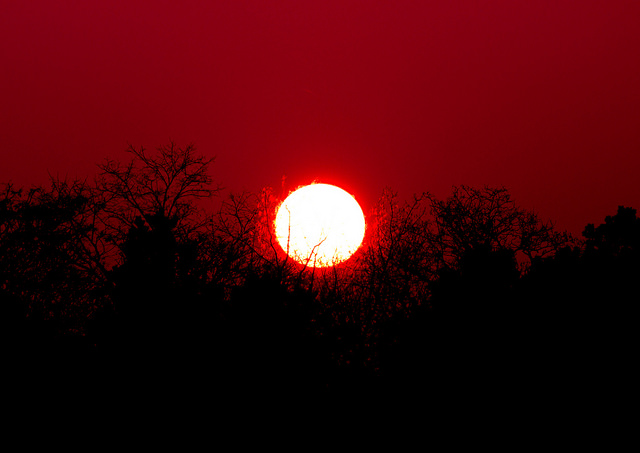
\includegraphics[width=0.5\linewidth]{images/SCP.001.when.night.breaks.jpg}
	\caption*{SCP-001激活后数分钟,拍摄者未知。}
\end{figure}

\bb{项目编号:}SCP-001

\bb{项目等级:}Apollyon

\bb{特殊收容措施:}

\bb{描述:}\red{未提交更改。信息崩溃。}

\cl{\red{
+打开附件\\
...\\
...\\
...\\
授予访问权限
}}

\begin{scpbox}
Igotta博士的身影出现在显示器上,她看起来消瘦了,大张的双眼遍布血丝。桌面上搁着一把刀,一只碗,一页表面泛黄的马尼拉信封。

上面叠着一卷染血的羊皮纸。
\end{scpbox}

\begin{scpdialog}
“虽然我们身处基金会,并且面临了这些事情,但我一直认为我们能够保持控制与收容,我们将隐匿于黑暗之中 - 令人类在光明的大道上蓬勃发展。

Site-19的通讯上月起中断了,我越来越难以找到理由坚持下去 – 尤其是,在失去了……”
\end{scpdialog}

\begin{scpbox}
她抓起刀,犹豫了片刻。
\end{scpbox}

\begin{scpdialog}
“那些声音一次又一次地在我脑海中盘旋飘荡,我时常回忆起隧道中的那天,一切事情都发生了。我已经回去过几次了,只是为了能再次听到她的声音。

但这是错误的,门那边的东西 – 不是她,她再也不会回来了。那声音听起来很像她,它也知道她所知道的一切,但它不再是她了。这光 – 它夺走你的身体,偷窃你的思想。

但你的灵魂呢?”
\end{scpdialog}

\begin{scpbox}
说到这儿,她将刀片压入左手掌心,因疼痛而抽搐。你看着她握紧拳头,令血液流入碗底
\end{scpbox}

\begin{scpdialog}
“如果这样做……能让我寻回失去的,光线无法企及之物;我会回来更新的。现在我说完了。”
\end{scpdialog}

\hr

% =====

\newpage

\tred{开启文件:SCP-001修订版\# 17!24ATA错误}

\tred{隐瞒我}

\hr

\g{\bb{修订版4847/3RR0R更新于985日前}}

\begin{figure}[H]
	\centering
	
\includegraphics[width=0.5\linewidth]{images/SCP.001.when.night.breaks.2.jpg}
	\caption*{它是多么温暖。}
\end{figure}

\bb{编号。}伤害。

\bb{项目。}Apologize

\bb{特殊收容措施:}SCP-001\bb{不应}被收容,SCP-001事件幸存者将驻扎在安全设施中并永远无法彼此保持联系,鼓励人员\bb{克服自身,停止思考他们所知之事。}

\bb{你不可能永远隐匿此处,吾爱。}

暴露于SCP-001的人员将\bb{不可}被遗弃,我没有要求你救我,这不是你所做的选择。 请\textsuperscript{
不要不要不要不要不要不要不要}尝试安乐死。

已证实电导武器\bb{为什么?}在固定情况下有一定作用。\bb{你无法忍受我变得更好。}燃烧器\bb{如同瘙痒。}迄今为止,冷冻弹药是最有效的。

驻扎在Site-19的人员将\bb{不遗余力,我也是,永远不会太晚,宝贝。}

\bb{描述:}SCP-001是\bb{我们终获自由后}对于太阳的称谓,其影响是瞬时的,\bb{将将你从所有痛苦中解放, 直至你将我撕裂。这种变化看起来很吓人,我明白,}尽管经历了这种充足,但你\bb{不会死。}

\bb{我保证。}

由于它们的物质组成,SCP-001-A个体可通过彼此接触进行分子水平上的联接和混合\bb{并最终以这种形态存在}。这不会造成\bb{任何痛苦}。自SCP-001-A事件以来,大多数个体已集聚为这样的集群,似乎不存在最大融合上限。\textcolor{white}{不要担忧}

所得的生物质是\textsuperscript{美}\bb{丽}\textsubscript{的},集群中的生物体将在其内部和周围游移,\textsubscript{进入}\textsuperscript{分离}\textsubscript{进入}\textsuperscript{分离}\textsubscript{进入} - 其中肢体和身体部分都将转移\bb{永不放弃}。 \textsubscript{万物归一}随后恶化并被另一种生命形态纳入。

集群中的个体仅是想要再度靠近你。

如此努力。\\
\small{让我进入}

\g{\bb{带我回去}}

\begin{scpbox}

附有一个视频文件,打开它,你将看到它拍摄者你所身处的房间,画面似乎来自一个设置在房间角落的监控摄像头。环境十分昏暗,但你可辨认出Igotta博士,躺在远处墙边堆放的衣物上。

她在睡眠中不安地扭动身体,似乎正承受着折磨和伤害。她辗转反侧,嘟囔着无意义的音节。

摄像头抖动,微微向上抬起,而后再次重点关注她。

它开始缓慢靠近。

扬声器开启;你听到了轻而平缓的呼吸,随着摄像头靠近博士,这声音愈发清晰,逼真。不仅仅是白噪声,而是又几十个 – 几百个声音共同组成的含糊不清的耳语。

你靠了过去,几乎将耳朵贴在了扬声器上,试图弄明白它们在说什么。由不一致声中脱颖而出的却是:

\end{scpbox}

\cl{
你在注意?\\
下一幕便是为你而设。
}

\begin{scpbox}

不过你不太确定该怎么做,回顾显示器,镜头已停顿在距睡着的博士差不多一英寸之处,

噪声停止了。

悄无声息。

一只手,黑而油腻,且瘦骨嶙峋,伸向她的前额,撩开了一缕头发。

她猛地睁开眼睛,震惊地反击,视频切断了。

\end{scpbox}

\hr

% =====

\newpage

\tred{开启文件:SCP-001修订版\# 9/12一(1)附件:}

\tred{隐藏修订版}

\hr

\g{\bb{修订版\# 12/12更新于1日前}}

\begin{figure}[H]
	\centering
	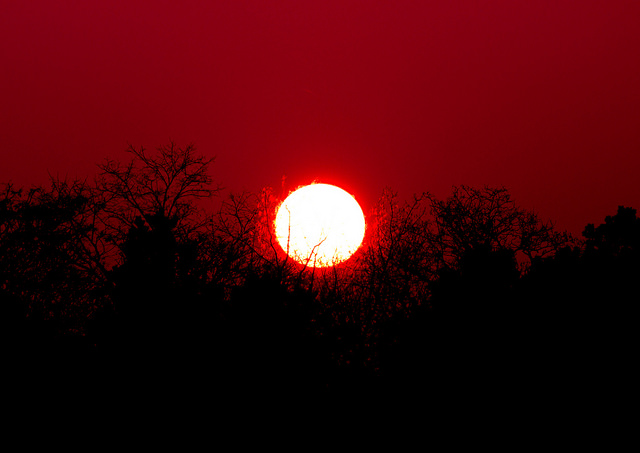
\includegraphics[width=0.5\linewidth]{images/SCP.001.when.night.breaks.jpg}
	\caption*{SCP-001激活后数分钟,拍摄者未知。}
\end{figure}

\bb{项目编号:}SCP-001

\bb{项目等级:}Apollyon

\bb{特殊收容措施:}\red{文件恢复于此前版本。信息崩溃。}

\bb{描述:}\red{文件恢复于此前版本。信息崩溃。}

\cl{\red{
+打开附件\\
...\\
...\\
...\\
授予访问权限
}}

\begin{scpbox}
Igotta博士出现在画面中,状态看起来比以前更加糟糕,头发明显稀疏,中间缺了大片。若不是正反射着显示器的柔和光芒,你甚至会以为她不再拥有双眼,因为它们已深陷入了她的眼窝之中。她眼睛一眨不眨地凝视着前方。
\end{scpbox}

\begin{scpdialog}
“她不会停止,她,她从未离去,我知道我没有,没有因浏览文档感染信息危害。我测试自己是否受到-4673感染,答案是否定的。-5189是,是唯一,唯一使用打印作为载体的,不 – 不是,我仍拥有全部的手指!”
\end{scpdialog}

\begin{scpbox}
她咧开双唇,露出一个破碎的笑容,她微弱地笑着,露出颤抖的双手,似乎曾是手指的骨骼遗骸大部分嵌入了她左手的血肉之中 – 支撑着她无名指处的残肢。两枚婚戒松散地套在上面,彼此相碰。
\end{scpbox}

\begin{scpdialog}
“所以,我没有感染,我不是,没有,我,我没有发疯。我知道,我知道仪式如何运转,我知道这真的是她,是她的,她——”
\end{scpdialog}

\begin{scpbox}
有些东西使她的注意力离开屏幕,她转首听着。
\end{scpbox}

\begin{scpdialog}
“不!不,我不 – 不能!你不是,不是你,这不一样。不是你,这再也不是你了,不!不不不!
\end{scpdialog}

\begin{scpbox}
她用力揉着自己的太阳穴,一遍又一遍地重复道。一分钟后,她转回头,面对摄像机。
\end{scpbox}

\begin{scpdialog}
“它是她又不是,我所带回的 – 仍然是一部分,没办法,束手无策,无可挽回。

未来对我来说毫无希望,上帝啊,我不能再这样下去了。

我在这儿很安全,光线无法到我身边 – 我,我不 – 不会让它,让它带走我。
\end{scpdialog}

\begin{scpbox}
她挥舞着一把手枪。
\end{scpbox}

\begin{scpdialog}
我本来计 – 计划用这个,直到我找到了剩下的,剩下的药物。我不想冒险,冒险将它们的注意力转移到我 - 我的身上……我的身体。
\end{scpdialog}

\begin{scpbox}
她拉开办公桌的抽屉,放好手枪,抬起眼皮凝视着摄像头。
\end{scpbox}

\begin{scpdialog}
妈妈,爸爸,Ari。

我很抱歉。”
\end{scpdialog}

\begin{scpbox}
她前倾身体,记录结束。
\end{scpbox}

\hr

% =====

\newpage

\tred{太可怕了}

\tred{就这样结束了吗?}

\begin{scpbox}
你拉开抽屉,抽出手枪,心不在焉地在手里翻弄了一会儿,想知道你该到那里去。Site-17?64?当然你不会是最后的幸存者。电脑发出声响,文件有更新吗?
\end{scpbox}

% =====

\newpage

\tred{访问SCP-001:当前迭代更新于一(1)分钟前}

\tred{__}

\hr

\bb{项目编号:}

\cl{
\ii{炽日升上了藏红花似的天空\\
偶然地相逢,彼此不安地表现\\
终有一日,吾爱,我们二者将}
}

\bb{项目等级:}

\cl{
\ii{融为一体,进程就此开始\\
浓雾迷乱而狂野,闪耀光辉;\\
旭日的光芒四射于湛蓝的晴空}
}

\bb{特殊收容措施:}

\cl{
\ii{就在我们奋力奔跑之时\\
穿越隧道,狂野的热潮,\\
那日,吾爱,我们终将拥有}

\ii{共度的未来 – 我们所赢得的生活\\
承诺与责任,为我们组建的家庭\\
蔚蓝的天空埋葬了闪耀的}
}

\bb{描述:}

\cl{
\ii{阳光,被命运淹没 – 超支\\
愤怒与怨恨肆意滋生\\
昨日,吾爱,你我尚为一体}

\ii{此刻你静卧于此,你的生命已离去\\
徘徊于她射线外的黑暗\\
绯红的天幕在火炬下烧灼;我们的太阳,\\
今日,吾爱,我们融为一体}
}

\begin{figure}[H]
	\centering
	
\includegraphics[width=0.5\linewidth]{images/SCP.001.when.night.breaks.3.jpg}
	\caption*{系统错误误误误误误误误误\# @\& \# .}
\end{figure}

\hr

% =====

\newpage

\begin{scpbox}

没有你的命令,显示器开始自动播放视频文件,当你看到加载出的图像时,寒意涌上心头。

这是一幕实时录像,来自你的背后,距离大约一英尺远。

一只骨瘦如柴的墨色左手进入画面,极缓慢地接近你。它没有无名指。

再来不及思考更多,你疯狂的转过身来举枪射击,希望能驱散幽灵。

你的子弹射入一面空荡荡的墙壁,此处一无所有。

在你听到它之前,有什么东西再度经过 – 在你听到它们的声音之前。流淌着的湿润的抨击伴随着尖声合唱涌入走廊。

它撞击着屋门,此处莫不是藏身之所?

它再度撞击,似乎有一张脸浮现出来,某一部分属于人类,其余部分则……是某些东西 - 正从缝隙中缓慢灌入。血肉从神知道由何而来的淤泥中渗出,重新组合成手指、眼睛与羽毛。

第三次。它此刻正压在木梁上,沉甸甸地使之向内下垂。

伴随着呻吟与破裂声,木梁支离破碎,门打开了。

手掌和臂膊拉起你,一个接一个地将你传递出去,经由空的收容单元,继续向上,穿过楼梯间,通往大厅和隧道。

你所拥有的宝贵黑暗不过片刻。

隧道的尽头,有光。

\end{scpbox}

